\documentclass[a4paper]{book}
\usepackage{a4wide}
\usepackage{makeidx}
\usepackage{fancyhdr}
\usepackage{graphicx}
\usepackage{multicol}
\usepackage{float}
\usepackage{textcomp}
\usepackage{alltt}
\usepackage{doxygen}
\makeindex
\setcounter{tocdepth}{1}
\renewcommand{\footrulewidth}{0.4pt}
\begin{document}
\begin{titlepage}
\vspace*{7cm}
\begin{center}
{\Large AZURE Reference Manual\\[1ex]\large 2.0 }\\
\vspace*{1cm}
{\large Generated by Doxygen 1.4.7}\\
\vspace*{0.5cm}
{\small Fri May 28 15:47:44 2010}\\
\end{center}
\end{titlepage}
\clearemptydoublepage
\pagenumbering{roman}
\tableofcontents
\clearemptydoublepage
\pagenumbering{arabic}
\chapter{AZURE R-Matrix Package }
\label{index}AZURE is created to be general A-/R- Matrix program for the analysis of data relavent to nuclear astrophysics. This release of AZURE has been completely rewritten in object-oriented C++. The documentation contained within these pages should serve as an introduction to the object structure of AZURE Version 2.0. 
\chapter{AZURE Hierarchical Index}
\section{AZURE Class Hierarchy}
This inheritance list is sorted roughly, but not completely, alphabetically:\begin{CompactList}
\item \contentsline{section}{AChannel}{\pageref{classAChannel}}{}
\item \contentsline{section}{ALevel}{\pageref{classALevel}}{}
\item \contentsline{section}{AZURECalc}{\pageref{classAZURECalc}}{}
\item \contentsline{section}{AZUREFBuffer}{\pageref{classAZUREFBuffer}}{}
\item \contentsline{section}{AZUREMain}{\pageref{classAZUREMain}}{}
\item \contentsline{section}{AZUREOutput}{\pageref{classAZUREOutput}}{}
\item \contentsline{section}{CNuc}{\pageref{classCNuc}}{}
\item \contentsline{section}{Config}{\pageref{structConfig}}{}
\item \contentsline{section}{Coul\-Func}{\pageref{classCoulFunc}}{}
\item \contentsline{section}{Coul\-Waves}{\pageref{structCoulWaves}}{}
\item \contentsline{section}{Decay}{\pageref{classDecay}}{}
\item \contentsline{section}{ECIntegral}{\pageref{classECIntegral}}{}
\item \contentsline{section}{ECInt\-Result}{\pageref{structECIntResult}}{}
\item \contentsline{section}{ECLevel}{\pageref{classECLevel}}{}
\item \contentsline{section}{ECMGroup}{\pageref{classECMGroup}}{}
\item \contentsline{section}{EData}{\pageref{classEData}}{}
\item \contentsline{section}{Energy\-Map}{\pageref{structEnergyMap}}{}
\item \contentsline{section}{EPoint}{\pageref{classEPoint}}{}
\item \contentsline{section}{ESegment}{\pageref{classESegment}}{}
\item \contentsline{section}{Gen\-Matrix\-Func}{\pageref{classGenMatrixFunc}}{}
\begin{CompactList}
\item \contentsline{section}{AMatrix\-Func}{\pageref{classAMatrixFunc}}{}
\item \contentsline{section}{RMatrix\-Func}{\pageref{classRMatrixFunc}}{}
\end{CompactList}
\item \contentsline{section}{Interference}{\pageref{classInterference}}{}
\item \contentsline{section}{JGroup}{\pageref{classJGroup}}{}
\item \contentsline{section}{KGroup}{\pageref{classKGroup}}{}
\item \contentsline{section}{KLGroup}{\pageref{classKLGroup}}{}
\item \contentsline{section}{MGroup}{\pageref{classMGroup}}{}
\item \contentsline{section}{NFIntegral}{\pageref{classNFIntegral}}{}
\item \contentsline{section}{PPair}{\pageref{classPPair}}{}
\item \contentsline{section}{Reaction\-Rate}{\pageref{classReactionRate}}{}
\item \contentsline{section}{Shft\-Func}{\pageref{classShftFunc}}{}
\item \contentsline{section}{Temp\-TMatrix}{\pageref{structTempTMatrix}}{}
\item \contentsline{section}{Whit\-Func}{\pageref{classWhitFunc}}{}
\end{CompactList}

\chapter{AZURE Class Index}
\section{AZURE Class List}
Here are the classes, structs, unions and interfaces with brief descriptions:\begin{CompactList}
\item\contentsline{section}{\bf{AChannel} (An AZURE channel object )}{\pageref{classAChannel}}{}
\item\contentsline{section}{\bf{ALevel} (An AZURE level object )}{\pageref{classALevel}}{}
\item\contentsline{section}{\bf{AMatrix\-Func} (A function class to calculate the T-Matrix using the A-Matrix )}{\pageref{classAMatrixFunc}}{}
\item\contentsline{section}{\bf{AZURECalc} (A function class to perform the calculation of the chi-squared value )}{\pageref{classAZURECalc}}{}
\item\contentsline{section}{\bf{AZUREFBuffer} (A container class for a pointer to a file buffer )}{\pageref{classAZUREFBuffer}}{}
\item\contentsline{section}{\bf{AZUREMain} (The top-level AZURE function class )}{\pageref{classAZUREMain}}{}
\item\contentsline{section}{\bf{AZUREOutput} (A class to assist in writing AZURE output files )}{\pageref{classAZUREOutput}}{}
\item\contentsline{section}{\bf{CNuc} (An AZURE compound nucleus )}{\pageref{classCNuc}}{}
\item\contentsline{section}{\bf{Config} (A configuration structure for AZURE )}{\pageref{structConfig}}{}
\item\contentsline{section}{\bf{Coul\-Func} (A function class to calculate Coulomb functions for positive energy channels )}{\pageref{classCoulFunc}}{}
\item\contentsline{section}{\bf{Coul\-Waves} (The return structure of the \doxyref{Coul\-Func}{p.}{classCoulFunc} function class )}{\pageref{structCoulWaves}}{}
\item\contentsline{section}{\bf{Decay} (An AZURE decay pair )}{\pageref{classDecay}}{}
\item\contentsline{section}{\bf{ECIntegral} (A function class to calculate external capture integrals )}{\pageref{classECIntegral}}{}
\item\contentsline{section}{\bf{ECInt\-Result} (Return structure for \doxyref{ECIntegral}{p.}{classECIntegral} function class )}{\pageref{structECIntResult}}{}
\item\contentsline{section}{\bf{ECLevel} (An AZURE external capture component )}{\pageref{classECLevel}}{}
\item\contentsline{section}{\bf{ECMGroup} (An AZURE external reaction pathway )}{\pageref{classECMGroup}}{}
\item\contentsline{section}{\bf{EData} (An AZURE data object )}{\pageref{classEData}}{}
\item\contentsline{section}{\bf{Energy\-Map} (A container structure for a reference to a data point )}{\pageref{structEnergyMap}}{}
\item\contentsline{section}{\bf{EPoint} (An AZURE data point )}{\pageref{classEPoint}}{}
\item\contentsline{section}{\bf{ESegment} (An AZURE data segment )}{\pageref{classESegment}}{}
\item\contentsline{section}{\bf{Gen\-Matrix\-Func} (A generalized function class to calculate cross sections )}{\pageref{classGenMatrixFunc}}{}
\item\contentsline{section}{\bf{Interference} (An AZURE $ l_1,l_2,l_1',l_2',J_1,J_2 $ combination )}{\pageref{classInterference}}{}
\item\contentsline{section}{\bf{JGroup} (An AZURE $ J^\pi $ group )}{\pageref{classJGroup}}{}
\item\contentsline{section}{\bf{KGroup} (An AZURE $ s,s' $ group )}{\pageref{classKGroup}}{}
\item\contentsline{section}{\bf{KLGroup} (An AZURE $ s,s',L $ group )}{\pageref{classKLGroup}}{}
\item\contentsline{section}{\bf{MGroup} (An AZURE internal reaction pathway )}{\pageref{classMGroup}}{}
\item\contentsline{section}{\bf{NFIntegral} (A function class to calculate the channel integrals in the denominator of the $ N_f^{1/2} $ term )}{\pageref{classNFIntegral}}{}
\item\contentsline{section}{\bf{PPair} (An AZURE Particle Pair )}{\pageref{classPPair}}{}
\item\contentsline{section}{\bf{Reaction\-Rate} (A function class to calculate the reaction rate )}{\pageref{classReactionRate}}{}
\item\contentsline{section}{\bf{RMatrix\-Func} (A function class to calculate the T-Matrix using the R-Matrix )}{\pageref{classRMatrixFunc}}{}
\item\contentsline{section}{\bf{Shft\-Func} (A function class for negative energy shift functions )}{\pageref{classShftFunc}}{}
\item\contentsline{section}{\bf{Temp\-TMatrix} (A temporaray T-Matrix structure )}{\pageref{structTempTMatrix}}{}
\item\contentsline{section}{\bf{Whit\-Func} (A function class to calculate Whittaker functions for negative energy channels )}{\pageref{classWhitFunc}}{}
\end{CompactList}

\chapter{AZURE Class Documentation}
\section{AChannel Class Reference}
\label{classAChannel}\index{AChannel@{AChannel}}
An AZURE channel object.  


{\tt \#include $<$AChannel.h$>$}

\subsection*{Public Member Functions}
\begin{CompactItemize}
\item 
\bf{AChannel} (Nuc\-Line, int)
\item 
\bf{AChannel} (int, double, int, char)
\item 
int \bf{Get\-Pair\-Num} () const 
\item 
int \bf{Get\-L} () const 
\item 
double \bf{Get\-S} () const 
\item 
double \bf{Get\-Boundary\-Condition} () const 
\item 
char \bf{Get\-Rad\-Type} () const 
\item 
void \bf{Set\-Boundary\-Condition} (double)
\end{CompactItemize}


\subsection{Detailed Description}
An AZURE channel object. 

An R-Matrix channel for a given $J^\pi$ group represents a specfic combination of $ \alpha,s,l $ couplings. 



\subsection{Constructor \& Destructor Documentation}
\index{AChannel@{AChannel}!AChannel@{AChannel}}
\index{AChannel@{AChannel}!AChannel@{AChannel}}
\subsubsection{\setlength{\rightskip}{0pt plus 5cm}AChannel::AChannel (Nuc\-Line {\em nuc\-Line}, int {\em pair\-Num})}\label{classAChannel_556c9f764e458ae0a592339b2ccd3ac9}


This constructor can be used if a channel is to be created from a specific line of the nuclear input file. \index{AChannel@{AChannel}!AChannel@{AChannel}}
\index{AChannel@{AChannel}!AChannel@{AChannel}}
\subsubsection{\setlength{\rightskip}{0pt plus 5cm}AChannel::AChannel (int {\em l\-Value}, double {\em s\-Value}, int {\em pair\-Num}, char {\em rad\-Type})}\label{classAChannel_62160323fe4a68af2b7a7c5ec941be8a}


This constructor can be used if a channel is to be created directly using specified channel couplings. 

\subsection{Member Function Documentation}
\index{AChannel@{AChannel}!GetBoundaryCondition@{GetBoundaryCondition}}
\index{GetBoundaryCondition@{GetBoundaryCondition}!AChannel@{AChannel}}
\subsubsection{\setlength{\rightskip}{0pt plus 5cm}double AChannel::Get\-Boundary\-Condition () const}\label{classAChannel_aaa76e0abc5d42245e4492101d300533}


Returns the boundary condition for the channel. The energy of the boundary condition is fixed at the first level given in the nuclear input file for a given $ J^\pi $ group. \index{AChannel@{AChannel}!GetL@{GetL}}
\index{GetL@{GetL}!AChannel@{AChannel}}
\subsubsection{\setlength{\rightskip}{0pt plus 5cm}int AChannel::Get\-L () const}\label{classAChannel_6034d5c938ccc6f87376f7a27df05fd8}


Returns the orbital angular momentum for the channel. \index{AChannel@{AChannel}!GetPairNum@{GetPairNum}}
\index{GetPairNum@{GetPairNum}!AChannel@{AChannel}}
\subsubsection{\setlength{\rightskip}{0pt plus 5cm}int AChannel::Get\-Pair\-Num () const}\label{classAChannel_b171ddbcd632358ebbcfb294e5f39549}


Returns the pair number, or position of the corresponding particle pair in the \doxyref{PPair}{p.}{classPPair} vector, for the channel. \index{AChannel@{AChannel}!GetRadType@{GetRadType}}
\index{GetRadType@{GetRadType}!AChannel@{AChannel}}
\subsubsection{\setlength{\rightskip}{0pt plus 5cm}char AChannel::Get\-Rad\-Type () const}\label{classAChannel_f0b07c80e95c906eb79f945c934289d8}


Returns the radiation type for the channel. Radiation types are:\begin{itemize}
\item P: Particle Radiation\item E: EL Electromagnetic Radiation\item M: ML Electromagnetic Radiation \end{itemize}
\index{AChannel@{AChannel}!GetS@{GetS}}
\index{GetS@{GetS}!AChannel@{AChannel}}
\subsubsection{\setlength{\rightskip}{0pt plus 5cm}double AChannel::Get\-S () const}\label{classAChannel_ea5b7de816a89315731b7fa50262f7f4}


Returns the coupled channel spin for the channel. \index{AChannel@{AChannel}!SetBoundaryCondition@{SetBoundaryCondition}}
\index{SetBoundaryCondition@{SetBoundaryCondition}!AChannel@{AChannel}}
\subsubsection{\setlength{\rightskip}{0pt plus 5cm}void AChannel::Set\-Boundary\-Condition (double {\em boundary\-Condition})}\label{classAChannel_c97e3a820c80ea0ef74723cc89ca7fdf}


This function is used to set the boundary condition for the channel. 

The documentation for this class was generated from the following files:\begin{CompactItemize}
\item 
azure\_\-v2/include/AChannel.h\item 
azure\_\-v2/src/AChannel.cpp\end{CompactItemize}

\section{ALevel Class Reference}
\label{classALevel}\index{ALevel@{ALevel}}
An AZURE level object.  


{\tt \#include $<$ALevel.h$>$}

\subsection*{Public Member Functions}
\begin{CompactItemize}
\item 
\bf{ALevel} (Nuc\-Line)
\item 
\bf{ALevel} (double)
\item 
bool \bf{Is\-In\-RMatrix} () const 
\item 
bool \bf{Energy\-Fixed} () const 
\item 
bool \bf{Channel\-Fixed} (int) const 
\item 
int \bf{Num\-NFIntegrals} () const 
\item 
int \bf{Get\-Transform\-Iterations} () const 
\item 
double \bf{Get\-E} () const 
\item 
double \bf{Get\-Gamma} (int) const 
\item 
double \bf{Get\-Fit\-Gamma} (int) const 
\item 
double \bf{Get\-Fit\-E} () const 
\item 
double \bf{Get\-NFIntegral} (int) const 
\item 
double \bf{Get\-Sqrt\-NFFactor} () const 
\item 
double \bf{Get\-ECConversion\-Factor} (int) const 
\item 
double \bf{Get\-Transform\-Gamma} (int) const 
\item 
double \bf{Get\-Transform\-E} () const 
\item 
double \bf{Get\-Big\-Gamma} (int) const 
\item 
std::complex$<$ double $>$ \bf{Get\-External\-Gamma} (int) const 
\item 
void \bf{Add\-Gamma} (Nuc\-Line)
\item 
void \bf{Add\-Gamma} (double)
\item 
void \bf{Set\-Gamma} (int, double)
\item 
void \bf{Set\-E} (double)
\item 
void \bf{Set\-Fit\-Gamma} (int, double)
\item 
void \bf{Set\-Fit\-E} (double)
\item 
void \bf{Add\-NFIntegral} (double)
\item 
void \bf{Set\-Sqrt\-NFFactor} (double)
\item 
void \bf{Add\-ECConversion\-Factor} (double)
\item 
void \bf{Set\-Transform\-Gamma} (int, double)
\item 
void \bf{Set\-Transform\-E} (double)
\item 
void \bf{Set\-Big\-Gamma} (int, double)
\item 
void \bf{Set\-Transform\-Iterations} (int)
\item 
void \bf{Set\-External\-Gamma} (int, std::complex$<$ double $>$)
\end{CompactItemize}


\subsection{Detailed Description}
An AZURE level object. 

An R-matrix level represents a specific eigenstate of the compound nucleus. 



\subsection{Constructor \& Destructor Documentation}
\index{ALevel@{ALevel}!ALevel@{ALevel}}
\index{ALevel@{ALevel}!ALevel@{ALevel}}
\subsubsection{\setlength{\rightskip}{0pt plus 5cm}ALevel::ALevel (Nuc\-Line {\em nuc\-Line})}\label{classALevel_aa406d92786470eb211e9fa0f5ba5496}


This constructor is used when a level object is created from an entry in the nuclear file. \index{ALevel@{ALevel}!ALevel@{ALevel}}
\index{ALevel@{ALevel}!ALevel@{ALevel}}
\subsubsection{\setlength{\rightskip}{0pt plus 5cm}ALevel::ALevel (double {\em energy})}\label{classALevel_e9c0cda96b6300572e75beade96eb0ca}


This constructor is used when a level object is created using a specific energy. 

\subsection{Member Function Documentation}
\index{ALevel@{ALevel}!AddECConversionFactor@{AddECConversionFactor}}
\index{AddECConversionFactor@{AddECConversionFactor}!ALevel@{ALevel}}
\subsubsection{\setlength{\rightskip}{0pt plus 5cm}void ALevel::Add\-ECConversion\-Factor (double {\em conversion\-Factor})}\label{classALevel_fb03bc09889b8f81773eb05ccc11e54b}


This function adds a conversion factor from reduced width amplitude to ANC. \index{ALevel@{ALevel}!AddGamma@{AddGamma}}
\index{AddGamma@{AddGamma}!ALevel@{ALevel}}
\subsubsection{\setlength{\rightskip}{0pt plus 5cm}void ALevel::Add\-Gamma (double {\em reduced\-Width})}\label{classALevel_c7caa4d63534a97745d9b9507c46a05a}


This function adds a position in the width vectors corresponding to a new channel. The initial reduced width amplitude is set directly. \index{ALevel@{ALevel}!AddGamma@{AddGamma}}
\index{AddGamma@{AddGamma}!ALevel@{ALevel}}
\subsubsection{\setlength{\rightskip}{0pt plus 5cm}void ALevel::Add\-Gamma (Nuc\-Line {\em nuc\-Line})}\label{classALevel_972a2181abf39f8ebc035530bdf0a890}


This function adds a position in the width vectors corresponding to a new channel. The initial reduced width amplitude is set from an entry in the nuclear input file. \index{ALevel@{ALevel}!AddNFIntegral@{AddNFIntegral}}
\index{AddNFIntegral@{AddNFIntegral}!ALevel@{ALevel}}
\subsubsection{\setlength{\rightskip}{0pt plus 5cm}void ALevel::Add\-NFIntegral (double {\em integral})}\label{classALevel_18a1700f5bf7b91e240fb4c1307ffb27}


This function creates and fills a position for the channel integral in the denominator of the $N_f^{1/2}$ term. The integral is of the form $ \int_a^\infty \left[ \frac{W_c(kr)}{W_c{ka_c}} \right]^2 $. \index{ALevel@{ALevel}!ChannelFixed@{ChannelFixed}}
\index{ChannelFixed@{ChannelFixed}!ALevel@{ALevel}}
\subsubsection{\setlength{\rightskip}{0pt plus 5cm}bool ALevel::Channel\-Fixed (int {\em channel\-Num}) const}\label{classALevel_78daf0cd95cdef89c0a742fb796c70aa}


Returns true if the reduced width amplitude for corresponding channel number is to be fixed in the fitting process, otherwise returns false. \index{ALevel@{ALevel}!EnergyFixed@{EnergyFixed}}
\index{EnergyFixed@{EnergyFixed}!ALevel@{ALevel}}
\subsubsection{\setlength{\rightskip}{0pt plus 5cm}bool ALevel::Energy\-Fixed () const}\label{classALevel_ab127808b9f980219acb20963b8ed0b3}


Returns true if the level energy is to be fixed in the fitting process, otherwise returns false. \index{ALevel@{ALevel}!GetBigGamma@{GetBigGamma}}
\index{GetBigGamma@{GetBigGamma}!ALevel@{ALevel}}
\subsubsection{\setlength{\rightskip}{0pt plus 5cm}double ALevel::Get\-Big\-Gamma (int {\em channel\-Num}) const}\label{classALevel_2f21c67d6773bc665e4203d53013631a}


Returns the Breit-Wigner partial width for a given channel number. \index{ALevel@{ALevel}!GetE@{GetE}}
\index{GetE@{GetE}!ALevel@{ALevel}}
\subsubsection{\setlength{\rightskip}{0pt plus 5cm}double ALevel::Get\-E () const}\label{classALevel_aa22d7e25798d04d69bab208d3c4e7e4}


Returns the energy of the level. \index{ALevel@{ALevel}!GetECConversionFactor@{GetECConversionFactor}}
\index{GetECConversionFactor@{GetECConversionFactor}!ALevel@{ALevel}}
\subsubsection{\setlength{\rightskip}{0pt plus 5cm}double ALevel::Get\-ECConversion\-Factor (int {\em channel\-Num}) const}\label{classALevel_4d41dd96f513eb5c7232da5077d50995}


Returns the conversion factor from reduced width amplitude to ANC for a given channel number. \index{ALevel@{ALevel}!GetExternalGamma@{GetExternalGamma}}
\index{GetExternalGamma@{GetExternalGamma}!ALevel@{ALevel}}
\subsubsection{\setlength{\rightskip}{0pt plus 5cm}std::complex$<$ double $>$ ALevel::Get\-External\-Gamma (int {\em channel\-Num}) const}\label{classALevel_4f3b10f52fcfc9f4f3c8abcb2a396a60}


Returns the external portion of the reduced width amplitude for a given channel number. \index{ALevel@{ALevel}!GetFitE@{GetFitE}}
\index{GetFitE@{GetFitE}!ALevel@{ALevel}}
\subsubsection{\setlength{\rightskip}{0pt plus 5cm}double ALevel::Get\-Fit\-E () const}\label{classALevel_c44f25d7d8117ae4602edaca92a8e2c8}


Returns the fitted energy of the level. \index{ALevel@{ALevel}!GetFitGamma@{GetFitGamma}}
\index{GetFitGamma@{GetFitGamma}!ALevel@{ALevel}}
\subsubsection{\setlength{\rightskip}{0pt plus 5cm}double ALevel::Get\-Fit\-Gamma (int {\em channel\-Num}) const}\label{classALevel_40c97f2b98a5462463d99eab30bc0759}


Returns the fitted internal reduced width amplitude for a given channel number. \index{ALevel@{ALevel}!GetGamma@{GetGamma}}
\index{GetGamma@{GetGamma}!ALevel@{ALevel}}
\subsubsection{\setlength{\rightskip}{0pt plus 5cm}double ALevel::Get\-Gamma (int {\em channel\-Num}) const}\label{classALevel_d9a5bfa377381e871e873a0bf98ad34a}


Returns the internal reduced width amplitude for a given channel number. \index{ALevel@{ALevel}!GetNFIntegral@{GetNFIntegral}}
\index{GetNFIntegral@{GetNFIntegral}!ALevel@{ALevel}}
\subsubsection{\setlength{\rightskip}{0pt plus 5cm}double ALevel::Get\-NFIntegral (int {\em channel\-Num}) const}\label{classALevel_bf0c916fcfffe3bd2c6579e62f5187d8}


Returns the calculated channel integral in the denominator of the $N_f^{1/2} $ term for a given channel number. \index{ALevel@{ALevel}!GetSqrtNFFactor@{GetSqrtNFFactor}}
\index{GetSqrtNFFactor@{GetSqrtNFFactor}!ALevel@{ALevel}}
\subsubsection{\setlength{\rightskip}{0pt plus 5cm}double ALevel::Get\-Sqrt\-NFFactor () const}\label{classALevel_d30896b8e21011a2ebca8d2e2e634ca1}


Returns the $N_f^{1/2}$ term for the level. \index{ALevel@{ALevel}!GetTransformE@{GetTransformE}}
\index{GetTransformE@{GetTransformE}!ALevel@{ALevel}}
\subsubsection{\setlength{\rightskip}{0pt plus 5cm}double ALevel::Get\-Transform\-E () const}\label{classALevel_9a0e4a0e05a1db6898ed7cb0233fe969}


Returns the physical level energy. \index{ALevel@{ALevel}!GetTransformGamma@{GetTransformGamma}}
\index{GetTransformGamma@{GetTransformGamma}!ALevel@{ALevel}}
\subsubsection{\setlength{\rightskip}{0pt plus 5cm}double ALevel::Get\-Transform\-Gamma (int {\em channel\-Num}) const}\label{classALevel_9db61f904cf1dee62de0e84d211d07ca}


Returns the physical internal reduced width amplitude for a given channel number. \index{ALevel@{ALevel}!GetTransformIterations@{GetTransformIterations}}
\index{GetTransformIterations@{GetTransformIterations}!ALevel@{ALevel}}
\subsubsection{\setlength{\rightskip}{0pt plus 5cm}int ALevel::Get\-Transform\-Iterations () const}\label{classALevel_61023b8c28d5b6d219ca6a1240b7f7d7}


Returns the number of iterations required to transform the level from formal to physical parameters. \index{ALevel@{ALevel}!IsInRMatrix@{IsInRMatrix}}
\index{IsInRMatrix@{IsInRMatrix}!ALevel@{ALevel}}
\subsubsection{\setlength{\rightskip}{0pt plus 5cm}bool ALevel::Is\-In\-RMatrix () const}\label{classALevel_676875f3240be1331290b09b6d0b207a}


Returns true if the level is to be included in the A-/R-Matrix calculation, otherwise returns false. A level may specify a bound state for external capture, but may not be an R-Matrix state (i.e. subthreshold state). \index{ALevel@{ALevel}!NumNFIntegrals@{NumNFIntegrals}}
\index{NumNFIntegrals@{NumNFIntegrals}!ALevel@{ALevel}}
\subsubsection{\setlength{\rightskip}{0pt plus 5cm}int ALevel::Num\-NFIntegrals () const}\label{classALevel_e1bf8431aea6b6037271219d118e3808}


Returns non-zero only if the level is a final state for external capture. \index{ALevel@{ALevel}!SetBigGamma@{SetBigGamma}}
\index{SetBigGamma@{SetBigGamma}!ALevel@{ALevel}}
\subsubsection{\setlength{\rightskip}{0pt plus 5cm}void ALevel::Set\-Big\-Gamma (int {\em channel\-Num}, double {\em partial\-Width})}\label{classALevel_c115f07710b71697e07f58c3b9cdb3e4}


This function sets the Breit-Wigner partial width for a given channel number. \index{ALevel@{ALevel}!SetE@{SetE}}
\index{SetE@{SetE}!ALevel@{ALevel}}
\subsubsection{\setlength{\rightskip}{0pt plus 5cm}void ALevel::Set\-E (double {\em energy})}\label{classALevel_c90b2f45ac13d664f64d9b4ad39f595b}


This function sets the level energy. \index{ALevel@{ALevel}!SetExternalGamma@{SetExternalGamma}}
\index{SetExternalGamma@{SetExternalGamma}!ALevel@{ALevel}}
\subsubsection{\setlength{\rightskip}{0pt plus 5cm}void ALevel::Set\-External\-Gamma (int {\em channel\-Num}, std::complex$<$ double $>$ {\em reduced\-Width})}\label{classALevel_bc6c899b8e3a7d2295fbd96c5ad0cb30}


This function sets the external reduced width amplitude for a given channel number. \index{ALevel@{ALevel}!SetFitE@{SetFitE}}
\index{SetFitE@{SetFitE}!ALevel@{ALevel}}
\subsubsection{\setlength{\rightskip}{0pt plus 5cm}void ALevel::Set\-Fit\-E (double {\em energy})}\label{classALevel_f8eb63fcaf925f7d038eb68f1ceed9f7}


This function sets the fitted level energy. \index{ALevel@{ALevel}!SetFitGamma@{SetFitGamma}}
\index{SetFitGamma@{SetFitGamma}!ALevel@{ALevel}}
\subsubsection{\setlength{\rightskip}{0pt plus 5cm}void ALevel::Set\-Fit\-Gamma (int {\em channel\-Num}, double {\em reduced\-Width})}\label{classALevel_7fd8095ecf5a30af03f778c56876539e}


This function sets the fitted internal reduced width amplitude for a given channel number. \index{ALevel@{ALevel}!SetGamma@{SetGamma}}
\index{SetGamma@{SetGamma}!ALevel@{ALevel}}
\subsubsection{\setlength{\rightskip}{0pt plus 5cm}void ALevel::Set\-Gamma (int {\em channel\-Num}, double {\em reduced\-Width})}\label{classALevel_81e74a679c89b2ace84390657f472ed9}


This function sets the internal reduced width amplitude for a given channel number. \index{ALevel@{ALevel}!SetSqrtNFFactor@{SetSqrtNFFactor}}
\index{SetSqrtNFFactor@{SetSqrtNFFactor}!ALevel@{ALevel}}
\subsubsection{\setlength{\rightskip}{0pt plus 5cm}void ALevel::Set\-Sqrt\-NFFactor (double {\em term})}\label{classALevel_c77b8a557bf77997c5dcc0c4c860a800}


This function sets the $N_f^{1/2}$ term for the level. \index{ALevel@{ALevel}!SetTransformE@{SetTransformE}}
\index{SetTransformE@{SetTransformE}!ALevel@{ALevel}}
\subsubsection{\setlength{\rightskip}{0pt plus 5cm}void ALevel::Set\-Transform\-E (double {\em energy})}\label{classALevel_abcc4bc03020020ea8873cb5ffeb1f36}


This function sets the physical level energy. \index{ALevel@{ALevel}!SetTransformGamma@{SetTransformGamma}}
\index{SetTransformGamma@{SetTransformGamma}!ALevel@{ALevel}}
\subsubsection{\setlength{\rightskip}{0pt plus 5cm}void ALevel::Set\-Transform\-Gamma (int {\em channel\-Num}, double {\em reduced\-Width})}\label{classALevel_e167fd806cf1a1a25bec6966d6428beb}


This function sets the physical reduced width amplitude for a given channel number. \index{ALevel@{ALevel}!SetTransformIterations@{SetTransformIterations}}
\index{SetTransformIterations@{SetTransformIterations}!ALevel@{ALevel}}
\subsubsection{\setlength{\rightskip}{0pt plus 5cm}void ALevel::Set\-Transform\-Iterations (int {\em iterations})}\label{classALevel_2f14b9242293227ffad8eeb4024bb6d7}


This function sets the number of iterations that were required for the transformation from formal to physical parameters. 

The documentation for this class was generated from the following files:\begin{CompactItemize}
\item 
azure\_\-v2/include/ALevel.h\item 
azure\_\-v2/src/ALevel.cpp\end{CompactItemize}

\section{AMatrix\-Func Class Reference}
\label{classAMatrixFunc}\index{AMatrixFunc@{AMatrixFunc}}
A function class to calculate the T-Matrix using the A-Matrix.  


{\tt \#include $<$AMatrix\-Func.h$>$}

Inheritance diagram for AMatrix\-Func::\begin{figure}[H]
\begin{center}
\leavevmode
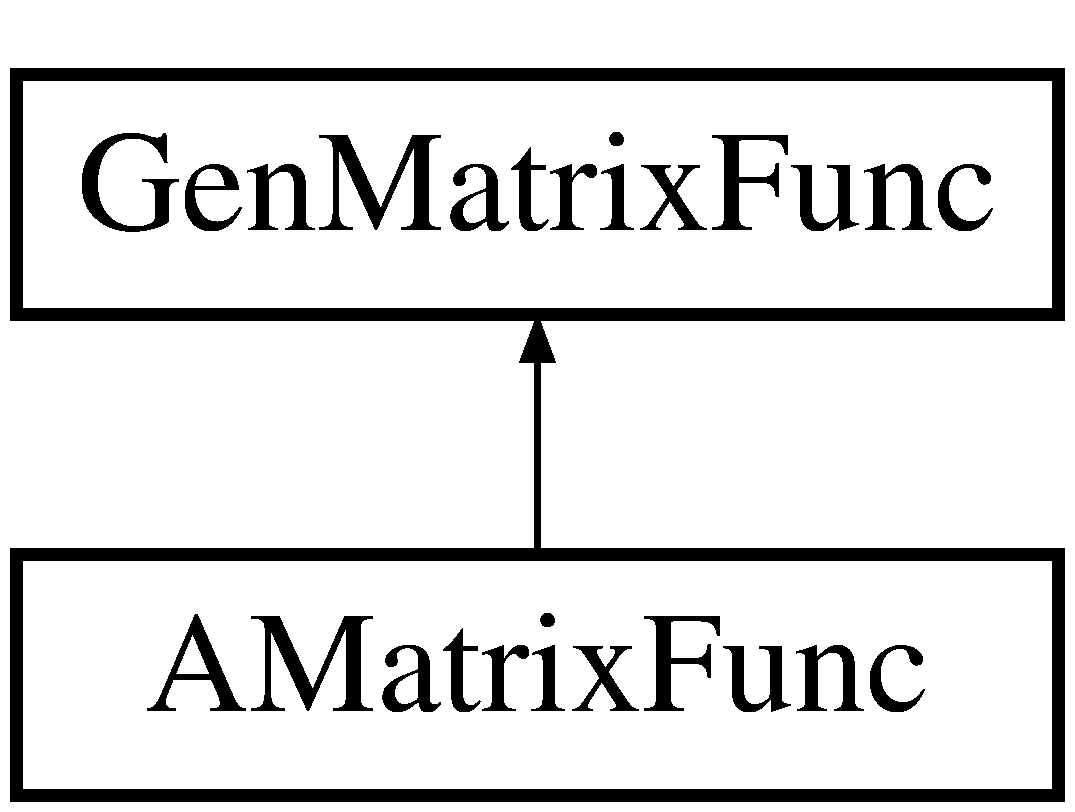
\includegraphics[height=2cm]{classAMatrixFunc}
\end{center}
\end{figure}
\subsection*{Public Member Functions}
\begin{CompactItemize}
\item 
\bf{AMatrix\-Func} (\bf{CNuc} $\ast$)
\item 
\bf{CNuc} $\ast$ \bf{compound} () const 
\item 
void \bf{Clear\-Matrices} ()
\item 
void \bf{Fill\-Matrices} (\bf{EPoint} $\ast$)
\item 
void \bf{Invert\-Matrices} ()
\item 
void \bf{Calculate\-TMatrix} (\bf{EPoint} $\ast$)
\item 
void \bf{Calculate\-Cross\-Section} ()
\item 
std::complex$<$ double $>$ \bf{Get\-AMatrix\-Element} (int, int, int) const 
\item 
std::vector$<$ std::vector$<$ std::complex$<$ double $>$ $>$ $>$ $\ast$ \bf{Get\-JSpec\-AInv\-Matrix} (int)
\item 
void \bf{Add\-AInv\-Matrix\-Element} (int, int, int, std::complex$<$ double $>$)
\item 
void \bf{Add\-AMatrix} (std::vector$<$ std::vector$<$ std::complex$<$ double $>$ $>$ $>$)
\end{CompactItemize}


\subsection{Detailed Description}
A function class to calculate the T-Matrix using the A-Matrix. 

The \doxyref{AMatrix\-Func}{p.}{classAMatrixFunc} function class calculates the T-Matrix for a given energy point using the compound nucleus object. The \doxyref{AMatrix\-Func}{p.}{classAMatrixFunc} class is a child class of \doxyref{Gen\-Matrix\-Func}{p.}{classGenMatrixFunc}, where the cross section is calculated from the T-Matrix. 



\subsection{Constructor \& Destructor Documentation}
\index{AMatrixFunc@{AMatrix\-Func}!AMatrixFunc@{AMatrixFunc}}
\index{AMatrixFunc@{AMatrixFunc}!AMatrixFunc@{AMatrix\-Func}}
\subsubsection{\setlength{\rightskip}{0pt plus 5cm}AMatrix\-Func::AMatrix\-Func (\bf{CNuc} $\ast$ {\em compound})}\label{classAMatrixFunc_c42c2ef591b731992ca551fe4f6be19f}


The \doxyref{AMatrix\-Func}{p.}{classAMatrixFunc} object is created with reference to a \doxyref{CNuc}{p.}{classCNuc} object. 

\subsection{Member Function Documentation}
\index{AMatrixFunc@{AMatrix\-Func}!AddAInvMatrixElement@{AddAInvMatrixElement}}
\index{AddAInvMatrixElement@{AddAInvMatrixElement}!AMatrixFunc@{AMatrix\-Func}}
\subsubsection{\setlength{\rightskip}{0pt plus 5cm}void AMatrix\-Func::Add\-AInv\-Matrix\-Element (int {\em j\-Group\-Num}, int {\em lambda\-Num}, int {\em mu\-Num}, std::complex$<$ double $>$ {\em a\-Matrix\-Element})}\label{classAMatrixFunc_fea5d08a7a9cbb7b57fc98398fe71093}


This function adds an inverse A-Matrix element specified by positions in the \doxyref{JGroup}{p.}{classJGroup} and \doxyref{ALevel}{p.}{classALevel} vectors. \index{AMatrixFunc@{AMatrix\-Func}!AddAMatrix@{AddAMatrix}}
\index{AddAMatrix@{AddAMatrix}!AMatrixFunc@{AMatrix\-Func}}
\subsubsection{\setlength{\rightskip}{0pt plus 5cm}void AMatrix\-Func::Add\-AMatrix (std::vector$<$ std::vector$<$ std::complex$<$ double $>$ $>$ $>$ {\em a\-Matrix})}\label{classAMatrixFunc_643bf6968600d248630cdcf3ccd3dd9e}


This function adds an entire A-Matrix to a vector. \index{AMatrixFunc@{AMatrix\-Func}!CalculateCrossSection@{CalculateCrossSection}}
\index{CalculateCrossSection@{CalculateCrossSection}!AMatrixFunc@{AMatrix\-Func}}
\subsubsection{\setlength{\rightskip}{0pt plus 5cm}void AMatrix\-Func::Calculate\-Cross\-Section ()}\label{classAMatrixFunc_b130caca8580e88892413d381e094499}


Instantiated in the parent class. \index{AMatrixFunc@{AMatrix\-Func}!CalculateTMatrix@{CalculateTMatrix}}
\index{CalculateTMatrix@{CalculateTMatrix}!AMatrixFunc@{AMatrix\-Func}}
\subsubsection{\setlength{\rightskip}{0pt plus 5cm}void AMatrix\-Func::Calculate\-TMatrix (\bf{EPoint} $\ast$ {\em point})\hspace{0.3cm}{\tt  [virtual]}}\label{classAMatrixFunc_6a4b63537f9c4716afc2cf03874ae2f3}


This function calculates the T-Matrix for each reaction pathway based on the A-Matrix. 

Implements \bf{Gen\-Matrix\-Func} \doxyref{p.}{classGenMatrixFunc_f89bf73a0a2f230c2187947520c1f360}.\index{AMatrixFunc@{AMatrix\-Func}!ClearMatrices@{ClearMatrices}}
\index{ClearMatrices@{ClearMatrices}!AMatrixFunc@{AMatrix\-Func}}
\subsubsection{\setlength{\rightskip}{0pt plus 5cm}void AMatrix\-Func::Clear\-Matrices ()\hspace{0.3cm}{\tt  [virtual]}}\label{classAMatrixFunc_9fa5a3ed65bf42990f74fe4cb482eb02}


Clears all matrices associated with the \doxyref{AMatrix\-Func}{p.}{classAMatrixFunc} object. 

Implements \bf{Gen\-Matrix\-Func} \doxyref{p.}{classGenMatrixFunc_41a9098087eac97b9c7de7aee82fa3d8}.\index{AMatrixFunc@{AMatrix\-Func}!compound@{compound}}
\index{compound@{compound}!AMatrixFunc@{AMatrix\-Func}}
\subsubsection{\setlength{\rightskip}{0pt plus 5cm}\bf{CNuc}$\ast$ AMatrix\-Func::compound () const\hspace{0.3cm}{\tt  [inline, virtual]}}\label{classAMatrixFunc_edf46d126dcf0748e0325bf39cbedde9}


Returns a pointer to the compound nucleus object. 

Implements \bf{Gen\-Matrix\-Func} \doxyref{p.}{classGenMatrixFunc_12603673326e93fb80d8db05fad085de}.\index{AMatrixFunc@{AMatrix\-Func}!FillMatrices@{FillMatrices}}
\index{FillMatrices@{FillMatrices}!AMatrixFunc@{AMatrix\-Func}}
\subsubsection{\setlength{\rightskip}{0pt plus 5cm}void AMatrix\-Func::Fill\-Matrices (\bf{EPoint} $\ast$ {\em point})\hspace{0.3cm}{\tt  [virtual]}}\label{classAMatrixFunc_953efa806622175437e1207c8fcda61c}


This function creates the inverted A-Matrix from the parameters in the \doxyref{CNuc}{p.}{classCNuc} object. 

Implements \bf{Gen\-Matrix\-Func} \doxyref{p.}{classGenMatrixFunc_0ce6fcce1afbd13bfdb753fcdfbe196c}.\index{AMatrixFunc@{AMatrix\-Func}!GetAMatrixElement@{GetAMatrixElement}}
\index{GetAMatrixElement@{GetAMatrixElement}!AMatrixFunc@{AMatrix\-Func}}
\subsubsection{\setlength{\rightskip}{0pt plus 5cm}std::complex$<$ double $>$ AMatrix\-Func::Get\-AMatrix\-Element (int {\em j\-Group\-Num}, int {\em lambda\-Num}, int {\em mu\-Num}) const}\label{classAMatrixFunc_d44334b6774b866cd1f181c6d0ebc2f3}


Returns an A-Matrix element specified by positions in the \doxyref{JGroup}{p.}{classJGroup} and \doxyref{ALevel}{p.}{classALevel} vectors. \index{AMatrixFunc@{AMatrix\-Func}!GetJSpecAInvMatrix@{GetJSpecAInvMatrix}}
\index{GetJSpecAInvMatrix@{GetJSpecAInvMatrix}!AMatrixFunc@{AMatrix\-Func}}
\subsubsection{\setlength{\rightskip}{0pt plus 5cm}std::vector$<$ std::vector$<$ std::complex$<$ double $>$ $>$ $>$ $\ast$ AMatrix\-Func::Get\-JSpec\-AInv\-Matrix (int {\em j\-Group\-Num})}\label{classAMatrixFunc_468bde19a3f3ddcdfef565f6a99597f3}


Returns a pointer to an entire A-Matrix specified by a position in the \doxyref{JGroup}{p.}{classJGroup} vector. \index{AMatrixFunc@{AMatrix\-Func}!InvertMatrices@{InvertMatrices}}
\index{InvertMatrices@{InvertMatrices}!AMatrixFunc@{AMatrix\-Func}}
\subsubsection{\setlength{\rightskip}{0pt plus 5cm}void AMatrix\-Func::Invert\-Matrices ()\hspace{0.3cm}{\tt  [virtual]}}\label{classAMatrixFunc_cf45883ba4979a32596214d356b48766}


This function inverts the inverse A-Matrix to yeild the A-Matrix. 

Implements \bf{Gen\-Matrix\-Func} \doxyref{p.}{classGenMatrixFunc_2dbfafa4c608ad5c1b27db7684f8f839}.

The documentation for this class was generated from the following files:\begin{CompactItemize}
\item 
azure\_\-v2/include/AMatrix\-Func.h\item 
azure\_\-v2/src/AMatrix\-Func.cpp\end{CompactItemize}

\section{AZURECalc Class Reference}
\label{classAZURECalc}\index{AZURECalc@{AZURECalc}}
A function class to perform the calculation of the chi-squared value.  


{\tt \#include $<$AZURECalc.h$>$}

\subsection*{Public Member Functions}
\begin{CompactItemize}
\item 
\bf{AZURECalc} (\bf{EData} $\ast$data, \bf{CNuc} $\ast$compound, const \bf{Config} \&configure)
\item 
virtual double \bf{Up} () const 
\item 
virtual double \bf{operator()} (const std::vector$<$ double $>$ \&) const 
\item 
const \bf{Config} \& \bf{configure} () const 
\item 
\bf{EData} $\ast$ \bf{data} () const 
\item 
\bf{CNuc} $\ast$ \bf{compound} () const 
\item 
void \bf{Set\-Error\-Def} (double def)
\end{CompactItemize}


\subsection{Detailed Description}
A function class to perform the calculation of the chi-squared value. 

The \doxyref{AZURECalc}{p.}{classAZURECalc} function class calculates the cross section based on a parameter set for all available data, and returns a chi-squared value. This function class is what Minuit calls repeatedly during the fitting process to perform the minimization. 



\subsection{Constructor \& Destructor Documentation}
\index{AZURECalc@{AZURECalc}!AZURECalc@{AZURECalc}}
\index{AZURECalc@{AZURECalc}!AZURECalc@{AZURECalc}}
\subsubsection{\setlength{\rightskip}{0pt plus 5cm}AZURECalc::AZURECalc (\bf{EData} $\ast$ {\em data}, \bf{CNuc} $\ast$ {\em compound}, const \bf{Config} \& {\em configure})\hspace{0.3cm}{\tt  [inline]}}\label{classAZURECalc_b8b3ce17df63a6925b28f62fb99034cc}


The \doxyref{AZURECalc}{p.}{classAZURECalc} object is created with reference to an \doxyref{EData}{p.}{classEData} and \doxyref{CNuc}{p.}{classCNuc} object. . The runtime configurations are also passed through a \doxyref{Config}{p.}{structConfig} structure. 

\subsection{Member Function Documentation}
\index{AZURECalc@{AZURECalc}!compound@{compound}}
\index{compound@{compound}!AZURECalc@{AZURECalc}}
\subsubsection{\setlength{\rightskip}{0pt plus 5cm}\bf{CNuc}$\ast$ AZURECalc::compound () const\hspace{0.3cm}{\tt  [inline]}}\label{classAZURECalc_d4f5088fe96da5f3de2d8caf0b1b2657}


Returns a pointer to the \doxyref{CNuc}{p.}{classCNuc} object. \index{AZURECalc@{AZURECalc}!configure@{configure}}
\index{configure@{configure}!AZURECalc@{AZURECalc}}
\subsubsection{\setlength{\rightskip}{0pt plus 5cm}const \bf{Config}\& AZURECalc::configure () const\hspace{0.3cm}{\tt  [inline]}}\label{classAZURECalc_9a4c7c6c8ebdcd93c9d3ec385c889c70}


Returns a reference to the \doxyref{Config}{p.}{structConfig} structure. \index{AZURECalc@{AZURECalc}!data@{data}}
\index{data@{data}!AZURECalc@{AZURECalc}}
\subsubsection{\setlength{\rightskip}{0pt plus 5cm}\bf{EData}$\ast$ AZURECalc::data () const\hspace{0.3cm}{\tt  [inline]}}\label{classAZURECalc_7e21612a13bd791c91608b4ca967beaa}


Returns a pointer to the \doxyref{EData}{p.}{classEData} object. \index{AZURECalc@{AZURECalc}!operator()@{operator()}}
\index{operator()@{operator()}!AZURECalc@{AZURECalc}}
\subsubsection{\setlength{\rightskip}{0pt plus 5cm}double AZURECalc::operator() (const std::vector$<$ double $>$ \&) const\hspace{0.3cm}{\tt  [virtual]}}\label{classAZURECalc_9f8d9d22ecc213b7f69e0bfc168fbb02}


Overloaded operator to make the class instance callable as a function. A Minuit parameter array is passed as the dependent variable. The function returns the total chi-squared value. \index{AZURECalc@{AZURECalc}!SetErrorDef@{SetErrorDef}}
\index{SetErrorDef@{SetErrorDef}!AZURECalc@{AZURECalc}}
\subsubsection{\setlength{\rightskip}{0pt plus 5cm}void AZURECalc::Set\-Error\-Def (double {\em def})\hspace{0.3cm}{\tt  [inline]}}\label{classAZURECalc_5b7e60b3fdd96f2b189bcc0a2ff287c8}


See Minuit2 documentation for an explanation of this function. \index{AZURECalc@{AZURECalc}!Up@{Up}}
\index{Up@{Up}!AZURECalc@{AZURECalc}}
\subsubsection{\setlength{\rightskip}{0pt plus 5cm}virtual double AZURECalc::Up () const\hspace{0.3cm}{\tt  [inline, virtual]}}\label{classAZURECalc_d907064e772f88dc45f24306ebfb53c7}


See Minuit2 documentation for an explanation of this function. 

The documentation for this class was generated from the following files:\begin{CompactItemize}
\item 
azure\_\-v2/include/AZURECalc.h\item 
azure\_\-v2/src/AZURECalc.cpp\item 
azure\_\-v2/src/AZURECalc\_\-thread.cpp\end{CompactItemize}

\section{AZUREFBuffer Class Reference}
\label{classAZUREFBuffer}\index{AZUREFBuffer@{AZUREFBuffer}}
A container class for a pointer to a file buffer.  


{\tt \#include $<$AZUREFBuffer.h$>$}

\subsection*{Public Member Functions}
\begin{CompactItemize}
\item 
\bf{AZUREFBuffer} (int entrance\-Key, int exit\-Key, std::string outputdir)
\item 
\bf{$\sim$AZUREFBuffer} ()
\item 
int \bf{Get\-Entrance\-Key} () const 
\item 
int \bf{Get\-Exit\-Key} () const 
\item 
std::filebuf $\ast$ \bf{Get\-FBuffer} ()
\end{CompactItemize}


\subsection{Detailed Description}
A container class for a pointer to a file buffer. 

The \doxyref{AZUREFBuffer}{p.}{classAZUREFBuffer} class contains a pointer to an acutal file buffer, as well as the entrance and exit pair keys to which the file buffer corresponds. 



\subsection{Constructor \& Destructor Documentation}
\index{AZUREFBuffer@{AZUREFBuffer}!AZUREFBuffer@{AZUREFBuffer}}
\index{AZUREFBuffer@{AZUREFBuffer}!AZUREFBuffer@{AZUREFBuffer}}
\subsubsection{\setlength{\rightskip}{0pt plus 5cm}AZUREFBuffer::AZUREFBuffer (int {\em entrance\-Key}, int {\em exit\-Key}, std::string {\em outputdir})\hspace{0.3cm}{\tt  [inline]}}\label{classAZUREFBuffer_9c1cb6118101b673553e23800365124f}


The \doxyref{AZUREFBuffer}{p.}{classAZUREFBuffer} object is created with an entrance and exit pair key, as well as an output directory. The filename is determined, and a file buffer is created with that filename. \index{AZUREFBuffer@{AZUREFBuffer}!~AZUREFBuffer@{$\sim$AZUREFBuffer}}
\index{~AZUREFBuffer@{$\sim$AZUREFBuffer}!AZUREFBuffer@{AZUREFBuffer}}
\subsubsection{\setlength{\rightskip}{0pt plus 5cm}AZUREFBuffer::$\sim$AZUREFBuffer ()\hspace{0.3cm}{\tt  [inline]}}\label{classAZUREFBuffer_de8225c83f2fbd725207261409c2d582}


The file buffer is closed and destroyed with the instance of \doxyref{AZUREFBuffer}{p.}{classAZUREFBuffer}. 

\subsection{Member Function Documentation}
\index{AZUREFBuffer@{AZUREFBuffer}!GetEntranceKey@{GetEntranceKey}}
\index{GetEntranceKey@{GetEntranceKey}!AZUREFBuffer@{AZUREFBuffer}}
\subsubsection{\setlength{\rightskip}{0pt plus 5cm}int AZUREFBuffer::Get\-Entrance\-Key () const\hspace{0.3cm}{\tt  [inline]}}\label{classAZUREFBuffer_4e017969da396973cc0b5b8f7bc9b021}


Returns the entrance pair key of the object. \index{AZUREFBuffer@{AZUREFBuffer}!GetExitKey@{GetExitKey}}
\index{GetExitKey@{GetExitKey}!AZUREFBuffer@{AZUREFBuffer}}
\subsubsection{\setlength{\rightskip}{0pt plus 5cm}int AZUREFBuffer::Get\-Exit\-Key () const\hspace{0.3cm}{\tt  [inline]}}\label{classAZUREFBuffer_1df7cc6cf2e2e9c44cf9f4fb42b2698b}


Returns the exit pair key of the object. \index{AZUREFBuffer@{AZUREFBuffer}!GetFBuffer@{GetFBuffer}}
\index{GetFBuffer@{GetFBuffer}!AZUREFBuffer@{AZUREFBuffer}}
\subsubsection{\setlength{\rightskip}{0pt plus 5cm}std::filebuf$\ast$ AZUREFBuffer::Get\-FBuffer ()\hspace{0.3cm}{\tt  [inline]}}\label{classAZUREFBuffer_b019c8d8718aaeb374aaa0552c64ba0b}


Returns a pointer to the corresponding file buffer. 

The documentation for this class was generated from the following file:\begin{CompactItemize}
\item 
azure\_\-v2/include/AZUREFBuffer.h\end{CompactItemize}

\section{AZUREMain Class Reference}
\label{classAZUREMain}\index{AZUREMain@{AZUREMain}}
The top-level AZURE function class.  


{\tt \#include $<$AZUREMain.h$>$}

\subsection*{Public Member Functions}
\begin{CompactItemize}
\item 
\bf{AZUREMain} (const \bf{Config} \&configure)
\item 
\bf{$\sim$AZUREMain} ()
\item 
int \bf{operator()} ()
\item 
const \bf{Config} \& \bf{configure} () const 
\item 
\bf{CNuc} $\ast$ \bf{compound} () const 
\item 
\bf{EData} $\ast$ \bf{data} () const 
\end{CompactItemize}


\subsection{Detailed Description}
The top-level AZURE function class. 

The \doxyref{AZUREMain}{p.}{classAZUREMain} function class is the top level function class in the AZURE package. It is called directly from them main() using the configuration parameters read from the runtime file as well as from the command shell prompt. 



\subsection{Constructor \& Destructor Documentation}
\index{AZUREMain@{AZUREMain}!AZUREMain@{AZUREMain}}
\index{AZUREMain@{AZUREMain}!AZUREMain@{AZUREMain}}
\subsubsection{\setlength{\rightskip}{0pt plus 5cm}AZUREMain::AZUREMain (const \bf{Config} \& {\em configure})\hspace{0.3cm}{\tt  [inline]}}\label{classAZUREMain_5ad95cc68ecd0e65c75aca3685a70411}


The \doxyref{AZUREMain}{p.}{classAZUREMain} function class is created using a \doxyref{Config}{p.}{structConfig} structure. New \doxyref{CNuc}{p.}{classCNuc} and \doxyref{EData}{p.}{classEData} objects are created at initialization of an \doxyref{AZUREMain}{p.}{classAZUREMain} object. \index{AZUREMain@{AZUREMain}!~AZUREMain@{$\sim$AZUREMain}}
\index{~AZUREMain@{$\sim$AZUREMain}!AZUREMain@{AZUREMain}}
\subsubsection{\setlength{\rightskip}{0pt plus 5cm}AZUREMain::$\sim$AZUREMain ()\hspace{0.3cm}{\tt  [inline]}}\label{classAZUREMain_7dcd41c3bd2f5dabcd352a80a7c912dc}


The \doxyref{CNuc}{p.}{classCNuc} and \doxyref{EData}{p.}{classEData} objects are destroyed with the \doxyref{AZUREMain}{p.}{classAZUREMain} instance. 

\subsection{Member Function Documentation}
\index{AZUREMain@{AZUREMain}!compound@{compound}}
\index{compound@{compound}!AZUREMain@{AZUREMain}}
\subsubsection{\setlength{\rightskip}{0pt plus 5cm}\bf{CNuc}$\ast$ AZUREMain::compound () const\hspace{0.3cm}{\tt  [inline]}}\label{classAZUREMain_0d14eda656b4a51bac4ee6ee8fcbab69}


Returns a pointer to the \doxyref{CNuc}{p.}{classCNuc} object. \index{AZUREMain@{AZUREMain}!configure@{configure}}
\index{configure@{configure}!AZUREMain@{AZUREMain}}
\subsubsection{\setlength{\rightskip}{0pt plus 5cm}const \bf{Config}\& AZUREMain::configure () const\hspace{0.3cm}{\tt  [inline]}}\label{classAZUREMain_91c819dc90dcf36600575859201c7725}


Returns a reference to the \doxyref{Config}{p.}{structConfig} structure. \index{AZUREMain@{AZUREMain}!data@{data}}
\index{data@{data}!AZUREMain@{AZUREMain}}
\subsubsection{\setlength{\rightskip}{0pt plus 5cm}\bf{EData}$\ast$ AZUREMain::data () const\hspace{0.3cm}{\tt  [inline]}}\label{classAZUREMain_a0990ed1fba1e4d698f753a637b4e665}


Returns a pointer to the \doxyref{EData}{p.}{classEData} object. \index{AZUREMain@{AZUREMain}!operator()@{operator()}}
\index{operator()@{operator()}!AZUREMain@{AZUREMain}}
\subsubsection{\setlength{\rightskip}{0pt plus 5cm}int AZUREMain::operator() ()}\label{classAZUREMain_6dd46db1e65d08347b1accbf88267495}


The parenthesis operator is defined so the instance of \doxyref{AZUREMain}{p.}{classAZUREMain} can be called as a function. This executes AZURE against the configuration parameters. 

The documentation for this class was generated from the following files:\begin{CompactItemize}
\item 
azure\_\-v2/include/AZUREMain.h\item 
azure\_\-v2/src/AZUREMain.cpp\end{CompactItemize}

\section{AZUREOutput Class Reference}
\label{classAZUREOutput}\index{AZUREOutput@{AZUREOutput}}
A class to assist in writing AZURE output files.  


{\tt \#include $<$AZUREOutput.h$>$}

\subsection*{Public Member Functions}
\begin{CompactItemize}
\item 
\bf{AZUREOutput} (std::string)
\item 
\bf{$\sim$AZUREOutput} ()
\item 
std::filebuf $\ast$ \bf{operator()} (int, int)
\item 
int \bf{Num\-AZUREFBuffers} () const 
\item 
int \bf{Is\-AZUREFBuffer} (int, int)
\item 
std::string \bf{Get\-Output\-Dir} () const 
\item 
void \bf{Add\-AZUREFBuffer} (\bf{AZUREFBuffer} $\ast$)
\item 
\bf{AZUREFBuffer} $\ast$ \bf{Get\-AZUREFBuffer} (int)
\end{CompactItemize}


\subsection{Detailed Description}
A class to assist in writing AZURE output files. 

The \doxyref{EData::Write\-Output\-Files}{p.}{classEData_16f9f5417f14467045eabea4b93d288f} function simply loops over all \doxyref{ESegment}{p.}{classESegment} and \doxyref{EPoint}{p.}{classEPoint} objects when writing the output of an AZURE calculation. To ensure that all output for a given entrance and exit pair combination is written to a single file, the \doxyref{AZUREOutput}{p.}{classAZUREOutput} class is used. The \doxyref{AZUREOutput}{p.}{classAZUREOutput} object is a container for a vector of \doxyref{AZUREFBuffer}{p.}{classAZUREFBuffer} objects. 



\subsection{Constructor \& Destructor Documentation}
\index{AZUREOutput@{AZUREOutput}!AZUREOutput@{AZUREOutput}}
\index{AZUREOutput@{AZUREOutput}!AZUREOutput@{AZUREOutput}}
\subsubsection{\setlength{\rightskip}{0pt plus 5cm}AZUREOutput::AZUREOutput (std::string {\em outputdir})}\label{classAZUREOutput_f1c62484313c9697ea274794316fecd7}


The \doxyref{AZUREOutput}{p.}{classAZUREOutput} object is created with reference to an output directory. \index{AZUREOutput@{AZUREOutput}!~AZUREOutput@{$\sim$AZUREOutput}}
\index{~AZUREOutput@{$\sim$AZUREOutput}!AZUREOutput@{AZUREOutput}}
\subsubsection{\setlength{\rightskip}{0pt plus 5cm}AZUREOutput::$\sim$AZUREOutput ()}\label{classAZUREOutput_1de72879a35e492afbadaca832025238}


On destruction of the \doxyref{AZUREOutput}{p.}{classAZUREOutput} instance, each \doxyref{AZUREFBuffer}{p.}{classAZUREFBuffer} object is also destroyed. 

\subsection{Member Function Documentation}
\index{AZUREOutput@{AZUREOutput}!AddAZUREFBuffer@{AddAZUREFBuffer}}
\index{AddAZUREFBuffer@{AddAZUREFBuffer}!AZUREOutput@{AZUREOutput}}
\subsubsection{\setlength{\rightskip}{0pt plus 5cm}void AZUREOutput::Add\-AZUREFBuffer (\bf{AZUREFBuffer} $\ast$ {\em azure\-FBuffer})}\label{classAZUREOutput_77b2179c2b51d607552b281e07cb8c5a}


Adds a pointer to an \doxyref{AZUREFBuffer}{p.}{classAZUREFBuffer} object to the vector. \index{AZUREOutput@{AZUREOutput}!GetAZUREFBuffer@{GetAZUREFBuffer}}
\index{GetAZUREFBuffer@{GetAZUREFBuffer}!AZUREOutput@{AZUREOutput}}
\subsubsection{\setlength{\rightskip}{0pt plus 5cm}\bf{AZUREFBuffer} $\ast$ AZUREOutput::Get\-AZUREFBuffer (int {\em f\-Buffer\-Num})}\label{classAZUREOutput_c7130df2eb622c234419ab9b5f8c8346}


Returns a pointer to the \doxyref{AZUREFBuffer}{p.}{classAZUREFBuffer} object specified by a position in the vector. \index{AZUREOutput@{AZUREOutput}!GetOutputDir@{GetOutputDir}}
\index{GetOutputDir@{GetOutputDir}!AZUREOutput@{AZUREOutput}}
\subsubsection{\setlength{\rightskip}{0pt plus 5cm}std::string AZUREOutput::Get\-Output\-Dir () const}\label{classAZUREOutput_51e4ce503deaddf42589961685d2b095}


Returns the output directory for the \doxyref{AZUREOutput}{p.}{classAZUREOutput} object. \index{AZUREOutput@{AZUREOutput}!IsAZUREFBuffer@{IsAZUREFBuffer}}
\index{IsAZUREFBuffer@{IsAZUREFBuffer}!AZUREOutput@{AZUREOutput}}
\subsubsection{\setlength{\rightskip}{0pt plus 5cm}int AZUREOutput::Is\-AZUREFBuffer (int {\em entrance\-Key}, int {\em exit\-Key})}\label{classAZUREOutput_8e4b2e9df5d4f2455c13631990a7624a}


Tests if a pointer to an \doxyref{AZUREFBuffer}{p.}{classAZUREFBuffer} object corresponding to the specified entrance and exit keys exists in the vector. If such a pointer exists, the position in the vector is returned. Otherwise, the function returns 0. \index{AZUREOutput@{AZUREOutput}!NumAZUREFBuffers@{NumAZUREFBuffers}}
\index{NumAZUREFBuffers@{NumAZUREFBuffers}!AZUREOutput@{AZUREOutput}}
\subsubsection{\setlength{\rightskip}{0pt plus 5cm}int AZUREOutput::Num\-AZUREFBuffers () const}\label{classAZUREOutput_86b3e62ba655f65582918bd3714d9e17}


Returns the number of pointers to \doxyref{AZUREFBuffer}{p.}{classAZUREFBuffer} objects stored in the vector. \index{AZUREOutput@{AZUREOutput}!operator()@{operator()}}
\index{operator()@{operator()}!AZUREOutput@{AZUREOutput}}
\subsubsection{\setlength{\rightskip}{0pt plus 5cm}std::filebuf $\ast$ AZUREOutput::operator() (int {\em entrance\-Key}, int {\em exit\-Key})}\label{classAZUREOutput_67885c872f33b61273b235e818248a60}


The parenthesis operator is defined so that the instance of \doxyref{AZUREOutput}{p.}{classAZUREOutput} can be called as a function. The instance is called using a reference to an entrance and exit pair key combination. The function tests if there is a pointer to an \doxyref{AZUREFBuffer}{p.}{classAZUREFBuffer} object in a vector. If such a pointer exists, the pointer to the actual file buffer contained in the corresponding \doxyref{AZUREFBuffer}{p.}{classAZUREFBuffer} object is returned. Otherwise, a new \doxyref{AZUREFBuffer}{p.}{classAZUREFBuffer} object is created with the entrance and exit key, a pointer to that object is stored in a vector, and the pointer to the actual new file buffer is returned. 

The documentation for this class was generated from the following files:\begin{CompactItemize}
\item 
azure\_\-v2/include/AZUREOutput.h\item 
azure\_\-v2/src/AZUREOutput.cpp\end{CompactItemize}

\section{CNuc Class Reference}
\label{classCNuc}\index{CNuc@{CNuc}}
An AZURE compound nucleus.  


{\tt \#include $<$CNuc.h$>$}

\subsection*{Public Member Functions}
\begin{CompactItemize}
\item 
bool \bf{Is\-Pair\-Key} (int)
\item 
int \bf{Num\-Pairs} () const 
\item 
int \bf{Num\-JGroups} () const 
\item 
int \bf{Is\-Pair} (\bf{PPair})
\item 
int \bf{Is\-JGroup} (\bf{JGroup})
\item 
int \bf{Get\-Pair\-Num\-From\-Key} (int)
\item 
int \bf{Fill} (const \bf{Config} \&)
\item 
int \bf{Read\-ECFile} (std::string)
\item 
int \bf{Get\-Max\-LValue} () const 
\item 
void \bf{Initialize} (const \bf{Config} \&)
\item 
void \bf{Add\-Pair} (\bf{PPair})
\item 
void \bf{Add\-JGroup} (\bf{JGroup})
\item 
void \bf{Print\-Nuc} (const \bf{Config} \&)
\item 
void \bf{Transform\-In} (bool)
\item 
void \bf{Sort\-Pathways} ()
\item 
void \bf{Print\-Pathways} (const \bf{Config} \&)
\item 
void \bf{Calc\-Boundary\-Conditions} ()
\item 
void \bf{Print\-Boundary\-Conditions} (const \bf{Config} \&)
\item 
void \bf{Calc\-Angular\-Dists} (int)
\item 
void \bf{Print\-Angular\-Dists} (const \bf{Config} \&)
\item 
void \bf{Fill\-Mn\-Params} (ROOT::Minuit2::Mn\-User\-Parameters \&)
\item 
void \bf{Fill\-Compound\-From\-Params} (const std::vector$<$ double $>$ \&)
\item 
void \bf{Transform\-Out} (bool)
\item 
void \bf{Print\-Transform\-Params} (std::string)
\item 
void \bf{Set\-Max\-LValue} (int)
\item 
std::complex$<$ double $>$ \bf{Calc\-External\-Width} (\bf{JGroup} $\ast$, \bf{ALevel} $\ast$, \bf{AChannel} $\ast$, bool)
\item 
\bf{PPair} $\ast$ \bf{Get\-Pair} (int)
\item 
\bf{JGroup} $\ast$ \bf{Get\-JGroup} (int)
\end{CompactItemize}


\subsection{Detailed Description}
An AZURE compound nucleus. 

The compound nucleus is the fundamental concept of R-Matrix theory. As such, the \doxyref{CNuc}{p.}{classCNuc} object in AZURE is the top level container object for all structure and reaction objects. Specifically, the \doxyref{CNuc}{p.}{classCNuc} object is the container object for vectors of \doxyref{PPair}{p.}{classPPair} and \doxyref{JGroup}{p.}{classJGroup} objects, within which all other nuclear data objects are contained. 



\subsection{Member Function Documentation}
\index{CNuc@{CNuc}!AddJGroup@{AddJGroup}}
\index{AddJGroup@{AddJGroup}!CNuc@{CNuc}}
\subsubsection{\setlength{\rightskip}{0pt plus 5cm}void CNuc::Add\-JGroup (\bf{JGroup} {\em j\-Group})}\label{classCNuc_7be7478265d55c961e612fcccf8d090c}


Adds a $ J^\pi $ group to the \doxyref{JGroup}{p.}{classJGroup} vector. \index{CNuc@{CNuc}!AddPair@{AddPair}}
\index{AddPair@{AddPair}!CNuc@{CNuc}}
\subsubsection{\setlength{\rightskip}{0pt plus 5cm}void CNuc::Add\-Pair (\bf{PPair} {\em p\-Pair})}\label{classCNuc_390aacd60d2085b670bbbf398b6eaa2b}


Adds a particle pair to the \doxyref{PPair}{p.}{classPPair} vector. \index{CNuc@{CNuc}!CalcAngularDists@{CalcAngularDists}}
\index{CalcAngularDists@{CalcAngularDists}!CNuc@{CNuc}}
\subsubsection{\setlength{\rightskip}{0pt plus 5cm}void CNuc::Calc\-Angular\-Dists (int {\em max\-L})}\label{classCNuc_bcf47c81408527cea193e0871309cb94}


Creates and sorts the \doxyref{KLGroup}{p.}{classKLGroup} and \doxyref{Interference}{p.}{classInterference} objects and calculates the appropriate coefficients. \index{CNuc@{CNuc}!CalcBoundaryConditions@{CalcBoundaryConditions}}
\index{CalcBoundaryConditions@{CalcBoundaryConditions}!CNuc@{CNuc}}
\subsubsection{\setlength{\rightskip}{0pt plus 5cm}void CNuc::Calc\-Boundary\-Conditions ()}\label{classCNuc_a6336f4425d0722384e0449443363aed}


Calculates the boundary conditions. Boundary conditions for each channel are evaluated at the energy of the first level read from the nuclear input file in the $ J^\pi $ group. \index{CNuc@{CNuc}!CalcExternalWidth@{CalcExternalWidth}}
\index{CalcExternalWidth@{CalcExternalWidth}!CNuc@{CNuc}}
\subsubsection{\setlength{\rightskip}{0pt plus 5cm}std::complex$<$ double $>$ CNuc::Calc\-External\-Width (\bf{JGroup} $\ast$ {\em the\-JGroup}, \bf{ALevel} $\ast$ {\em the\-Level}, \bf{AChannel} $\ast$ {\em the\-Channel}, bool {\em is\-Initial})}\label{classCNuc_e861c737257f4dd9017c47b484311466}


Calculates the external reduced width amplitudes for a given channel. \index{CNuc@{CNuc}!Fill@{Fill}}
\index{Fill@{Fill}!CNuc@{CNuc}}
\subsubsection{\setlength{\rightskip}{0pt plus 5cm}int CNuc::Fill (const \bf{Config} \& {\em configure})}\label{classCNuc_f8aa43b72f1e947ba449b60477aa1af0}


Fills the compound nucleus object, and all nested objects, from data specified in the nuclear and external capture input files. Returns -1 if the files could not be read, and 0 if the files were read successfully. \index{CNuc@{CNuc}!FillCompoundFromParams@{FillCompoundFromParams}}
\index{FillCompoundFromParams@{FillCompoundFromParams}!CNuc@{CNuc}}
\subsubsection{\setlength{\rightskip}{0pt plus 5cm}void CNuc::Fill\-Compound\-From\-Params (const std::vector$<$ double $>$ \& {\em p})}\label{classCNuc_fb2a580c9c7c2c498e3931dd25e8477c}


Fills the \doxyref{CNuc}{p.}{classCNuc} object from the Minuit parameter array. \index{CNuc@{CNuc}!FillMnParams@{FillMnParams}}
\index{FillMnParams@{FillMnParams}!CNuc@{CNuc}}
\subsubsection{\setlength{\rightskip}{0pt plus 5cm}void CNuc::Fill\-Mn\-Params (ROOT::Minuit2::Mn\-User\-Parameters \& {\em p})}\label{classCNuc_c8b88fe6c69b2459eca3a3207d5535c7}


Fills the Minuit parameter array from initial values in the \doxyref{CNuc}{p.}{classCNuc} object. \index{CNuc@{CNuc}!GetJGroup@{GetJGroup}}
\index{GetJGroup@{GetJGroup}!CNuc@{CNuc}}
\subsubsection{\setlength{\rightskip}{0pt plus 5cm}\bf{JGroup} $\ast$ CNuc::Get\-JGroup (int {\em j\-Group\-Num})}\label{classCNuc_068bb372b99501e66374eb350fc4d190}


Returns a pointer to the $ J^\pi $ group specified by a position in the \doxyref{JGroup}{p.}{classJGroup} vector. \index{CNuc@{CNuc}!GetMaxLValue@{GetMaxLValue}}
\index{GetMaxLValue@{GetMaxLValue}!CNuc@{CNuc}}
\subsubsection{\setlength{\rightskip}{0pt plus 5cm}int CNuc::Get\-Max\-LValue () const}\label{classCNuc_b0648dfaa788bffae4e82aa40efc47a8}


Returns the maximum value of orbital angular momentum read from channels in the nuclear file. \index{CNuc@{CNuc}!GetPair@{GetPair}}
\index{GetPair@{GetPair}!CNuc@{CNuc}}
\subsubsection{\setlength{\rightskip}{0pt plus 5cm}\bf{PPair} $\ast$ CNuc::Get\-Pair (int {\em pair\-Num})}\label{classCNuc_7fb37f5014c5665a1f3308c290a92c42}


Returns a pointer to the particle pair specified by a position in the \doxyref{PPair}{p.}{classPPair} vector. \index{CNuc@{CNuc}!GetPairNumFromKey@{GetPairNumFromKey}}
\index{GetPairNumFromKey@{GetPairNumFromKey}!CNuc@{CNuc}}
\subsubsection{\setlength{\rightskip}{0pt plus 5cm}int CNuc::Get\-Pair\-Num\-From\-Key (int {\em key})}\label{classCNuc_3e0d50e25c672cad8fadda8a4d8901e2}


Returns the position of a particle pair in the \doxyref{PPair}{p.}{classPPair} vector based on the pair key. Pair keys are how particle pairs are specified in the setup files, but may not correspond to the position of the particle pair in the \doxyref{PPair}{p.}{classPPair} vector. If the pair exists, the position in the vector is returned. Otherwise, the function returns 0. \index{CNuc@{CNuc}!Initialize@{Initialize}}
\index{Initialize@{Initialize}!CNuc@{CNuc}}
\subsubsection{\setlength{\rightskip}{0pt plus 5cm}void CNuc::Initialize (const \bf{Config} \& {\em configure})}\label{classCNuc_fccbd40a44a87f16793e980a23462ca0}


Initializes the compound nucleus object. This includes calculating the boundary conditions, transforming from physical to formal parameters, creating and sorting all reaction pathways, and calculating angular interference contributions and coefficients. A \doxyref{CNuc}{p.}{classCNuc} object can only be initialized for use AFTER it is filled. \index{CNuc@{CNuc}!IsJGroup@{IsJGroup}}
\index{IsJGroup@{IsJGroup}!CNuc@{CNuc}}
\subsubsection{\setlength{\rightskip}{0pt plus 5cm}int CNuc::Is\-JGroup (\bf{JGroup} {\em j\-Group})}\label{classCNuc_9d9ba124e32ca1934074c0c751251a33}


Tests if a $ J^\pi $ group exists in the \doxyref{JGroup}{p.}{classJGroup} vector. If the group exists, the position in the vector is returned. Otherwise, the function returns 0. \index{CNuc@{CNuc}!IsPair@{IsPair}}
\index{IsPair@{IsPair}!CNuc@{CNuc}}
\subsubsection{\setlength{\rightskip}{0pt plus 5cm}int CNuc::Is\-Pair (\bf{PPair} {\em pair})}\label{classCNuc_d7b5063187be9801b508a0527ced3418}


Tests if a particle pair exists in the \doxyref{PPair}{p.}{classPPair} vector. If pair exists, the position in the vector is returned. Otherwise, the function returns 0. \index{CNuc@{CNuc}!IsPairKey@{IsPairKey}}
\index{IsPairKey@{IsPairKey}!CNuc@{CNuc}}
\subsubsection{\setlength{\rightskip}{0pt plus 5cm}bool CNuc::Is\-Pair\-Key (int {\em key})}\label{classCNuc_ecb3f3f19909b757cdf296aca2c7cce2}


Returns true if a specified pair key exists in the \doxyref{PPair}{p.}{classPPair} vector, otherwise returns false. \index{CNuc@{CNuc}!NumJGroups@{NumJGroups}}
\index{NumJGroups@{NumJGroups}!CNuc@{CNuc}}
\subsubsection{\setlength{\rightskip}{0pt plus 5cm}int CNuc::Num\-JGroups () const}\label{classCNuc_344de874c014309a034271e10717b294}


Returns the number of $ J^\pi $ groups in the \doxyref{JGroup}{p.}{classJGroup} vector. \index{CNuc@{CNuc}!NumPairs@{NumPairs}}
\index{NumPairs@{NumPairs}!CNuc@{CNuc}}
\subsubsection{\setlength{\rightskip}{0pt plus 5cm}int CNuc::Num\-Pairs () const}\label{classCNuc_ac2ec0aec61d69eea744429a2edb5ad3}


Returns the number of particle pairs in the \doxyref{PPair}{p.}{classPPair} vector. \index{CNuc@{CNuc}!PrintAngularDists@{PrintAngularDists}}
\index{PrintAngularDists@{PrintAngularDists}!CNuc@{CNuc}}
\subsubsection{\setlength{\rightskip}{0pt plus 5cm}void CNuc::Print\-Angular\-Dists (const \bf{Config} \& {\em configure})}\label{classCNuc_b3b79c3d036ce4848764eb4ff254b113}


Prints the \doxyref{KLGroup}{p.}{classKLGroup} and \doxyref{Interference}{p.}{classInterference} object structure as well as the calculated coefficients. \index{CNuc@{CNuc}!PrintBoundaryConditions@{PrintBoundaryConditions}}
\index{PrintBoundaryConditions@{PrintBoundaryConditions}!CNuc@{CNuc}}
\subsubsection{\setlength{\rightskip}{0pt plus 5cm}void CNuc::Print\-Boundary\-Conditions (const \bf{Config} \& {\em configure})}\label{classCNuc_bac694722056e8510f93d6a0d7678eca}


Prints the boundary conditions. \index{CNuc@{CNuc}!PrintNuc@{PrintNuc}}
\index{PrintNuc@{PrintNuc}!CNuc@{CNuc}}
\subsubsection{\setlength{\rightskip}{0pt plus 5cm}void CNuc::Print\-Nuc (const \bf{Config} \& {\em configure})}\label{classCNuc_f91b924fa9f7e9724524e0c9b54ba569}


Prints the initial structure of the compound nucleus object after filling but before initialization. This includes all particle pairs, $ J^\pi $ groups, levels and channels. \index{CNuc@{CNuc}!PrintPathways@{PrintPathways}}
\index{PrintPathways@{PrintPathways}!CNuc@{CNuc}}
\subsubsection{\setlength{\rightskip}{0pt plus 5cm}void CNuc::Print\-Pathways (const \bf{Config} \& {\em configure})}\label{classCNuc_f173934c8f4d0fc0037613e528212734}


Prints the internal and external reaction pathways. \index{CNuc@{CNuc}!PrintTransformParams@{PrintTransformParams}}
\index{PrintTransformParams@{PrintTransformParams}!CNuc@{CNuc}}
\subsubsection{\setlength{\rightskip}{0pt plus 5cm}void CNuc::Print\-Transform\-Params (std::string {\em outdir})}\label{classCNuc_d78b9acad3f919b1125eb21fa11a9bcb}


Writes the final transformed parameters to \char`\"{}parameters.out\char`\"{} file. \index{CNuc@{CNuc}!ReadECFile@{ReadECFile}}
\index{ReadECFile@{ReadECFile}!CNuc@{CNuc}}
\subsubsection{\setlength{\rightskip}{0pt plus 5cm}int CNuc::Read\-ECFile (std::string {\em ecfile})}\label{classCNuc_dafdafc0a00d00124d9f717be7062c3d}


Fills the \doxyref{ECLevel}{p.}{classECLevel} vector from information in the external capture file. Also tests if the final state for external capture exists from the nuclear file. If not, the state is created. \index{CNuc@{CNuc}!SetMaxLValue@{SetMaxLValue}}
\index{SetMaxLValue@{SetMaxLValue}!CNuc@{CNuc}}
\subsubsection{\setlength{\rightskip}{0pt plus 5cm}void CNuc::Set\-Max\-LValue (int {\em max\-L})}\label{classCNuc_fee1fd95dadb7bbecca8b594dd8efcbe}


Sets the maximum orbital angular momentum value read from the nuclear input file. \index{CNuc@{CNuc}!SortPathways@{SortPathways}}
\index{SortPathways@{SortPathways}!CNuc@{CNuc}}
\subsubsection{\setlength{\rightskip}{0pt plus 5cm}void CNuc::Sort\-Pathways ()}\label{classCNuc_0ffd0e170506343a5ee8961e7a288a7c}


Calculates internal and external reaction pathways. \index{CNuc@{CNuc}!TransformIn@{TransformIn}}
\index{TransformIn@{TransformIn}!CNuc@{CNuc}}
\subsubsection{\setlength{\rightskip}{0pt plus 5cm}void CNuc::Transform\-In (bool {\em is\-EC})}\label{classCNuc_b463495e80bacd62a5ab42a8bdecce7c}


Performs the initial parameter transformations from physical to formal parameters. \index{CNuc@{CNuc}!TransformOut@{TransformOut}}
\index{TransformOut@{TransformOut}!CNuc@{CNuc}}
\subsubsection{\setlength{\rightskip}{0pt plus 5cm}void CNuc::Transform\-Out (bool {\em is\-EC})}\label{classCNuc_4fc7bad8e5bf06233e57b8a4ca5c7572}


Performs the final parameter transformations from formal to physical parameters. 

The documentation for this class was generated from the following files:\begin{CompactItemize}
\item 
azure\_\-v2/include/CNuc.h\item 
azure\_\-v2/src/CNuc.cpp\end{CompactItemize}

\section{Config Struct Reference}
\label{structConfig}\index{Config@{Config}}
A configuration structure for AZURE.  


{\tt \#include $<$Config.h$>$}

\subsection*{Public Attributes}
\begin{CompactItemize}
\item 
std::string \bf{configfile}\label{structConfig_f3049a94f812691bde9bc978554215da}

\begin{CompactList}\small\item\em The runtime configuration file name. \item\end{CompactList}\item 
bool \bf{is\-AMatrix}\label{structConfig_9d4e0f3c8f825552f5dd8c0c64449a97}

\begin{CompactList}\small\item\em A boolean specifying if the calculation should use the A-Matrix. \item\end{CompactList}\item 
std::string \bf{nucfile}\label{structConfig_6d9d9f1b6bef23879b7786ae511b4bbd}

\begin{CompactList}\small\item\em The nuclear input file name. \item\end{CompactList}\item 
std::string \bf{ecfile}\label{structConfig_85061e48a6ce3f509bb17669ae66289a}

\begin{CompactList}\small\item\em The external capture input file name. \item\end{CompactList}\item 
std::string \bf{segfile}\label{structConfig_c4e0e3319befab323b74c88d1a258d54}

\begin{CompactList}\small\item\em The data segments input file name. \item\end{CompactList}\item 
std::string \bf{extrapfile}\label{structConfig_9a025c9c94905aa016118619f94d7987}

\begin{CompactList}\small\item\em The extrapolation segments input file name. \item\end{CompactList}\item 
std::string \bf{outputdir}\label{structConfig_5a9a0ab96e1f23a30cb84ed03bfaee3e}

\begin{CompactList}\small\item\em The path of the output directory. \item\end{CompactList}\item 
std::string \bf{paramfile}\label{structConfig_c2d0d1b72f0b982c7755945bc11861e2}

\begin{CompactList}\small\item\em The name of the parameters file from which to read. \item\end{CompactList}\item 
std::string \bf{integralsfile}\label{structConfig_21150f56337fcca22e646e7e8bea6866}

\begin{CompactList}\small\item\em The name of the external capture amplitudes file from which to read. \item\end{CompactList}\item 
std::string \bf{checkdir}\label{structConfig_d2f2c592b83f9bd10118783d361d4a71}

\begin{CompactList}\small\item\em The path of the check files directory. \item\end{CompactList}\item 
std::string \bf{checknucleus}\label{structConfig_9afb9dd5ed6162c9c927d557b8fc668a}

\begin{CompactList}\small\item\em The specifier for the compound nucleus check output (none, screen, or file). \item\end{CompactList}\item 
std::string \bf{checkpathways}\label{structConfig_49e88a1097c83390f021cb961880a1a7}

\begin{CompactList}\small\item\em The specifier for the reaction pathways check output (none, screen, or file). \item\end{CompactList}\item 
std::string \bf{checkdata}\label{structConfig_299034194ce320bd3533935026ff8c60}

\begin{CompactList}\small\item\em The specifier for the data check output (none, screen, or file). \item\end{CompactList}\item 
std::string \bf{checkpene}\label{structConfig_d48d741600270723fc98973ee2703e93}

\begin{CompactList}\small\item\em The specifier for the energy dependent quantities check output (none, screen, or file). \item\end{CompactList}\item 
std::string \bf{checklegpoly}\label{structConfig_5d1ebe763cfc03d9390e696d6ab295d3}

\begin{CompactList}\small\item\em The specifier for the Legendre polynomials check output (none, screen, or file). \item\end{CompactList}\item 
std::string \bf{checkboundcon}\label{structConfig_d1be72c446c83a263df84f2e52780f7c}

\begin{CompactList}\small\item\em The specifier for the boundary condition check output (none, screen, or file). \item\end{CompactList}\item 
std::string \bf{checkangdists}\label{structConfig_4439469c56f76f4031eb50d598422b45}

\begin{CompactList}\small\item\em The specifier for the angular coefficient check output (none, screen, or file). \item\end{CompactList}\item 
std::string \bf{checkcoulamp}\label{structConfig_073756c433f9ed2be30631a9724e3f24}

\begin{CompactList}\small\item\em The specifier for the Coulomb amplitudes check output (none, screen, or file). \item\end{CompactList}\item 
bool \bf{perform\-Fit}\label{structConfig_c1c5f7fd069e0739f3033b2e72a9af12}

\begin{CompactList}\small\item\em A boolean specifying if a fit should be performed. \item\end{CompactList}\item 
bool \bf{with\-Data}\label{structConfig_30bd25d4db7888eb513863703c0d090e}

\begin{CompactList}\small\item\em A boolean specifying if AZURE will be executed in data driven mode. \item\end{CompactList}\item 
bool \bf{old\-Parameters}\label{structConfig_9c07a2cd66a0e76b330d3ce21f7d03f1}

\begin{CompactList}\small\item\em A boolean specifying if initial parameters should be read from an external file. \item\end{CompactList}\item 
bool \bf{is\-EC}\label{structConfig_ded13b3cfe22fb5ef97c16e7d6b21e79}

\begin{CompactList}\small\item\em A boolean specifying if external capture will be included. \item\end{CompactList}\item 
bool \bf{old\-ECFile}\label{structConfig_64b2073e49312bd269ed6290764d92d2}

\begin{CompactList}\small\item\em A boolean specifying if the external capture amplitudes will be read from and external file. \item\end{CompactList}\item 
bool \bf{calc\-Rate}\label{structConfig_6f2837648252bdb0c92a2c4bcb365bc0}

\begin{CompactList}\small\item\em A boolean specifying if the reaction rate should be calculated. \item\end{CompactList}\item 
int \bf{rate\-Entrance\-Pair}\label{structConfig_b7be0f5b262206071db9a59bfaf26659}

\begin{CompactList}\small\item\em If a reaction rate is calculated, value indicates the entrance pair key. \item\end{CompactList}\item 
int \bf{rate\-Exit\-Pair}\label{structConfig_443086aa534c84f2ca499d5a9e8ce2e0}

\begin{CompactList}\small\item\em If a reaction rate is calculated, value indicates the exit pair key. \item\end{CompactList}\item 
double \bf{rate\-Min\-Temp}\label{structConfig_de4858c442059530d6693fcaba637422}

\begin{CompactList}\small\item\em If a reaction rate is calculated, value indicates the minimum temperature in GK. \item\end{CompactList}\item 
double \bf{rate\-Max\-Temp}\label{structConfig_a2eba1530b0c79f4ccd832d19d2022c8}

\begin{CompactList}\small\item\em If a reaction rate is calculated, value indicates the maximum temperature in GK. \item\end{CompactList}\item 
double \bf{rate\-Temp\-Step}\label{structConfig_0a35e5393e7025d9876b1120b8036376}

\begin{CompactList}\small\item\em If a reaction rate is calculated, value indicates the temperature step in GK. \item\end{CompactList}\end{CompactItemize}
\subsection*{Static Public Attributes}
\begin{CompactItemize}
\item 
static const int \bf{max\-LOrder} = 10\label{structConfig_e61ee372c6a694582ce5cfa760bcd4c7}

\begin{CompactList}\small\item\em A constant indicating the maximum order of the Legendre polynomials to calculate. \item\end{CompactList}\end{CompactItemize}


\subsection{Detailed Description}
A configuration structure for AZURE. 

The configuration structure is created from the runtime file passed to the AZURE executable, as well as the options specified in the command shell prompt. 



The documentation for this struct was generated from the following file:\begin{CompactItemize}
\item 
azure\_\-v2/include/Config.h\end{CompactItemize}

\section{Coul\-Func Class Reference}
\label{classCoulFunc}\index{CoulFunc@{CoulFunc}}
A function class to calculate Coulomb functions for positive energy channels.  


{\tt \#include $<$Coul\-Func.h$>$}

\subsection*{Public Member Functions}
\begin{CompactItemize}
\item 
\bf{Coul\-Func} (\bf{PPair} $\ast$p\-Pair)
\item 
int \bf{z1} () const 
\item 
int \bf{z2} () const 
\item 
double \bf{redmass} () const 
\item 
int \bf{l\-Last} () const 
\item 
double \bf{radius\-Last} () const 
\item 
double \bf{energy\-Last} () const 
\item 
\bf{Coul\-Waves} \bf{coul\-Last} () const 
\item 
void \bf{set\-Last} (int l\-Last, double r\-Last, double e\-Last, \bf{Coul\-Waves} coul\-Last)
\item 
\bf{Coul\-Waves} \bf{operator()} (int l, double radius, double energy)
\item 
double \bf{Penetrability} (int l, double radius, double energy)
\item 
double \bf{PEShift} (int l, double radius, double energy)
\item 
double \bf{PEShift\_\-d\-E} (int l, double radius, double energy)
\end{CompactItemize}


\subsection{Detailed Description}
A function class to calculate Coulomb functions for positive energy channels. 

The \doxyref{Coul\-Func}{p.}{classCoulFunc} function class calculates the solutions to the Coulomb equation, as well as other useful quantities such as shift functions and their energy derivative and penetrabilities. 



\subsection{Constructor \& Destructor Documentation}
\index{CoulFunc@{Coul\-Func}!CoulFunc@{CoulFunc}}
\index{CoulFunc@{CoulFunc}!CoulFunc@{Coul\-Func}}
\subsubsection{\setlength{\rightskip}{0pt plus 5cm}Coul\-Func::Coul\-Func (\bf{PPair} $\ast$ {\em p\-Pair})\hspace{0.3cm}{\tt  [inline]}}\label{classCoulFunc_e878bae1900e0365939ce5115f9ca8bc}


The \doxyref{Coul\-Func}{p.}{classCoulFunc} object is created with reference to a \doxyref{PPair}{p.}{classPPair} object. 

\subsection{Member Function Documentation}
\index{CoulFunc@{Coul\-Func}!coulLast@{coulLast}}
\index{coulLast@{coulLast}!CoulFunc@{Coul\-Func}}
\subsubsection{\setlength{\rightskip}{0pt plus 5cm}struct \bf{Coul\-Waves} Coul\-Func::coul\-Last () const\hspace{0.3cm}{\tt  [inline]}}\label{classCoulFunc_c983b0b5fb84cc2065cca446ad392a7f}


Returns the last Coulomb functions which were calculated. \index{CoulFunc@{Coul\-Func}!energyLast@{energyLast}}
\index{energyLast@{energyLast}!CoulFunc@{Coul\-Func}}
\subsubsection{\setlength{\rightskip}{0pt plus 5cm}double Coul\-Func::energy\-Last () const\hspace{0.3cm}{\tt  [inline]}}\label{classCoulFunc_e6857b43f747e15e3948592cb68331f9}


Returns the last energy value at which the Coulomb functions were calculated. \index{CoulFunc@{Coul\-Func}!lLast@{lLast}}
\index{lLast@{lLast}!CoulFunc@{Coul\-Func}}
\subsubsection{\setlength{\rightskip}{0pt plus 5cm}int Coul\-Func::l\-Last () const\hspace{0.3cm}{\tt  [inline]}}\label{classCoulFunc_f26580308c3aa3c6ed6d8010272e0cc3}


Returns the last orbital angular momentum value at which the Coulomb functions were calculated. \index{CoulFunc@{Coul\-Func}!operator()@{operator()}}
\index{operator()@{operator()}!CoulFunc@{Coul\-Func}}
\subsubsection{\setlength{\rightskip}{0pt plus 5cm}\bf{Coul\-Waves} Coul\-Func::operator() (int {\em l}, double {\em radius}, double {\em energy})\hspace{0.3cm}{\tt  [inline]}}\label{classCoulFunc_23e202634cf67ee8732a9e305f3705a0}


The parenthesis operator is defined to make the class instance callable as a function. The orbital angular momentum, radius, and energy in the center of mass system are the dependent variables. The function returns the Coulomb waves. \index{CoulFunc@{Coul\-Func}!Penetrability@{Penetrability}}
\index{Penetrability@{Penetrability}!CoulFunc@{Coul\-Func}}
\subsubsection{\setlength{\rightskip}{0pt plus 5cm}double Coul\-Func::Penetrability (int {\em l}, double {\em radius}, double {\em energy})\hspace{0.3cm}{\tt  [inline]}}\label{classCoulFunc_be6a89daab7d985fb953fe14df4eb11f}


Returns the penetrability as a function of orbital angular momentum, radius, and energy in the center of mass system. \index{CoulFunc@{Coul\-Func}!PEShift@{PEShift}}
\index{PEShift@{PEShift}!CoulFunc@{Coul\-Func}}
\subsubsection{\setlength{\rightskip}{0pt plus 5cm}double Coul\-Func::PEShift (int {\em l}, double {\em radius}, double {\em energy})\hspace{0.3cm}{\tt  [inline]}}\label{classCoulFunc_1a0c29890b64e7019597c75f3484f4b9}


Returns the positive energy shift function a function of orbital angular momentum, radius, and energy in the center of mass system. \index{CoulFunc@{Coul\-Func}!PEShift_dE@{PEShift\_\-dE}}
\index{PEShift_dE@{PEShift\_\-dE}!CoulFunc@{Coul\-Func}}
\subsubsection{\setlength{\rightskip}{0pt plus 5cm}double Coul\-Func::PEShift\_\-d\-E (int {\em l}, double {\em radius}, double {\em energy})\hspace{0.3cm}{\tt  [inline]}}\label{classCoulFunc_7ba887bc6179ecff449f26e4574898c3}


Returns the energy derivative of the shift function a function of orbital angular momentum, radius, and energy in the center of mass system. \index{CoulFunc@{Coul\-Func}!radiusLast@{radiusLast}}
\index{radiusLast@{radiusLast}!CoulFunc@{Coul\-Func}}
\subsubsection{\setlength{\rightskip}{0pt plus 5cm}double Coul\-Func::radius\-Last () const\hspace{0.3cm}{\tt  [inline]}}\label{classCoulFunc_294416dd0757533011ebfd56c9597739}


Returns the last radius value at which the Coulomb functions were calculated. \index{CoulFunc@{Coul\-Func}!redmass@{redmass}}
\index{redmass@{redmass}!CoulFunc@{Coul\-Func}}
\subsubsection{\setlength{\rightskip}{0pt plus 5cm}double Coul\-Func::redmass () const\hspace{0.3cm}{\tt  [inline]}}\label{classCoulFunc_75d3ef5760151219ef16c916db221a83}


Returns the reduced mass of the particle pair. \index{CoulFunc@{Coul\-Func}!setLast@{setLast}}
\index{setLast@{setLast}!CoulFunc@{Coul\-Func}}
\subsubsection{\setlength{\rightskip}{0pt plus 5cm}void Coul\-Func::set\-Last (int {\em l\-Last}, double {\em r\-Last}, double {\em e\-Last}, \bf{Coul\-Waves} {\em coul\-Last})\hspace{0.3cm}{\tt  [inline]}}\label{classCoulFunc_ce06981b17573c1b6d2ba5a7f0616a2c}


Sets the last calculated Coulomb waves and the values for which they were calculated. \index{CoulFunc@{Coul\-Func}!z1@{z1}}
\index{z1@{z1}!CoulFunc@{Coul\-Func}}
\subsubsection{\setlength{\rightskip}{0pt plus 5cm}int Coul\-Func::z1 () const\hspace{0.3cm}{\tt  [inline]}}\label{classCoulFunc_51a653c4ce27453d047b12cd9c259e60}


Returns the atomic number of the first particle in the pair. \index{CoulFunc@{Coul\-Func}!z2@{z2}}
\index{z2@{z2}!CoulFunc@{Coul\-Func}}
\subsubsection{\setlength{\rightskip}{0pt plus 5cm}int Coul\-Func::z2 () const\hspace{0.3cm}{\tt  [inline]}}\label{classCoulFunc_a6bdb6af4163b9e2394123ad7daadedc}


Returns the atomic number of the second particle in the pair. 

The documentation for this class was generated from the following file:\begin{CompactItemize}
\item 
azure\_\-v2/include/Coul\-Func.h\end{CompactItemize}

\section{Coul\-Waves Struct Reference}
\label{structCoulWaves}\index{CoulWaves@{CoulWaves}}
The return structure of the \doxyref{Coul\-Func}{p.}{classCoulFunc} function class.  


{\tt \#include $<$Coul\-Func.h$>$}

\subsection*{Public Attributes}
\begin{CompactItemize}
\item 
double \bf{F}\label{structCoulWaves_d04a2d9552d7cfc775f35cd179000553}

\begin{CompactList}\small\item\em Regular solution. \item\end{CompactList}\item 
double \bf{d\-F}\label{structCoulWaves_c85f757250d93923d47519f4b8f13117}

\begin{CompactList}\small\item\em Derivative of regular solution with respect to $ \rho $. \item\end{CompactList}\item 
double \bf{G}\label{structCoulWaves_6ed564ba02c1d0b75b2453f8129eae48}

\begin{CompactList}\small\item\em Irregular solution. \item\end{CompactList}\item 
double \bf{d\-G}\label{structCoulWaves_8eea43731321d6e28f5ecba6d73f0174}

\begin{CompactList}\small\item\em Derivative of irregular solution with respect to $ \rho $. \item\end{CompactList}\end{CompactItemize}


\subsection{Detailed Description}
The return structure of the \doxyref{Coul\-Func}{p.}{classCoulFunc} function class. 

The \doxyref{Coul\-Waves}{p.}{structCoulWaves} structure contains both the irregular and regular solutions to the Coulomb equation, as well as their derivatives with respect to $ \rho $. 



The documentation for this struct was generated from the following file:\begin{CompactItemize}
\item 
azure\_\-v2/include/Coul\-Func.h\end{CompactItemize}

\section{Decay Class Reference}
\label{classDecay}\index{Decay@{Decay}}
An AZURE decay pair.  


{\tt \#include $<$Decay.h$>$}

\subsection*{Public Member Functions}
\begin{CompactItemize}
\item 
\bf{Decay} (int)
\item 
int \bf{Get\-Pair\-Num} () const 
\item 
int \bf{Num\-KGroups} () const 
\item 
int \bf{Num\-KLGroups} () const 
\item 
int \bf{Is\-KGroup} (\bf{KGroup})
\item 
int \bf{Is\-KLGroup} (\bf{KLGroup})
\item 
void \bf{Add\-KGroup} (\bf{KGroup})
\item 
void \bf{Add\-KLGroup} (\bf{KLGroup})
\item 
\bf{KGroup} $\ast$ \bf{Get\-KGroup} (int)
\item 
\bf{KLGroup} $\ast$ \bf{Get\-KLGroup} (int)
\end{CompactItemize}


\subsection{Detailed Description}
An AZURE decay pair. 

In AZURE, a \doxyref{Decay}{p.}{classDecay} object represents a decay pair of the compound nucleus. The \doxyref{Decay}{p.}{classDecay} object is keyed to a particle pair in the \doxyref{PPair}{p.}{classPPair} vector, and serves as a container class for the \doxyref{KGroup}{p.}{classKGroup} and the \doxyref{KLGroup}{p.}{classKLGroup} vectors and their subsequent reaction pathways. 



\subsection{Constructor \& Destructor Documentation}
\index{Decay@{Decay}!Decay@{Decay}}
\index{Decay@{Decay}!Decay@{Decay}}
\subsubsection{\setlength{\rightskip}{0pt plus 5cm}Decay::Decay (int {\em pair\-Num})}\label{classDecay_31d213b511bdb2435f5f13d57b8da18e}


The \doxyref{Decay}{p.}{classDecay} object is created with a reference to a particle pair number, which represents a position in the \doxyref{PPair}{p.}{classPPair} vector. 

\subsection{Member Function Documentation}
\index{Decay@{Decay}!AddKGroup@{AddKGroup}}
\index{AddKGroup@{AddKGroup}!Decay@{Decay}}
\subsubsection{\setlength{\rightskip}{0pt plus 5cm}void Decay::Add\-KGroup (\bf{KGroup} {\em k\-Group})}\label{classDecay_24d2aa7b6889475654755549f8c3c05c}


Adds a $ s,s' $ combination to the \doxyref{KGroup}{p.}{classKGroup} vector. \index{Decay@{Decay}!AddKLGroup@{AddKLGroup}}
\index{AddKLGroup@{AddKLGroup}!Decay@{Decay}}
\subsubsection{\setlength{\rightskip}{0pt plus 5cm}void Decay::Add\-KLGroup (\bf{KLGroup} {\em kl\-Group})}\label{classDecay_4a4609983f52fc5b8cf70520fcc84fc3}


Adds a $ k,L $ combination to the \doxyref{KLGroup}{p.}{classKLGroup} vector. \index{Decay@{Decay}!GetKGroup@{GetKGroup}}
\index{GetKGroup@{GetKGroup}!Decay@{Decay}}
\subsubsection{\setlength{\rightskip}{0pt plus 5cm}\bf{KGroup} $\ast$ Decay::Get\-KGroup (int {\em k\-Group\-Num})}\label{classDecay_63acd6bb55959e66e1b543b2eb4c9c24}


Returns a pointer to a $ s,s' $ combination specified by a position in the \doxyref{KGroup}{p.}{classKGroup} vector. \index{Decay@{Decay}!GetKLGroup@{GetKLGroup}}
\index{GetKLGroup@{GetKLGroup}!Decay@{Decay}}
\subsubsection{\setlength{\rightskip}{0pt plus 5cm}\bf{KLGroup} $\ast$ Decay::Get\-KLGroup (int {\em kl\-Group\-Num})}\label{classDecay_0f2a3a045a4b027df3c3eb6b6c37b085}


Returns a pointer to a $ k,L $ combination specified by a position in the \doxyref{KLGroup}{p.}{classKLGroup} vector. \index{Decay@{Decay}!GetPairNum@{GetPairNum}}
\index{GetPairNum@{GetPairNum}!Decay@{Decay}}
\subsubsection{\setlength{\rightskip}{0pt plus 5cm}int Decay::Get\-Pair\-Num () const}\label{classDecay_9b24f3e49d0ff58364b5bfd27d077d16}


Returns the pair number of the decay. \index{Decay@{Decay}!IsKGroup@{IsKGroup}}
\index{IsKGroup@{IsKGroup}!Decay@{Decay}}
\subsubsection{\setlength{\rightskip}{0pt plus 5cm}int Decay::Is\-KGroup (\bf{KGroup} {\em a})}\label{classDecay_b57eef9ed93a95cc66c0e1b7ce52fb61}


Tests a specific $ s,s' $ combination to determine if it exists in the \doxyref{KGroup}{p.}{classKGroup} vector. If the combination exists, the position of the combination in the vector is returned. Otherwise, the function returns 0. \index{Decay@{Decay}!IsKLGroup@{IsKLGroup}}
\index{IsKLGroup@{IsKLGroup}!Decay@{Decay}}
\subsubsection{\setlength{\rightskip}{0pt plus 5cm}int Decay::Is\-KLGroup (\bf{KLGroup} {\em a})}\label{classDecay_c31716d13a71f74ff938d92663096034}


Tests a specific $ k,L $ combination to determine if it exists in the \doxyref{KLGroup}{p.}{classKLGroup} vector. If the combination exists, the position of the combination in the vector is returned. Otherwise, the function returns 0. \index{Decay@{Decay}!NumKGroups@{NumKGroups}}
\index{NumKGroups@{NumKGroups}!Decay@{Decay}}
\subsubsection{\setlength{\rightskip}{0pt plus 5cm}int Decay::Num\-KGroups () const}\label{classDecay_3a767714677c808898d655c7727cf6af}


Returns the number of $ s,s' $ combinations in the \doxyref{KGroup}{p.}{classKGroup} vector. \index{Decay@{Decay}!NumKLGroups@{NumKLGroups}}
\index{NumKLGroups@{NumKLGroups}!Decay@{Decay}}
\subsubsection{\setlength{\rightskip}{0pt plus 5cm}int Decay::Num\-KLGroups () const}\label{classDecay_156584ea0cfc390b71fa9e0560646ece}


Returns the number of $ k,L $ combinations in the \doxyref{KLGroup}{p.}{classKLGroup} vector. 

The documentation for this class was generated from the following files:\begin{CompactItemize}
\item 
azure\_\-v2/include/Decay.h\item 
azure\_\-v2/src/Decay.cpp\end{CompactItemize}

\section{ECIntegral Class Reference}
\label{classECIntegral}\index{ECIntegral@{ECIntegral}}
A function class to calculate external capture integrals.  


{\tt \#include $<$ECIntegral.h$>$}

\subsection*{Public Member Functions}
\begin{CompactItemize}
\item 
\bf{ECIntegral} (\bf{PPair} $\ast$p\-Pair)
\item 
\bf{$\sim$ECIntegral} ()
\item 
\bf{ECInt\-Result} \bf{operator()} (int li, int lf, int mult\-L, double in\-Energy, double level\-Energy) const 
\item 
\bf{Coul\-Func} $\ast$ \bf{coulfunction} () const 
\item 
\bf{Whit\-Func} $\ast$ \bf{whitfunction} () const 
\item 
double \bf{Chan\-Rad} () const 
\item 
double \bf{Total\-Sep\-E} () const 
\end{CompactItemize}


\subsection{Detailed Description}
A function class to calculate external capture integrals. 

The \doxyref{ECIntegral}{p.}{classECIntegral} function class calculates external capture integrals for both positive and negative energy channels. The results are returned as an \doxyref{ECInt\-Result}{p.}{structECIntResult} structure. 



\subsection{Constructor \& Destructor Documentation}
\index{ECIntegral@{ECIntegral}!ECIntegral@{ECIntegral}}
\index{ECIntegral@{ECIntegral}!ECIntegral@{ECIntegral}}
\subsubsection{\setlength{\rightskip}{0pt plus 5cm}ECIntegral::ECIntegral (\bf{PPair} $\ast$ {\em p\-Pair})\hspace{0.3cm}{\tt  [inline]}}\label{classECIntegral_cf06e25755633a62dc61ce04055ec5bc}


The \doxyref{ECIntegral}{p.}{classECIntegral} object is created with reference to a \doxyref{PPair}{p.}{classPPair} object. The \doxyref{PPair}{p.}{classPPair} object is used to create new instances of the \doxyref{Coul\-Func}{p.}{classCoulFunc} and \doxyref{Whit\-Func}{p.}{classWhitFunc} objects. \index{ECIntegral@{ECIntegral}!~ECIntegral@{$\sim$ECIntegral}}
\index{~ECIntegral@{$\sim$ECIntegral}!ECIntegral@{ECIntegral}}
\subsubsection{\setlength{\rightskip}{0pt plus 5cm}ECIntegral::$\sim$ECIntegral ()\hspace{0.3cm}{\tt  [inline]}}\label{classECIntegral_d8ef569e835075e8f434e27abd75b3af}


The \doxyref{Coul\-Func}{p.}{classCoulFunc} and \doxyref{Whit\-Func}{p.}{classWhitFunc} objects are destroyed with the object. 

\subsection{Member Function Documentation}
\index{ECIntegral@{ECIntegral}!ChanRad@{ChanRad}}
\index{ChanRad@{ChanRad}!ECIntegral@{ECIntegral}}
\subsubsection{\setlength{\rightskip}{0pt plus 5cm}double ECIntegral::Chan\-Rad () const\hspace{0.3cm}{\tt  [inline]}}\label{classECIntegral_59b373e20090c7dc7c4525b5b3b8dbc2}


Returns the channel radius for the particle pair. \index{ECIntegral@{ECIntegral}!coulfunction@{coulfunction}}
\index{coulfunction@{coulfunction}!ECIntegral@{ECIntegral}}
\subsubsection{\setlength{\rightskip}{0pt plus 5cm}\bf{Coul\-Func}$\ast$ ECIntegral::coulfunction () const\hspace{0.3cm}{\tt  [inline]}}\label{classECIntegral_ddb502029190793f43b3343a6adbc7c8}


Returns a pointer to the Coulomb function. \index{ECIntegral@{ECIntegral}!operator()@{operator()}}
\index{operator()@{operator()}!ECIntegral@{ECIntegral}}
\subsubsection{\setlength{\rightskip}{0pt plus 5cm}\bf{ECInt\-Result} ECIntegral::operator() (int {\em li}, int {\em lf}, int {\em mult\-L}, double {\em in\-Energy}, double {\em level\-Energy}) const\hspace{0.3cm}{\tt  [inline]}}\label{classECIntegral_a7a15069b4beebb2e4a0b5130a1a9080}


Overloaded operator to make the class instance callable as a function. The intial and final orbital angular momentum, the gamma multipolarity, and the incoming energy and final state energy in the compound system are the dependent variables. The function returns an \doxyref{ECInt\-Result}{p.}{structECIntResult} structure. \index{ECIntegral@{ECIntegral}!TotalSepE@{TotalSepE}}
\index{TotalSepE@{TotalSepE}!ECIntegral@{ECIntegral}}
\subsubsection{\setlength{\rightskip}{0pt plus 5cm}double ECIntegral::Total\-Sep\-E () const\hspace{0.3cm}{\tt  [inline]}}\label{classECIntegral_cc1eed0b039b54319cbda4bcd4a6698e}


Returns the total seperation energy for the particle pair. \index{ECIntegral@{ECIntegral}!whitfunction@{whitfunction}}
\index{whitfunction@{whitfunction}!ECIntegral@{ECIntegral}}
\subsubsection{\setlength{\rightskip}{0pt plus 5cm}\bf{Whit\-Func}$\ast$ ECIntegral::whitfunction () const\hspace{0.3cm}{\tt  [inline]}}\label{classECIntegral_a938d0bb7da4b121e37c9041ebe5ef70}


Returns a pointer to the Whittaker function. 

The documentation for this class was generated from the following file:\begin{CompactItemize}
\item 
azure\_\-v2/include/ECIntegral.h\end{CompactItemize}

\section{ECInt\-Result Struct Reference}
\label{structECIntResult}\index{ECIntResult@{ECIntResult}}
Return structure for \doxyref{ECIntegral}{p.}{classECIntegral} function class.  


{\tt \#include $<$ECIntegral.h$>$}

\subsection*{Public Attributes}
\begin{CompactItemize}
\item 
double \bf{FW}\label{structECIntResult_b65d8c176b0d3780e5fd1c1047d1b8e8}

\begin{CompactList}\small\item\em Integral of regular Coulomb solution, Whittaker function, and operator. \item\end{CompactList}\item 
double \bf{GW}\label{structECIntResult_61fa31028b88d6e3f48a2fd8130e1fde}

\begin{CompactList}\small\item\em Integral of irregular Coulomb solution (or Whittaker function for negative energies), Whittaker function, and operator. \item\end{CompactList}\end{CompactItemize}


\subsection{Detailed Description}
Return structure for \doxyref{ECIntegral}{p.}{classECIntegral} function class. 

The ECint\-Result structure contains the result of the integral of regular and irregular Coulomb functions multiplied by Whittaker functions and $ r^L $ for EL capture transitions (term not present for M1 transitions). Negative energy initial channels are also considered, where the Coulomb function is replaced by a Whittaker function. In such a case, the result is returned in the GW attribute. 



The documentation for this struct was generated from the following file:\begin{CompactItemize}
\item 
azure\_\-v2/include/ECIntegral.h\end{CompactItemize}

\section{ECLevel Class Reference}
\label{classECLevel}\index{ECLevel@{ECLevel}}
An AZURE external capture component.  


{\tt \#include $<$ECLevel.h$>$}

\subsection*{Public Member Functions}
\begin{CompactItemize}
\item 
\bf{ECLevel} (ECLine)
\item 
int \bf{Get\-Min\-L} () const 
\item 
int \bf{Get\-Max\-L} () const 
\item 
int \bf{Get\-Max\-Mult} () const 
\item 
int \bf{Get\-JGroup\-Num} () const 
\item 
int \bf{Get\-Level\-Num} () const 
\item 
int \bf{Get\-Pair\-Num} () const 
\item 
double \bf{Get\-Min\-J} () const 
\item 
double \bf{Get\-Max\-J} () const 
\item 
void \bf{Set\-Level\-Num} (int)
\item 
void \bf{Set\-JGroup\-Num} (int)
\item 
void \bf{Set\-Pair\-Num} (int)
\end{CompactItemize}


\subsection{Detailed Description}
An AZURE external capture component. 

When the external capture file is read, they configuration parameters are stored in a \doxyref{ECLevel}{p.}{classECLevel} object under the corresponding entrance pair. The size of the vector of \doxyref{ECLevel}{p.}{classECLevel} objects for a given entrance pair will be determined by the number of entries coresponding to that entrance pair in the external capture file. The final state \doxyref{JGroup}{p.}{classJGroup} and \doxyref{ALevel}{p.}{classALevel} objects are either created or determined to exist in from the nuclear input file, and are subsequently stored in the \doxyref{ECLevel}{p.}{classECLevel} object. 



\subsection{Constructor \& Destructor Documentation}
\index{ECLevel@{ECLevel}!ECLevel@{ECLevel}}
\index{ECLevel@{ECLevel}!ECLevel@{ECLevel}}
\subsubsection{\setlength{\rightskip}{0pt plus 5cm}ECLevel::ECLevel (ECLine {\em ec\-Line})}\label{classECLevel_a893169f6b822a42da0b93a2c73aa5f5}


\doxyref{ECLevel}{p.}{classECLevel} objects are created from entries in the external capture file. 

\subsection{Member Function Documentation}
\index{ECLevel@{ECLevel}!GetJGroupNum@{GetJGroupNum}}
\index{GetJGroupNum@{GetJGroupNum}!ECLevel@{ECLevel}}
\subsubsection{\setlength{\rightskip}{0pt plus 5cm}int ECLevel::Get\-JGroup\-Num () const}\label{classECLevel_cfc1ce966ef7e598c65181a520c9ac3e}


Returns the position of the final state $ J^\pi $ group in the \doxyref{JGroup}{p.}{classJGroup} vector. \index{ECLevel@{ECLevel}!GetLevelNum@{GetLevelNum}}
\index{GetLevelNum@{GetLevelNum}!ECLevel@{ECLevel}}
\subsubsection{\setlength{\rightskip}{0pt plus 5cm}int ECLevel::Get\-Level\-Num () const}\label{classECLevel_32461c4041b26426314b79cd2b00f91f}


Returns the position of the final state level in the \doxyref{ALevel}{p.}{classALevel} vector. \index{ECLevel@{ECLevel}!GetMaxJ@{GetMaxJ}}
\index{GetMaxJ@{GetMaxJ}!ECLevel@{ECLevel}}
\subsubsection{\setlength{\rightskip}{0pt plus 5cm}double ECLevel::Get\-Max\-J () const}\label{classECLevel_f21c8e331cc562b1d37d59e863cfa409}


Returns the maximum value of the initial total spin. \index{ECLevel@{ECLevel}!GetMaxL@{GetMaxL}}
\index{GetMaxL@{GetMaxL}!ECLevel@{ECLevel}}
\subsubsection{\setlength{\rightskip}{0pt plus 5cm}int ECLevel::Get\-Max\-L () const}\label{classECLevel_da91496ae0a6866952de38ebad68f875}


Returns the maximum value for the intial orbital angular momentum. \index{ECLevel@{ECLevel}!GetMaxMult@{GetMaxMult}}
\index{GetMaxMult@{GetMaxMult}!ECLevel@{ECLevel}}
\subsubsection{\setlength{\rightskip}{0pt plus 5cm}int ECLevel::Get\-Max\-Mult () const}\label{classECLevel_7a83d73705f41adda6599ae8c429264b}


Returns the maximum multipolarity for the capture gamma. \index{ECLevel@{ECLevel}!GetMinJ@{GetMinJ}}
\index{GetMinJ@{GetMinJ}!ECLevel@{ECLevel}}
\subsubsection{\setlength{\rightskip}{0pt plus 5cm}double ECLevel::Get\-Min\-J () const}\label{classECLevel_bb372bb644e671e9f5cb10cb4e43b33c}


Returns the minimum value of the initial total spin. \index{ECLevel@{ECLevel}!GetMinL@{GetMinL}}
\index{GetMinL@{GetMinL}!ECLevel@{ECLevel}}
\subsubsection{\setlength{\rightskip}{0pt plus 5cm}int ECLevel::Get\-Min\-L () const}\label{classECLevel_8161d2d096e9b36d07a1f6a65212459f}


Returns the minumum value for the initial orbital angular momentum. \index{ECLevel@{ECLevel}!GetPairNum@{GetPairNum}}
\index{GetPairNum@{GetPairNum}!ECLevel@{ECLevel}}
\subsubsection{\setlength{\rightskip}{0pt plus 5cm}int ECLevel::Get\-Pair\-Num () const}\label{classECLevel_685cd262e67d1437739c66228583a3ab}


Returns the position of the gamma,particle pair in the \doxyref{PPair}{p.}{classPPair} vector. \index{ECLevel@{ECLevel}!SetJGroupNum@{SetJGroupNum}}
\index{SetJGroupNum@{SetJGroupNum}!ECLevel@{ECLevel}}
\subsubsection{\setlength{\rightskip}{0pt plus 5cm}void ECLevel::Set\-JGroup\-Num (int {\em j\-Group\-Num})}\label{classECLevel_179d8cf7ef8e60fcb7232006c79ac08b}


Sets the position of the final state $ J^\pi $ group in the \doxyref{JGroup}{p.}{classJGroup} vector. \index{ECLevel@{ECLevel}!SetLevelNum@{SetLevelNum}}
\index{SetLevelNum@{SetLevelNum}!ECLevel@{ECLevel}}
\subsubsection{\setlength{\rightskip}{0pt plus 5cm}void ECLevel::Set\-Level\-Num (int {\em level\-Num})}\label{classECLevel_219f7b5430aaf674a601df6e3a07b906}


Sets the position of the final state level in the \doxyref{ALevel}{p.}{classALevel} vector. \index{ECLevel@{ECLevel}!SetPairNum@{SetPairNum}}
\index{SetPairNum@{SetPairNum}!ECLevel@{ECLevel}}
\subsubsection{\setlength{\rightskip}{0pt plus 5cm}void ECLevel::Set\-Pair\-Num (int {\em pair\-Num})}\label{classECLevel_26231a549980bcc1643deee31950d63b}


Sets the position of the gamma,particle pair in the \doxyref{PPair}{p.}{classPPair} vector. 

The documentation for this class was generated from the following files:\begin{CompactItemize}
\item 
azure\_\-v2/include/ECLevel.h\item 
azure\_\-v2/src/ECLevel.cpp\end{CompactItemize}

\section{ECMGroup Class Reference}
\label{classECMGroup}\index{ECMGroup@{ECMGroup}}
An AZURE external reaction pathway.  


{\tt \#include $<$ECMGroup.h$>$}

\subsection*{Public Member Functions}
\begin{CompactItemize}
\item 
\bf{ECMGroup} (char, int, int, double, int, int)
\item 
\bf{ECMGroup} (char, int, int, double, int, int, int, int, int)
\item 
bool \bf{Is\-Channel\-Capture} () const 
\item 
char \bf{Get\-Rad\-Type} () const 
\item 
int \bf{Get\-Mult} () const 
\item 
int \bf{Get\-L} () const 
\item 
int \bf{Get\-Final\-Channel} () const 
\item 
int \bf{Get\-ECNum} () const 
\item 
int \bf{Get\-Chan\-Cap\-Decay} () const 
\item 
int \bf{Get\-Chan\-Cap\-KGroup} () const 
\item 
int \bf{Get\-Chan\-Cap\-MGroup} () const 
\item 
double \bf{Get\-J} () const 
\item 
double \bf{Get\-Stat\-Spin\-Factor} () const 
\item 
void \bf{Set\-Stat\-Spin\-Factor} (double)
\end{CompactItemize}


\subsection{Detailed Description}
An AZURE external reaction pathway. 

An external reaction pathways in AZURE is one of two types: a hard sphere pathway or a resonant pathway. The hard sphere pathways refers to the portion of the initial incoming plus outgoing scattering wavefunction that is hard-shpere scattered and captured directly to a final state. The resonant pathways refer to the portion of the outgoing scattering wavefunction that is scattered/transformed by the R-Matrix. This type of pathway is linked to the internal resonant pathways, and can be thought of as first passing through a the resonant T-matrix before being captured directly to a final state. 



\subsection{Constructor \& Destructor Documentation}
\index{ECMGroup@{ECMGroup}!ECMGroup@{ECMGroup}}
\index{ECMGroup@{ECMGroup}!ECMGroup@{ECMGroup}}
\subsubsection{\setlength{\rightskip}{0pt plus 5cm}ECMGroup::ECMGroup (char {\em rad\-Type}, int {\em multipolarity}, int {\em l\-Initial}, double {\em j\-Initial}, int {\em final\-Channel\-Num}, int {\em ec\-Num})}\label{classECMGroup_8d845cd03ba9182eac6624d364d62f6a}


This constructor is used to create hard sphere external reaction pathways. The type of radiation is specified, as well as the position of the final state in the \doxyref{ECLevel}{p.}{classECLevel} vector. The final channel number is also specified. \index{ECMGroup@{ECMGroup}!ECMGroup@{ECMGroup}}
\index{ECMGroup@{ECMGroup}!ECMGroup@{ECMGroup}}
\subsubsection{\setlength{\rightskip}{0pt plus 5cm}ECMGroup::ECMGroup (char {\em rad\-Type}, int {\em multipolarity}, int {\em l\-Initial}, double {\em j\-Initial}, int {\em final\-Channel\-Num}, int {\em ec\-Num}, int {\em decay\-Num}, int {\em k\-Group\-Num}, int {\em m\-Group\-Num})}\label{classECMGroup_60f90e75adb26024ef899ec2e7a3b4a1}


This constructor is used to create resonant external reaction pathways. The constructor is passed identical information as in the previous case, with the addition of references to the resonant reaction pathways through which the external pathways will pass. 

\subsection{Member Function Documentation}
\index{ECMGroup@{ECMGroup}!GetChanCapDecay@{GetChanCapDecay}}
\index{GetChanCapDecay@{GetChanCapDecay}!ECMGroup@{ECMGroup}}
\subsubsection{\setlength{\rightskip}{0pt plus 5cm}int ECMGroup::Get\-Chan\-Cap\-Decay () const}\label{classECMGroup_584bb79a74d53f04aeecdaa647b0c32d}


Returns the position of the resonant exit pair in the \doxyref{Decay}{p.}{classDecay} vector. Used only for resonant external pathways. \index{ECMGroup@{ECMGroup}!GetChanCapKGroup@{GetChanCapKGroup}}
\index{GetChanCapKGroup@{GetChanCapKGroup}!ECMGroup@{ECMGroup}}
\subsubsection{\setlength{\rightskip}{0pt plus 5cm}int ECMGroup::Get\-Chan\-Cap\-KGroup () const}\label{classECMGroup_0e93164325040cb3334744895b6d48bd}


Returns the resonant \doxyref{KGroup}{p.}{classKGroup} number. Used only for resonant external pathways. \index{ECMGroup@{ECMGroup}!GetChanCapMGroup@{GetChanCapMGroup}}
\index{GetChanCapMGroup@{GetChanCapMGroup}!ECMGroup@{ECMGroup}}
\subsubsection{\setlength{\rightskip}{0pt plus 5cm}int ECMGroup::Get\-Chan\-Cap\-MGroup () const}\label{classECMGroup_3da846934c68ede8524561577512a9e6}


Returns the resonant \doxyref{MGroup}{p.}{classMGroup} number. Used only for resonant external pathways. \index{ECMGroup@{ECMGroup}!GetECNum@{GetECNum}}
\index{GetECNum@{GetECNum}!ECMGroup@{ECMGroup}}
\subsubsection{\setlength{\rightskip}{0pt plus 5cm}int ECMGroup::Get\-ECNum () const}\label{classECMGroup_ea1edca16945ab06d943f513b854289b}


Returns the position of the final state in the \doxyref{ECLevel}{p.}{classECLevel} vector. \index{ECMGroup@{ECMGroup}!GetFinalChannel@{GetFinalChannel}}
\index{GetFinalChannel@{GetFinalChannel}!ECMGroup@{ECMGroup}}
\subsubsection{\setlength{\rightskip}{0pt plus 5cm}int ECMGroup::Get\-Final\-Channel () const}\label{classECMGroup_3698a63fa5ce23bdd9ef51505806babe}


Returns the final channel number for the pathway. \index{ECMGroup@{ECMGroup}!GetJ@{GetJ}}
\index{GetJ@{GetJ}!ECMGroup@{ECMGroup}}
\subsubsection{\setlength{\rightskip}{0pt plus 5cm}double ECMGroup::Get\-J () const}\label{classECMGroup_baa4d8ee4b8dd60bc038a00994d1aa88}


Returns the initial spin value for the pathway. \index{ECMGroup@{ECMGroup}!GetL@{GetL}}
\index{GetL@{GetL}!ECMGroup@{ECMGroup}}
\subsubsection{\setlength{\rightskip}{0pt plus 5cm}int ECMGroup::Get\-L () const}\label{classECMGroup_69c46638c331a5b8a00b1476311bf628}


Returns the initial orbital momentum value for the reaction pathway. \index{ECMGroup@{ECMGroup}!GetMult@{GetMult}}
\index{GetMult@{GetMult}!ECMGroup@{ECMGroup}}
\subsubsection{\setlength{\rightskip}{0pt plus 5cm}int ECMGroup::Get\-Mult () const}\label{classECMGroup_c6f5f9a02c83d247c820ca866dc34be4}


Returns the multipolarity of the capture gamma. \index{ECMGroup@{ECMGroup}!GetRadType@{GetRadType}}
\index{GetRadType@{GetRadType}!ECMGroup@{ECMGroup}}
\subsubsection{\setlength{\rightskip}{0pt plus 5cm}char ECMGroup::Get\-Rad\-Type () const}\label{classECMGroup_02ca0cbc1f8b214211cfadbd5482f641}


Returns the radiation type for the capture gamma. \index{ECMGroup@{ECMGroup}!GetStatSpinFactor@{GetStatSpinFactor}}
\index{GetStatSpinFactor@{GetStatSpinFactor}!ECMGroup@{ECMGroup}}
\subsubsection{\setlength{\rightskip}{0pt plus 5cm}double ECMGroup::Get\-Stat\-Spin\-Factor () const}\label{classECMGroup_1b9d087788fe7df3f92956dbd51bbd40}


Returns the statistical spin factor, $ g_J $, for the pathway. \index{ECMGroup@{ECMGroup}!IsChannelCapture@{IsChannelCapture}}
\index{IsChannelCapture@{IsChannelCapture}!ECMGroup@{ECMGroup}}
\subsubsection{\setlength{\rightskip}{0pt plus 5cm}bool ECMGroup::Is\-Channel\-Capture () const}\label{classECMGroup_c0ef5ff1ba9f6a7e3af9b208659b098d}


Returns true if the pathways is a resonant external pathway, otherwise returns false. \index{ECMGroup@{ECMGroup}!SetStatSpinFactor@{SetStatSpinFactor}}
\index{SetStatSpinFactor@{SetStatSpinFactor}!ECMGroup@{ECMGroup}}
\subsubsection{\setlength{\rightskip}{0pt plus 5cm}void ECMGroup::Set\-Stat\-Spin\-Factor (double {\em a})}\label{classECMGroup_503261fdd4a620b92eb9b6cf565a5ab2}


Sets the statistical spin factor, $ g_J $, for the pathway. 

The documentation for this class was generated from the following files:\begin{CompactItemize}
\item 
azure\_\-v2/include/ECMGroup.h\item 
azure\_\-v2/src/ECMGroup.cpp\end{CompactItemize}

\section{EData Class Reference}
\label{classEData}\index{EData@{EData}}
An AZURE data object.  


{\tt \#include $<$EData.h$>$}

\subsection*{Public Member Functions}
\begin{CompactItemize}
\item 
\bf{EData} ()
\item 
int \bf{Num\-Segments} () const 
\item 
int \bf{Fill} (std::string, \bf{CNuc} $\ast$)
\item 
int \bf{Make\-Points} (std::string, \bf{CNuc} $\ast$)
\item 
int \bf{iterations} () const 
\item 
void \bf{iterate} ()
\item 
void \bf{Initialize} (\bf{CNuc} $\ast$, const \bf{Config} \&)
\item 
void \bf{Add\-Segment} (\bf{ESegment})
\item 
void \bf{Print\-Data} (const \bf{Config} \&)
\item 
void \bf{Calc\-Legendre\-P} (int)
\item 
void \bf{Print\-Legendre\-P} (const \bf{Config} \&)
\item 
void \bf{Calc\-EDependent\-Values} (\bf{CNuc} $\ast$)
\item 
void \bf{Print\-EDependent\-Values} (const \bf{Config} \&, \bf{CNuc} $\ast$)
\item 
void \bf{Calc\-Coulomb\-Amplitude} (\bf{CNuc} $\ast$)
\item 
void \bf{Print\-Coulomb\-Amplitude} (const \bf{Config} \&, \bf{CNuc} $\ast$)
\item 
void \bf{Write\-Output\-Files} (std::string)
\item 
void \bf{Calculate\-ECAmplitudes} (\bf{CNuc} $\ast$, const \bf{Config} \&)
\item 
void \bf{Map\-Data} ()
\item 
\bf{ESegment} $\ast$ \bf{Get\-Segment} (int)
\end{CompactItemize}


\subsection{Detailed Description}
An AZURE data object. 

The \doxyref{EData}{p.}{classEData} object is the top level data object in AZURE. It is the container object for a vector of \doxyref{ESegment}{p.}{classESegment} objects. 



\subsection{Constructor \& Destructor Documentation}
\index{EData@{EData}!EData@{EData}}
\index{EData@{EData}!EData@{EData}}
\subsubsection{\setlength{\rightskip}{0pt plus 5cm}EData::EData ()}\label{classEData_afad011c034ee3075d49f62d3df0dc96}


The \doxyref{EData}{p.}{classEData} object has a private attribute containing the number of iterations needed to find the best fit parameters. At creation, this attribute is set to 0. 

\subsection{Member Function Documentation}
\index{EData@{EData}!AddSegment@{AddSegment}}
\index{AddSegment@{AddSegment}!EData@{EData}}
\subsubsection{\setlength{\rightskip}{0pt plus 5cm}void EData::Add\-Segment (\bf{ESegment} {\em segment})}\label{classEData_777a4564ed00308f8f44c5523979d117}


Adds a segment to the \doxyref{ESegment}{p.}{classESegment} vector. \index{EData@{EData}!CalcCoulombAmplitude@{CalcCoulombAmplitude}}
\index{CalcCoulombAmplitude@{CalcCoulombAmplitude}!EData@{EData}}
\subsubsection{\setlength{\rightskip}{0pt plus 5cm}void EData::Calc\-Coulomb\-Amplitude (\bf{CNuc} $\ast$ {\em the\-CNuc})}\label{classEData_097a2a9da090a84c76b9dafa47efa0a0}


Calls \doxyref{EPoint::Calc\-Coulomb\-Amplitude}{p.}{classEPoint_ffd7ea786ef0e19b3d46134f53e746c7} for each point in the entire \doxyref{EData}{p.}{classEData} object. \index{EData@{EData}!CalcEDependentValues@{CalcEDependentValues}}
\index{CalcEDependentValues@{CalcEDependentValues}!EData@{EData}}
\subsubsection{\setlength{\rightskip}{0pt plus 5cm}void EData::Calc\-EDependent\-Values (\bf{CNuc} $\ast$ {\em the\-CNuc})}\label{classEData_d9ff8b2d5c81afd5fa64b74f9bc3f6f3}


Calls \doxyref{EPoint::Calc\-EDependent\-Values}{p.}{classEPoint_9b4331ffbd04beea4d72c30a23d52d3c} for each point in the entire \doxyref{EData}{p.}{classEData} object. \index{EData@{EData}!CalcLegendreP@{CalcLegendreP}}
\index{CalcLegendreP@{CalcLegendreP}!EData@{EData}}
\subsubsection{\setlength{\rightskip}{0pt plus 5cm}void EData::Calc\-Legendre\-P (int {\em max\-L})}\label{classEData_053a743e669c3ca01785c008b02d34b3}


Calls \doxyref{EPoint::Calc\-Legendre\-P}{p.}{classEPoint_79d03969f79ecb2ebbc9138eca68c48c} for each point in the entire \doxyref{EData}{p.}{classEData} object. \index{EData@{EData}!CalculateECAmplitudes@{CalculateECAmplitudes}}
\index{CalculateECAmplitudes@{CalculateECAmplitudes}!EData@{EData}}
\subsubsection{\setlength{\rightskip}{0pt plus 5cm}void EData::Calculate\-ECAmplitudes (\bf{CNuc} $\ast$ {\em the\-CNuc}, const \bf{Config} \& {\em configure})}\label{classEData_1d71fdc8950852b4204569852c86dccd}


If external capture amplitudes are to be calculated, \doxyref{EPoint::Calculate\-ECAmplitudes}{p.}{classEPoint_df29f8821795525ff16f73cba339d23e} is called for each point with a corresponding external capture component in the \doxyref{EData}{p.}{classEData} object. Otherwise, the amplitudes are read from the specified file. \index{EData@{EData}!Fill@{Fill}}
\index{Fill@{Fill}!EData@{EData}}
\subsubsection{\setlength{\rightskip}{0pt plus 5cm}int EData::Fill (std::string {\em infile}, \bf{CNuc} $\ast$ {\em the\-CNuc})}\label{classEData_48e9ba25684d4e4b19ed667827fbaf1d}


This function fills the data object with segments from the segment data files. After a segment is created, the \doxyref{ESegment::Fill}{p.}{classESegment_59482ef602b330c82665afd0d1f6543b} method is called for that segment. Returns -1 if the input files could not be read, otherwise returns 0. \index{EData@{EData}!GetSegment@{GetSegment}}
\index{GetSegment@{GetSegment}!EData@{EData}}
\subsubsection{\setlength{\rightskip}{0pt plus 5cm}\bf{ESegment} $\ast$ EData::Get\-Segment (int {\em segment\-Num})}\label{classEData_1bfef816b6a3b83223c15ca292ca504f}


Returns a pointer to a segment specified by a position in the \doxyref{ESegment}{p.}{classESegment} vector. \index{EData@{EData}!Initialize@{Initialize}}
\index{Initialize@{Initialize}!EData@{EData}}
\subsubsection{\setlength{\rightskip}{0pt plus 5cm}void EData::Initialize (\bf{CNuc} $\ast$ {\em compound}, const \bf{Config} \& {\em configure})}\label{classEData_5447df571d5db241f8d06871283994a8}


This function is identical in role to the \doxyref{EPoint::Initialize}{p.}{classEPoint_72e399c1bb43db68ad15f5dfe22e2315} function, except that it initializes and entire \doxyref{EData}{p.}{classEData} object instead of a single \doxyref{EPoint}{p.}{classEPoint} object. \index{EData@{EData}!iterate@{iterate}}
\index{iterate@{iterate}!EData@{EData}}
\subsubsection{\setlength{\rightskip}{0pt plus 5cm}void EData::iterate ()}\label{classEData_99da0045e42cb5395acf5f215bf9fef9}


This function updates the number of fit iterations per iteration during the fitting process. \index{EData@{EData}!iterations@{iterations}}
\index{iterations@{iterations}!EData@{EData}}
\subsubsection{\setlength{\rightskip}{0pt plus 5cm}int EData::iterations () const}\label{classEData_8a10b0e87c0c129c671117d0088352dd}


Returns the number of fit iterations needed to minimize the parameters to the data. \index{EData@{EData}!MakePoints@{MakePoints}}
\index{MakePoints@{MakePoints}!EData@{EData}}
\subsubsection{\setlength{\rightskip}{0pt plus 5cm}int EData::Make\-Points (std::string {\em infile}, \bf{CNuc} $\ast$ {\em the\-CNuc})}\label{classEData_f3e1bc09a8979cf695f0bc95aeec89b4}


If the AZURE calculation is not data driven, this function is called in place of the \doxyref{EData::Fill}{p.}{classEData_48e9ba25684d4e4b19ed667827fbaf1d} function to create points at specified energies and angles. Returns -1 if the input files could not be read, otherwise returns 0. \index{EData@{EData}!MapData@{MapData}}
\index{MapData@{MapData}!EData@{EData}}
\subsubsection{\setlength{\rightskip}{0pt plus 5cm}void EData::Map\-Data ()}\label{classEData_61d184eba726604d37f614e7e598e6bf}


This function determined what points should be mapped to another to reduce redundant calculations at like energies. \index{EData@{EData}!NumSegments@{NumSegments}}
\index{NumSegments@{NumSegments}!EData@{EData}}
\subsubsection{\setlength{\rightskip}{0pt plus 5cm}int EData::Num\-Segments () const}\label{classEData_10f23d896167c2433e947ae4dc2f8e46}


Returns the number of segment objects in the \doxyref{ESegment}{p.}{classESegment} vector. \index{EData@{EData}!PrintCoulombAmplitude@{PrintCoulombAmplitude}}
\index{PrintCoulombAmplitude@{PrintCoulombAmplitude}!EData@{EData}}
\subsubsection{\setlength{\rightskip}{0pt plus 5cm}void EData::Print\-Coulomb\-Amplitude (const \bf{Config} \& {\em configure}, \bf{CNuc} $\ast$ {\em the\-CNuc})}\label{classEData_4cdafdd60318f4dc4e3b5c39ef7596e9}


Prints the values calculated by \doxyref{EPoint::Calc\-Coulomb\-Amplitude}{p.}{classEPoint_ffd7ea786ef0e19b3d46134f53e746c7} for each point in the entire \doxyref{EData}{p.}{classEData} object. \index{EData@{EData}!PrintData@{PrintData}}
\index{PrintData@{PrintData}!EData@{EData}}
\subsubsection{\setlength{\rightskip}{0pt plus 5cm}void EData::Print\-Data (const \bf{Config} \& {\em configure})}\label{classEData_e63f5b20981ad5476ccb120cba05802b}


Prints the data point after the object is filled or points are created. \index{EData@{EData}!PrintEDependentValues@{PrintEDependentValues}}
\index{PrintEDependentValues@{PrintEDependentValues}!EData@{EData}}
\subsubsection{\setlength{\rightskip}{0pt plus 5cm}void EData::Print\-EDependent\-Values (const \bf{Config} \& {\em configure}, \bf{CNuc} $\ast$ {\em the\-CNuc})}\label{classEData_8ab5d27ae106038c798677162e995b26}


Prints the values calculated by \doxyref{EPoint::Calc\-EDependent\-Values}{p.}{classEPoint_9b4331ffbd04beea4d72c30a23d52d3c} for each point in the entire \doxyref{EData}{p.}{classEData} object. \index{EData@{EData}!PrintLegendreP@{PrintLegendreP}}
\index{PrintLegendreP@{PrintLegendreP}!EData@{EData}}
\subsubsection{\setlength{\rightskip}{0pt plus 5cm}void EData::Print\-Legendre\-P (const \bf{Config} \& {\em configure})}\label{classEData_3bb522603370c94b72cca688c3c70ed8}


Prints the Legendre polynomials for each point in the \doxyref{EData}{p.}{classEData} object. \index{EData@{EData}!WriteOutputFiles@{WriteOutputFiles}}
\index{WriteOutputFiles@{WriteOutputFiles}!EData@{EData}}
\subsubsection{\setlength{\rightskip}{0pt plus 5cm}void EData::Write\-Output\-Files (std::string {\em outputdir})}\label{classEData_16f9f5417f14467045eabea4b93d288f}


Writes the output files for the calculation. The output files are all in center of mass frame, and contain columns for energy, angle, calculated cross section, calculated s-factor, experimental cross section and error and experimental s-factor and error. 

The documentation for this class was generated from the following files:\begin{CompactItemize}
\item 
azure\_\-v2/include/EData.h\item 
azure\_\-v2/src/EData.cpp\end{CompactItemize}

\section{Energy\-Map Struct Reference}
\label{structEnergyMap}\index{EnergyMap@{EnergyMap}}
A container structure for a reference to a data point.  


{\tt \#include $<$EPoint.h$>$}

\subsection*{Public Attributes}
\begin{CompactItemize}
\item 
int \textbf{segment}\label{structEnergyMap_7d4f6493b8c18290d90b3c03612d52ef}

\item 
int \textbf{point}\label{structEnergyMap_a72e3968fa350a0db9be8cbaef6d5b20}

\end{CompactItemize}


\subsection{Detailed Description}
A container structure for a reference to a data point. 



The documentation for this struct was generated from the following file:\begin{CompactItemize}
\item 
azure\_\-v2/include/EPoint.h\end{CompactItemize}

\section{EPoint Class Reference}
\label{classEPoint}\index{EPoint@{EPoint}}
An AZURE data point.  


{\tt \#include $<$EPoint.h$>$}

\subsection*{Public Member Functions}
\begin{CompactItemize}
\item 
\bf{EPoint} (Data\-Line, \bf{ESegment} $\ast$)
\item 
\bf{EPoint} (double, double, \bf{ESegment} $\ast$)
\item 
\bf{EPoint} (double, double, int, int, bool, bool, double, int)
\item 
bool \bf{Is\-Differential} () const 
\item 
bool \bf{Is\-Phase} () const 
\item 
bool \bf{Is\-Mapped} () const 
\item 
int \bf{Get\-Entrance\-Key} () const 
\item 
int \bf{Get\-Exit\-Key} () const 
\item 
int \bf{Get\-Max\-LOrder} () const 
\item 
int \bf{Get\-L} () const 
\item 
int \bf{Num\-Local\-Mapped\-Points} () const 
\item 
double \bf{Get\-Lab\-Angle} () const 
\item 
double \bf{Get\-CMAngle} () const 
\item 
double \bf{Get\-Lab\-Energy} () const 
\item 
double \bf{Get\-CMEnergy} () const 
\item 
double \bf{Get\-Legendre\-P} (int) const 
\item 
double \bf{Get\-Lab\-Cross\-Section} () const 
\item 
double \bf{Get\-CMCross\-Section} () const 
\item 
double \bf{Get\-Lab\-Cross\-Section\-Error} () const 
\item 
double \bf{Get\-CMCross\-Section\-Error} () const 
\item 
double \bf{Get\-Geometrical\-Factor} () const 
\item 
double \bf{Get\-Fit\-Cross\-Section} () const 
\item 
double \bf{Get\-SFactor\-Conversion} () const 
\item 
double \bf{Get\-Sqrt\-Penetrability} (int, int) const 
\item 
double \bf{Get\-J} () const 
\item 
std::complex$<$ double $>$ \bf{Get\-Lo\-Element} (int, int) const 
\item 
std::complex$<$ double $>$ \bf{Get\-Exp\-Coulomb\-Phase} (int, int) const 
\item 
std::complex$<$ double $>$ \bf{Get\-Exp\-Hard\-Sphere\-Phase} (int, int) const 
\item 
std::complex$<$ double $>$ \bf{Get\-Coulomb\-Amplitude} () const 
\item 
std::complex$<$ double $>$ \bf{Get\-ECAmplitude} (int, int) const 
\item 
\bf{Energy\-Map} \bf{Get\-Map} () const 
\item 
void \bf{Initialize} (\bf{CNuc} $\ast$, const \bf{Config} \&)
\item 
void \bf{Convert\-Lab\-Energy} (\bf{PPair} $\ast$)
\item 
void \bf{Convert\-Lab\-Angle} (\bf{PPair} $\ast$)
\item 
void \bf{Convert\-Lab\-Angle} (\bf{PPair} $\ast$, \bf{PPair} $\ast$)
\item 
void \bf{Convert\-Cross\-Section} ()
\item 
void \bf{Add\-Legendre\-P} (double)
\item 
void \bf{Set\-Geometrical\-Factor} (double)
\item 
void \bf{Set\-Fit\-Cross\-Section} (double)
\item 
void \bf{Set\-SFactor\-Conversion} (double)
\item 
void \bf{Calc\-Legendre\-P} (int)
\item 
void \bf{Calc\-EDependent\-Values} (\bf{CNuc} $\ast$)
\item 
void \bf{Add\-Lo\-Element} (int, int, std::complex$<$ double $>$)
\item 
void \bf{Add\-Sqrt\-Penetrability} (int, int, double)
\item 
void \bf{Add\-Exp\-Coulomb\-Phase} (int, int, std::complex$<$ double $>$)
\item 
void \bf{Add\-Exp\-Hard\-Sphere\-Phase} (int, int, std::complex$<$ double $>$)
\item 
void \bf{Calc\-Coulomb\-Amplitude} (\bf{CNuc} $\ast$)
\item 
void \bf{Set\-Coulomb\-Amplitude} (std::complex$<$ double $>$)
\item 
void \bf{Calculate\-ECAmplitudes} (\bf{CNuc} $\ast$)
\item 
void \bf{Add\-ECAmplitude} (int, int, std::complex$<$ double $>$)
\item 
void \bf{Calculate} (\bf{CNuc} $\ast$, const \bf{Config} \&configure)
\item 
void \bf{Set\-Map} (int, int)
\item 
void \bf{Add\-Local\-Mapped\-Point} (\bf{EPoint} $\ast$)
\item 
void \bf{Calculate\-Target\-Effects} (\bf{CNuc} $\ast$, const \bf{Config} \&)
\item 
\bf{EPoint} $\ast$ \bf{Get\-Local\-Mapped\-Point} (int) const 
\end{CompactItemize}


\subsection{Detailed Description}
An AZURE data point. 

A data point object in AZURE consists of a defined entrance and exit pair, an energy, an angle, measured cross section and uncertainty, s-factor conversions, and several flags that determine the type of data (angle integrated or differential) to be analysed. 



\subsection{Constructor \& Destructor Documentation}
\index{EPoint@{EPoint}!EPoint@{EPoint}}
\index{EPoint@{EPoint}!EPoint@{EPoint}}
\subsubsection{\setlength{\rightskip}{0pt plus 5cm}EPoint::EPoint (Data\-Line {\em data\-Line}, \bf{ESegment} $\ast$ {\em parent})}\label{classEPoint_aadb88f5c110e7752622fdaf6e6d54b0}


This constructor is used if the data point is to be created from a line in a data file. A pointer to the parent segment is passed to the constructor for the intialization of the \doxyref{EPoint}{p.}{classEPoint} object. \index{EPoint@{EPoint}!EPoint@{EPoint}}
\index{EPoint@{EPoint}!EPoint@{EPoint}}
\subsubsection{\setlength{\rightskip}{0pt plus 5cm}EPoint::EPoint (double {\em angle}, double {\em energy}, \bf{ESegment} $\ast$ {\em parent})}\label{classEPoint_cea6c299b5d123ea377c016c5068c179}


This constructor is used if the data point is to be created with no experimental data. A pointer to the parent segment is passed to the constructor for the intialization of the \doxyref{EPoint}{p.}{classEPoint} object. \index{EPoint@{EPoint}!EPoint@{EPoint}}
\index{EPoint@{EPoint}!EPoint@{EPoint}}
\subsubsection{\setlength{\rightskip}{0pt plus 5cm}EPoint::EPoint (double {\em angle}, double {\em energy}, int {\em entrance\-Key}, int {\em exit\-Key}, bool {\em is\-Differential}, bool {\em is\-Phase}, double {\em j\-Value}, int {\em l\-Value})}\label{classEPoint_0dc8e61f53aaf1c80966c56f102a3cd2}


This constructor is used if the data point is to be created with no experimental data and no parent segment. Such a point is used if AZURE is to be called as an energy- dependent function for reaction rate and target effect calculations with dynamic integration. All options must be set manually. 

\subsection{Member Function Documentation}
\index{EPoint@{EPoint}!AddECAmplitude@{AddECAmplitude}}
\index{AddECAmplitude@{AddECAmplitude}!EPoint@{EPoint}}
\subsubsection{\setlength{\rightskip}{0pt plus 5cm}void EPoint::Add\-ECAmplitude (int {\em k\-Group\-Num}, int {\em ec\-MGroup\-Num}, std::complex$<$ double $>$ {\em ec\-Amplitude})}\label{classEPoint_9279e89ef612f32e07dae15a69606815}


Adds an external capture amplitude with reference to a specified reaction pathway. \index{EPoint@{EPoint}!AddExpCoulombPhase@{AddExpCoulombPhase}}
\index{AddExpCoulombPhase@{AddExpCoulombPhase}!EPoint@{EPoint}}
\subsubsection{\setlength{\rightskip}{0pt plus 5cm}void EPoint::Add\-Exp\-Coulomb\-Phase (int {\em j\-Group\-Num}, int {\em channel\-Num}, std::complex$<$ double $>$ {\em exp\-Shift})}\label{classEPoint_5927a6351d69d55c42e08b09ba143ab8}


Adds an exponential of the Coulomb phase shift with reference to positions in the \doxyref{JGroup}{p.}{classJGroup} and subsequent \doxyref{AChannel}{p.}{classAChannel} vectors. \index{EPoint@{EPoint}!AddExpHardSpherePhase@{AddExpHardSpherePhase}}
\index{AddExpHardSpherePhase@{AddExpHardSpherePhase}!EPoint@{EPoint}}
\subsubsection{\setlength{\rightskip}{0pt plus 5cm}void EPoint::Add\-Exp\-Hard\-Sphere\-Phase (int {\em j\-Group\-Num}, int {\em channel\-Num}, std::complex$<$ double $>$ {\em exp\-Shift})}\label{classEPoint_33f09a731d3f92e1a4265a581ffbedf7}


Adds an exponential of the hard sphere phase shift with reference to positions in the \doxyref{JGroup}{p.}{classJGroup} and subsequent \doxyref{AChannel}{p.}{classAChannel} vectors. \index{EPoint@{EPoint}!AddLegendreP@{AddLegendreP}}
\index{AddLegendreP@{AddLegendreP}!EPoint@{EPoint}}
\subsubsection{\setlength{\rightskip}{0pt plus 5cm}void EPoint::Add\-Legendre\-P (double {\em polynomial})}\label{classEPoint_641b03869dad370c515dd705e85b11f8}


Adds a Legendre polynomial to the vector. Polynomials are added to the vector in the order as L=0,1,2,... \index{EPoint@{EPoint}!AddLocalMappedPoint@{AddLocalMappedPoint}}
\index{AddLocalMappedPoint@{AddLocalMappedPoint}!EPoint@{EPoint}}
\subsubsection{\setlength{\rightskip}{0pt plus 5cm}void EPoint::Add\-Local\-Mapped\-Point (\bf{EPoint} $\ast$ {\em point})}\label{classEPoint_b5059d930ab8f0a54aed1a58c78b68b5}


If a point is mapped to the current point, a pointer to the mapped point is added to a vector. \index{EPoint@{EPoint}!AddLoElement@{AddLoElement}}
\index{AddLoElement@{AddLoElement}!EPoint@{EPoint}}
\subsubsection{\setlength{\rightskip}{0pt plus 5cm}void EPoint::Add\-Lo\-Element (int {\em j\-Group\-Num}, int {\em channel\-Num}, std::complex$<$ double $>$ {\em lo\-Element})}\label{classEPoint_790b98215725b0e0305addcb6192b3d6}


Adds an $ L_o $ matrix element with reference to positions in the \doxyref{JGroup}{p.}{classJGroup} and subsequent \doxyref{AChannel}{p.}{classAChannel} vectors. \index{EPoint@{EPoint}!AddSqrtPenetrability@{AddSqrtPenetrability}}
\index{AddSqrtPenetrability@{AddSqrtPenetrability}!EPoint@{EPoint}}
\subsubsection{\setlength{\rightskip}{0pt plus 5cm}void EPoint::Add\-Sqrt\-Penetrability (int {\em j\-Group\-Num}, int {\em channel\-Num}, double {\em sqrt\-Pene})}\label{classEPoint_b3f2b02df41484f475ff9507628c6fd7}


Adds a square root of penetrability with reference to positions in the \doxyref{JGroup}{p.}{classJGroup} and subsequent \doxyref{AChannel}{p.}{classAChannel} vectors. \index{EPoint@{EPoint}!CalcCoulombAmplitude@{CalcCoulombAmplitude}}
\index{CalcCoulombAmplitude@{CalcCoulombAmplitude}!EPoint@{EPoint}}
\subsubsection{\setlength{\rightskip}{0pt plus 5cm}void EPoint::Calc\-Coulomb\-Amplitude (\bf{CNuc} $\ast$ {\em the\-CNuc})}\label{classEPoint_ffd7ea786ef0e19b3d46134f53e746c7}


Calculates the Coulomb amplitude $ C_\alpha $ for the data point. \index{EPoint@{EPoint}!CalcEDependentValues@{CalcEDependentValues}}
\index{CalcEDependentValues@{CalcEDependentValues}!EPoint@{EPoint}}
\subsubsection{\setlength{\rightskip}{0pt plus 5cm}void EPoint::Calc\-EDependent\-Values (\bf{CNuc} $\ast$ {\em the\-CNuc})}\label{classEPoint_9b4331ffbd04beea4d72c30a23d52d3c}


This function calculates several energy dependent quantities simultaniously. This includes the geometrical cross section, the s-factor conversion, the $ L_o $ matrix elements, the square root of the penetrability, and the exponentials of the Coulomb phase shifts and hard sphere phase shfits. \index{EPoint@{EPoint}!CalcLegendreP@{CalcLegendreP}}
\index{CalcLegendreP@{CalcLegendreP}!EPoint@{EPoint}}
\subsubsection{\setlength{\rightskip}{0pt plus 5cm}void EPoint::Calc\-Legendre\-P (int {\em max\-L})}\label{classEPoint_79d03969f79ecb2ebbc9138eca68c48c}


Calculates Legendre polynomials up to a maximum order. The polynomials are added, in order, to a vector. \index{EPoint@{EPoint}!Calculate@{Calculate}}
\index{Calculate@{Calculate}!EPoint@{EPoint}}
\subsubsection{\setlength{\rightskip}{0pt plus 5cm}void EPoint::Calculate (\bf{CNuc} $\ast$ {\em the\-CNuc}, const \bf{Config} \& {\em configure})}\label{classEPoint_8990645e55a9a389b171413c597e2123}


Calculates the cross section for a data point based on the fit parameters in the compound nucleus. \index{EPoint@{EPoint}!CalculateECAmplitudes@{CalculateECAmplitudes}}
\index{CalculateECAmplitudes@{CalculateECAmplitudes}!EPoint@{EPoint}}
\subsubsection{\setlength{\rightskip}{0pt plus 5cm}void EPoint::Calculate\-ECAmplitudes (\bf{CNuc} $\ast$ {\em the\-CNuc})}\label{classEPoint_df29f8821795525ff16f73cba339d23e}


Calculates the external capture amplitudes for the data point. The amplitudes are calculated for all reaction pathways with corresponding entrance and exit pairs. \index{EPoint@{EPoint}!CalculateTargetEffects@{CalculateTargetEffects}}
\index{CalculateTargetEffects@{CalculateTargetEffects}!EPoint@{EPoint}}
\subsubsection{\setlength{\rightskip}{0pt plus 5cm}void EPoint::Calculate\-Target\-Effects (\bf{CNuc} $\ast$ {\em the\-CNuc}, const \bf{Config} \& {\em configure})}\label{classEPoint_ca0239f835a329241e95fa6659923e6c}


A function that can replace \doxyref{EPoint::Calculate}{p.}{classEPoint_8990645e55a9a389b171413c597e2123} if target effects are to be included. If implemented, the user MUST set up the appropriate functions in the GSL\_\-Target\-Integration.cpp file. \index{EPoint@{EPoint}!ConvertCrossSection@{ConvertCrossSection}}
\index{ConvertCrossSection@{ConvertCrossSection}!EPoint@{EPoint}}
\subsubsection{\setlength{\rightskip}{0pt plus 5cm}void EPoint::Convert\-Cross\-Section ()}\label{classEPoint_37e629dd535250bd5c80b551e5f70ac4}


Calculates center of mass cross sections. When a data point is initialized, the same cross section is copied into the attributes for center of mass and lab cross section. If this function is called, the center of mass cross section attribute is overwritten with the value calculated from the lab cross section attribute. \index{EPoint@{EPoint}!ConvertLabAngle@{ConvertLabAngle}}
\index{ConvertLabAngle@{ConvertLabAngle}!EPoint@{EPoint}}
\subsubsection{\setlength{\rightskip}{0pt plus 5cm}void EPoint::Convert\-Lab\-Angle (\bf{PPair} $\ast$ {\em entrance\-Pair}, \bf{PPair} $\ast$ {\em exit\-Pair})}\label{classEPoint_cd17c0cede8cf7d809691554ddd42d2d}


Calculates center of mass angles. When a data point is initialized, the same angle is copied into the attributes for center of mass and lab angles. If this function is called, the center of mass angle attribute is overwritten with the value calculated from the lab angle attribute. This version of the overloaded function is for non-elastic particle channels. \index{EPoint@{EPoint}!ConvertLabAngle@{ConvertLabAngle}}
\index{ConvertLabAngle@{ConvertLabAngle}!EPoint@{EPoint}}
\subsubsection{\setlength{\rightskip}{0pt plus 5cm}void EPoint::Convert\-Lab\-Angle (\bf{PPair} $\ast$ {\em p\-Pair})}\label{classEPoint_a429dc0e7eb210dc046fc9fc09b81ad3}


Calculates center of mass angles. When a data point is initialized, the same angle is copied into the attributes for center of mass and lab angles. If this function is called, the center of mass angle attribute is overwritten with the value calculated from the lab angle attribute. This version of the overloaded function is for scattering channels. \index{EPoint@{EPoint}!ConvertLabEnergy@{ConvertLabEnergy}}
\index{ConvertLabEnergy@{ConvertLabEnergy}!EPoint@{EPoint}}
\subsubsection{\setlength{\rightskip}{0pt plus 5cm}void EPoint::Convert\-Lab\-Energy (\bf{PPair} $\ast$ {\em p\-Pair})}\label{classEPoint_cd35b3fedc32c59ba043eee4f8912f74}


Calculates center of mass energy. When a data point is initialized, the same energy is copied into the attributes for center of mass and lab energy. If this function is called, the center of mass energy attribute is overwritten with the value calculated from the lab energy attribute. \index{EPoint@{EPoint}!GetCMAngle@{GetCMAngle}}
\index{GetCMAngle@{GetCMAngle}!EPoint@{EPoint}}
\subsubsection{\setlength{\rightskip}{0pt plus 5cm}double EPoint::Get\-CMAngle () const}\label{classEPoint_f1b5b12408d847aa1f050159849c3ec8}


Returns the angle of the data point in the center of mass frame. \index{EPoint@{EPoint}!GetCMCrossSection@{GetCMCrossSection}}
\index{GetCMCrossSection@{GetCMCrossSection}!EPoint@{EPoint}}
\subsubsection{\setlength{\rightskip}{0pt plus 5cm}double EPoint::Get\-CMCross\-Section () const}\label{classEPoint_e2cab7abd179119e39d8001b0cb1360a}


Returms the experimental cross section in the center of mass frame. \index{EPoint@{EPoint}!GetCMCrossSectionError@{GetCMCrossSectionError}}
\index{GetCMCrossSectionError@{GetCMCrossSectionError}!EPoint@{EPoint}}
\subsubsection{\setlength{\rightskip}{0pt plus 5cm}double EPoint::Get\-CMCross\-Section\-Error () const}\label{classEPoint_d97bea71485a97803f569d35fc71a3f4}


Returns the experimental uncertainty in the center of mass frame. \index{EPoint@{EPoint}!GetCMEnergy@{GetCMEnergy}}
\index{GetCMEnergy@{GetCMEnergy}!EPoint@{EPoint}}
\subsubsection{\setlength{\rightskip}{0pt plus 5cm}double EPoint::Get\-CMEnergy () const}\label{classEPoint_3880f49a9a96fd1582574efec7739baf}


Returns the energy of the point in the center of mass frame. \index{EPoint@{EPoint}!GetCoulombAmplitude@{GetCoulombAmplitude}}
\index{GetCoulombAmplitude@{GetCoulombAmplitude}!EPoint@{EPoint}}
\subsubsection{\setlength{\rightskip}{0pt plus 5cm}std::complex$<$ double $>$ EPoint::Get\-Coulomb\-Amplitude () const}\label{classEPoint_b4024ba7f4c4af15a044d96c5fdbf823}


Returns the Coulomb amplitude $ C_\alpha $ for the data point. \index{EPoint@{EPoint}!GetECAmplitude@{GetECAmplitude}}
\index{GetECAmplitude@{GetECAmplitude}!EPoint@{EPoint}}
\subsubsection{\setlength{\rightskip}{0pt plus 5cm}std::complex$<$ double $>$ EPoint::Get\-ECAmplitude (int {\em k\-Group\-Num}, int {\em ec\-MGroup\-Num}) const}\label{classEPoint_9b8bef6a510e6a76ac88b91ea2e540a9}


Returns the external capture amplitude for a given external reaction pathway specified by positions in the \doxyref{KGroup}{p.}{classKGroup} and subsequent \doxyref{ECMGroup}{p.}{classECMGroup} vectors. \index{EPoint@{EPoint}!GetEntranceKey@{GetEntranceKey}}
\index{GetEntranceKey@{GetEntranceKey}!EPoint@{EPoint}}
\subsubsection{\setlength{\rightskip}{0pt plus 5cm}int EPoint::Get\-Entrance\-Key () const}\label{classEPoint_6f6bc388d4232ebbe2aca557ce22e5fc}


Returns the entrance particle pair key of the data point. The key need not be the same as the position of the pair in the \doxyref{PPair}{p.}{classPPair} vector. Pair keys are used in the setup files of AZURE. \index{EPoint@{EPoint}!GetExitKey@{GetExitKey}}
\index{GetExitKey@{GetExitKey}!EPoint@{EPoint}}
\subsubsection{\setlength{\rightskip}{0pt plus 5cm}int EPoint::Get\-Exit\-Key () const}\label{classEPoint_49628d744eeab664614fe7a598765abe}


Returns the exit particle pair key of the data point. The key need not be the same as the position of the pair in the \doxyref{PPair}{p.}{classPPair} vector. Pair keys are used in the setup files of AZURE. \index{EPoint@{EPoint}!GetExpCoulombPhase@{GetExpCoulombPhase}}
\index{GetExpCoulombPhase@{GetExpCoulombPhase}!EPoint@{EPoint}}
\subsubsection{\setlength{\rightskip}{0pt plus 5cm}std::complex$<$ double $>$ EPoint::Get\-Exp\-Coulomb\-Phase (int {\em j\-Group\-Num}, int {\em channel\-Num}) const}\label{classEPoint_8e8ed61613b5d6f409a6ac69c756dabb}


Returns the factor $ \exp(\omega_c) $ where $ \omega_c $ is the Coulomb phase shift. The channel us specified by positions in the \doxyref{JGroup}{p.}{classJGroup} and subsequent \doxyref{AChannel}{p.}{classAChannel} vectors. \index{EPoint@{EPoint}!GetExpHardSpherePhase@{GetExpHardSpherePhase}}
\index{GetExpHardSpherePhase@{GetExpHardSpherePhase}!EPoint@{EPoint}}
\subsubsection{\setlength{\rightskip}{0pt plus 5cm}std::complex$<$ double $>$ EPoint::Get\-Exp\-Hard\-Sphere\-Phase (int {\em j\-Group\-Num}, int {\em channel\-Num}) const}\label{classEPoint_413fe4ef98ecfacf4ba0429983da1db0}


Returns the factor $ \exp(\delta_c) $ where $ \delta_c $ is the hard sphere phase shift. The channel us specified by positions in the \doxyref{JGroup}{p.}{classJGroup} and subsequent \doxyref{AChannel}{p.}{classAChannel} vectors. \index{EPoint@{EPoint}!GetFitCrossSection@{GetFitCrossSection}}
\index{GetFitCrossSection@{GetFitCrossSection}!EPoint@{EPoint}}
\subsubsection{\setlength{\rightskip}{0pt plus 5cm}double EPoint::Get\-Fit\-Cross\-Section () const}\label{classEPoint_57f3fae2600027a6ee3d8ca231ad3809}


Returns the calculated AZURE cross section. \index{EPoint@{EPoint}!GetGeometricalFactor@{GetGeometricalFactor}}
\index{GetGeometricalFactor@{GetGeometricalFactor}!EPoint@{EPoint}}
\subsubsection{\setlength{\rightskip}{0pt plus 5cm}double EPoint::Get\-Geometrical\-Factor () const}\label{classEPoint_2ae5fcfbdf27d25fbc6f07394d5e0529}


Returns the geometrical cross section factor $ \frac{\pi}{k^2} $. \index{EPoint@{EPoint}!GetJ@{GetJ}}
\index{GetJ@{GetJ}!EPoint@{EPoint}}
\subsubsection{\setlength{\rightskip}{0pt plus 5cm}double EPoint::Get\-J () const}\label{classEPoint_33ab52ae3cb7e2e7ef4e77cf0ae22267}


Returns the total spin value for the data point. Only applies if the point is phase shift. \index{EPoint@{EPoint}!GetL@{GetL}}
\index{GetL@{GetL}!EPoint@{EPoint}}
\subsubsection{\setlength{\rightskip}{0pt plus 5cm}int EPoint::Get\-L () const}\label{classEPoint_6bb6daf7df661f6cd4230b88ac420837}


Returns the orbital angular momentum value for the point. Only applies if the point is phase shift. \index{EPoint@{EPoint}!GetLabAngle@{GetLabAngle}}
\index{GetLabAngle@{GetLabAngle}!EPoint@{EPoint}}
\subsubsection{\setlength{\rightskip}{0pt plus 5cm}double EPoint::Get\-Lab\-Angle () const}\label{classEPoint_9c54994e1646e9fbe55a84a0cf219eab}


Returns the angle of the data point in the laboratory frame. \index{EPoint@{EPoint}!GetLabCrossSection@{GetLabCrossSection}}
\index{GetLabCrossSection@{GetLabCrossSection}!EPoint@{EPoint}}
\subsubsection{\setlength{\rightskip}{0pt plus 5cm}double EPoint::Get\-Lab\-Cross\-Section () const}\label{classEPoint_f4e4391fbb030dac4f7b6677eb0ae47e}


Returns the experimental cross section in the laboratory frame. \index{EPoint@{EPoint}!GetLabCrossSectionError@{GetLabCrossSectionError}}
\index{GetLabCrossSectionError@{GetLabCrossSectionError}!EPoint@{EPoint}}
\subsubsection{\setlength{\rightskip}{0pt plus 5cm}double EPoint::Get\-Lab\-Cross\-Section\-Error () const}\label{classEPoint_bd3030ec789e4168b2d90d74f066f96d}


Returns the experimental uncertainty in the laboratory frame. \index{EPoint@{EPoint}!GetLabEnergy@{GetLabEnergy}}
\index{GetLabEnergy@{GetLabEnergy}!EPoint@{EPoint}}
\subsubsection{\setlength{\rightskip}{0pt plus 5cm}double EPoint::Get\-Lab\-Energy () const}\label{classEPoint_2e1fa60852577a5949045e00f31d2c88}


Returns the energy of the point in the laboratory frame. \index{EPoint@{EPoint}!GetLegendreP@{GetLegendreP}}
\index{GetLegendreP@{GetLegendreP}!EPoint@{EPoint}}
\subsubsection{\setlength{\rightskip}{0pt plus 5cm}double EPoint::Get\-Legendre\-P (int {\em l\-Order}) const}\label{classEPoint_93a2f9107ad129a9fbeddced046d14fd}


Returns the Legendre polynomial specified by an order. \index{EPoint@{EPoint}!GetLocalMappedPoint@{GetLocalMappedPoint}}
\index{GetLocalMappedPoint@{GetLocalMappedPoint}!EPoint@{EPoint}}
\subsubsection{\setlength{\rightskip}{0pt plus 5cm}\bf{EPoint} $\ast$ EPoint::Get\-Local\-Mapped\-Point (int {\em mapped\-Point\-Num}) const}\label{classEPoint_8d41040e0b73fd0d0f9ab6277a6ed9c0}


Returns a pointer to a point mapped to the current point specified by a position in the mapped point vector. \index{EPoint@{EPoint}!GetLoElement@{GetLoElement}}
\index{GetLoElement@{GetLoElement}!EPoint@{EPoint}}
\subsubsection{\setlength{\rightskip}{0pt plus 5cm}std::complex$<$ double $>$ EPoint::Get\-Lo\-Element (int {\em j\-Group\-Num}, int {\em channel\-Num}) const}\label{classEPoint_6589c7e8fc458bcb7a786147c3899202}


Returns the $ L_o $ diagonal matrix element for a channel specified by positions in the \doxyref{JGroup}{p.}{classJGroup} and subsequent \doxyref{AChannel}{p.}{classAChannel} vectors. \index{EPoint@{EPoint}!GetMap@{GetMap}}
\index{GetMap@{GetMap}!EPoint@{EPoint}}
\subsubsection{\setlength{\rightskip}{0pt plus 5cm}\bf{Energy\-Map} EPoint::Get\-Map () const}\label{classEPoint_2b01e12eefa97d3ffe60a73ea6115bdc}


If a point is mapped, returns an \doxyref{Energy\-Map}{p.}{structEnergyMap} structure containing the point to which it is mapped. \index{EPoint@{EPoint}!GetMaxLOrder@{GetMaxLOrder}}
\index{GetMaxLOrder@{GetMaxLOrder}!EPoint@{EPoint}}
\subsubsection{\setlength{\rightskip}{0pt plus 5cm}int EPoint::Get\-Max\-LOrder () const}\label{classEPoint_007c412ed56bddf5b9e64a740961f64f}


The maximum order of the Legendre polynomials stored in the point object. \index{EPoint@{EPoint}!GetSFactorConversion@{GetSFactorConversion}}
\index{GetSFactorConversion@{GetSFactorConversion}!EPoint@{EPoint}}
\subsubsection{\setlength{\rightskip}{0pt plus 5cm}double EPoint::Get\-SFactor\-Conversion () const}\label{classEPoint_6db8fe726545f20d450e4b7c8eb00471}


Returns the multiplicative conversion factor from cross section to s-factor. \index{EPoint@{EPoint}!GetSqrtPenetrability@{GetSqrtPenetrability}}
\index{GetSqrtPenetrability@{GetSqrtPenetrability}!EPoint@{EPoint}}
\subsubsection{\setlength{\rightskip}{0pt plus 5cm}double EPoint::Get\-Sqrt\-Penetrability (int {\em j\-Group\-Num}, int {\em channel\-Num}) const}\label{classEPoint_763d7cc3bff525c7f193725254050ca5}


Returns the square root of the penetrability for a channel specified by positions in the \doxyref{JGroup}{p.}{classJGroup} and subsequent \doxyref{AChannel}{p.}{classAChannel} vectors. \index{EPoint@{EPoint}!Initialize@{Initialize}}
\index{Initialize@{Initialize}!EPoint@{EPoint}}
\subsubsection{\setlength{\rightskip}{0pt plus 5cm}void EPoint::Initialize (\bf{CNuc} $\ast$ {\em compound}, const \bf{Config} \& {\em configure})}\label{classEPoint_72e399c1bb43db68ad15f5dfe22e2315}


Initializes a data point to be used in a calculation. Initilization is done before the fitting process to calculate all energy dependent quantities that do no rely on the R-Matrix fit parameters. \index{EPoint@{EPoint}!IsDifferential@{IsDifferential}}
\index{IsDifferential@{IsDifferential}!EPoint@{EPoint}}
\subsubsection{\setlength{\rightskip}{0pt plus 5cm}bool EPoint::Is\-Differential () const}\label{classEPoint_72c2fc71f38a7886d464e8e1931eefb3}


Returns true if the point is differential cross section, otherwise returns false. \index{EPoint@{EPoint}!IsMapped@{IsMapped}}
\index{IsMapped@{IsMapped}!EPoint@{EPoint}}
\subsubsection{\setlength{\rightskip}{0pt plus 5cm}bool EPoint::Is\-Mapped () const}\label{classEPoint_46ee97b3f90a6e5e11abcfcd7a394b57}


Returns true if the point is a mapped point, otherwise returns false. Mapping in AZURE is performed so calculations are not redundantly performed for like energies. Energy dependent quantities are calculated only once for a given energy, and then copied to mapped points. \index{EPoint@{EPoint}!IsPhase@{IsPhase}}
\index{IsPhase@{IsPhase}!EPoint@{EPoint}}
\subsubsection{\setlength{\rightskip}{0pt plus 5cm}bool EPoint::Is\-Phase () const}\label{classEPoint_f9cbb305ee86510af7b2d6ab016a63f8}


Returns true if the point is phase shift, otherwise returns false. \index{EPoint@{EPoint}!NumLocalMappedPoints@{NumLocalMappedPoints}}
\index{NumLocalMappedPoints@{NumLocalMappedPoints}!EPoint@{EPoint}}
\subsubsection{\setlength{\rightskip}{0pt plus 5cm}int EPoint::Num\-Local\-Mapped\-Points () const}\label{classEPoint_bf7b7f76dac39ef91204c650258b8b80}


Returns the number of points mapped to the current point. \index{EPoint@{EPoint}!SetCoulombAmplitude@{SetCoulombAmplitude}}
\index{SetCoulombAmplitude@{SetCoulombAmplitude}!EPoint@{EPoint}}
\subsubsection{\setlength{\rightskip}{0pt plus 5cm}void EPoint::Set\-Coulomb\-Amplitude (std::complex$<$ double $>$ {\em amplitude})}\label{classEPoint_33e8e4c308ad1be8bff0d113907a37eb}


Sets the Coulomb amplitude $ C_\alpha $ for the data point. \index{EPoint@{EPoint}!SetFitCrossSection@{SetFitCrossSection}}
\index{SetFitCrossSection@{SetFitCrossSection}!EPoint@{EPoint}}
\subsubsection{\setlength{\rightskip}{0pt plus 5cm}void EPoint::Set\-Fit\-Cross\-Section (double {\em cross\-Section})}\label{classEPoint_b8cb2cec7beafc2d9c52d30bb3c19cf5}


Sets the calculated AZURE cross section. \index{EPoint@{EPoint}!SetGeometricalFactor@{SetGeometricalFactor}}
\index{SetGeometricalFactor@{SetGeometricalFactor}!EPoint@{EPoint}}
\subsubsection{\setlength{\rightskip}{0pt plus 5cm}void EPoint::Set\-Geometrical\-Factor (double {\em geo\-Factor})}\label{classEPoint_d0768fe779d3f5e7e290cac17f018720}


Sets the geometrical cross section factor $ \frac{\pi}{k^2} $. \index{EPoint@{EPoint}!SetMap@{SetMap}}
\index{SetMap@{SetMap}!EPoint@{EPoint}}
\subsubsection{\setlength{\rightskip}{0pt plus 5cm}void EPoint::Set\-Map (int {\em segment\-Num}, int {\em point\-Num})}\label{classEPoint_24f2af40d3e9488bfcbb5aa3c60d08a9}


If a point is mapped, sets the internal attribute indicating which point it is mapped to. \index{EPoint@{EPoint}!SetSFactorConversion@{SetSFactorConversion}}
\index{SetSFactorConversion@{SetSFactorConversion}!EPoint@{EPoint}}
\subsubsection{\setlength{\rightskip}{0pt plus 5cm}void EPoint::Set\-SFactor\-Conversion (double {\em conversion})}\label{classEPoint_86fc1068d38ef4a453643aa55e1c2d73}


Sets the multiplicative conversion from cross section to s-factor. 

The documentation for this class was generated from the following files:\begin{CompactItemize}
\item 
azure\_\-v2/include/EPoint.h\item 
azure\_\-v2/src/EPoint.cpp\end{CompactItemize}

\section{ESegment Class Reference}
\label{classESegment}\index{ESegment@{ESegment}}
An AZURE data segment.  


{\tt \#include $<$ESegment.h$>$}

\subsection*{Public Member Functions}
\begin{CompactItemize}
\item 
\bf{ESegment} (Seg\-Line)
\item 
\bf{ESegment} (Extrap\-Line)
\item 
bool \bf{Is\-In\-Segment} (\bf{EPoint})
\item 
bool \bf{Is\-Differential} () const 
\item 
bool \bf{Is\-Phase} () const 
\item 
int \bf{Num\-Points} () const 
\item 
int \bf{Get\-Entrance\-Key} () const 
\item 
int \bf{Get\-Exit\-Key} () const 
\item 
int \bf{Fill} (\bf{CNuc} $\ast$)
\item 
int \bf{Get\-L} () const 
\item 
double \bf{Get\-Min\-Energy} () const 
\item 
double \bf{Get\-Max\-Energy} () const 
\item 
double \bf{Get\-Min\-Angle} () const 
\item 
double \bf{Get\-Max\-Angle} () const 
\item 
double \bf{Get\-Segment\-Chi\-Squared} () const 
\item 
double \bf{Get\-EStep} () const 
\item 
double \bf{Get\-AStep} () const 
\item 
double \bf{Get\-J} () const 
\item 
std::string \bf{Get\-Data\-File} () const 
\item 
void \bf{Add\-Point} (\bf{EPoint})
\item 
void \bf{Set\-Segment\-Chi\-Squared} (double)
\item 
\bf{EPoint} $\ast$ \bf{Get\-Point} (int)
\end{CompactItemize}


\subsection{Detailed Description}
An AZURE data segment. 

An AZURE data segment is specified by an entrance and exit particle pair key, as well as a range of energy and angle value and a data file name. The segment also contains flags specifing they type of data point it contains. The \doxyref{ESegment}{p.}{classESegment} object is the container object for a vector of \doxyref{EData}{p.}{classEData} objects. 



\subsection{Constructor \& Destructor Documentation}
\index{ESegment@{ESegment}!ESegment@{ESegment}}
\index{ESegment@{ESegment}!ESegment@{ESegment}}
\subsubsection{\setlength{\rightskip}{0pt plus 5cm}ESegment::ESegment (Seg\-Line {\em seg\-Line})}\label{classESegment_b4315a94f286cada99d45344bc490af6}


This constructor is used if the segment contains actual experimental data. The segment is created with reference to an entry in the segments data file. \index{ESegment@{ESegment}!ESegment@{ESegment}}
\index{ESegment@{ESegment}!ESegment@{ESegment}}
\subsubsection{\setlength{\rightskip}{0pt plus 5cm}ESegment::ESegment (Extrap\-Line {\em extrap\-Line})}\label{classESegment_f38b13525d47a5786c869dc36a77e479}


This constructor is used if the segment contains no actual data, and the points must be created (such as in an extrapolation). The segment is created with reference to an entry in the segments extrapolation file. 

\subsection{Member Function Documentation}
\index{ESegment@{ESegment}!AddPoint@{AddPoint}}
\index{AddPoint@{AddPoint}!ESegment@{ESegment}}
\subsubsection{\setlength{\rightskip}{0pt plus 5cm}void ESegment::Add\-Point (\bf{EPoint} {\em point})}\label{classESegment_1ad3524db0d6c726ff848c185d124bdf}


Adds a data point to the segment. \index{ESegment@{ESegment}!Fill@{Fill}}
\index{Fill@{Fill}!ESegment@{ESegment}}
\subsubsection{\setlength{\rightskip}{0pt plus 5cm}int ESegment::Fill (\bf{CNuc} $\ast$ {\em the\-CNuc})}\label{classESegment_59482ef602b330c82665afd0d1f6543b}


Fills the segment with points from the specified data file according to the maximum and minimum energy and angle ranges. The data is assumed to be entirely in the lab frame, and conversions are performed to the center of mass frame. \index{ESegment@{ESegment}!GetAStep@{GetAStep}}
\index{GetAStep@{GetAStep}!ESegment@{ESegment}}
\subsubsection{\setlength{\rightskip}{0pt plus 5cm}double ESegment::Get\-AStep () const}\label{classESegment_a90e5a35f496270465575950ee654208}


Returns the angle step to take when creating points in a segment. Only applies for extrapolation segments. \index{ESegment@{ESegment}!GetDataFile@{GetDataFile}}
\index{GetDataFile@{GetDataFile}!ESegment@{ESegment}}
\subsubsection{\setlength{\rightskip}{0pt plus 5cm}std::string ESegment::Get\-Data\-File () const}\label{classESegment_d6d4dea78cb0badea838fbbc1caa7675}


Returns the name of the data file from which to read. \index{ESegment@{ESegment}!GetEntranceKey@{GetEntranceKey}}
\index{GetEntranceKey@{GetEntranceKey}!ESegment@{ESegment}}
\subsubsection{\setlength{\rightskip}{0pt plus 5cm}int ESegment::Get\-Entrance\-Key () const}\label{classESegment_35823085199b03cba4868f97e7f1c0f4}


Returns the entrance particle pair key of the segment. \index{ESegment@{ESegment}!GetEStep@{GetEStep}}
\index{GetEStep@{GetEStep}!ESegment@{ESegment}}
\subsubsection{\setlength{\rightskip}{0pt plus 5cm}double ESegment::Get\-EStep () const}\label{classESegment_ce6862633cc13ea9af06b1d6882f41a2}


Returns the energy step to take when creating points in a segment. Only applies for extrapolation segments. \index{ESegment@{ESegment}!GetExitKey@{GetExitKey}}
\index{GetExitKey@{GetExitKey}!ESegment@{ESegment}}
\subsubsection{\setlength{\rightskip}{0pt plus 5cm}int ESegment::Get\-Exit\-Key () const}\label{classESegment_93a379f1808e9f6c7116925516fc9256}


Returns the exit particle pair key of the segment. \index{ESegment@{ESegment}!GetJ@{GetJ}}
\index{GetJ@{GetJ}!ESegment@{ESegment}}
\subsubsection{\setlength{\rightskip}{0pt plus 5cm}double ESegment::Get\-J () const}\label{classESegment_148ae26907eefaad26499b6c1c7cce6c}


Returns the total spin of the segment. Only applies if the segment is phase shift. \index{ESegment@{ESegment}!GetL@{GetL}}
\index{GetL@{GetL}!ESegment@{ESegment}}
\subsubsection{\setlength{\rightskip}{0pt plus 5cm}int ESegment::Get\-L () const}\label{classESegment_a87e2a1d52d29c23d7fe7b611c4b2067}


Returns the orbital angular momentum value for the segment. Applies only if the segment is phase shift. \index{ESegment@{ESegment}!GetMaxAngle@{GetMaxAngle}}
\index{GetMaxAngle@{GetMaxAngle}!ESegment@{ESegment}}
\subsubsection{\setlength{\rightskip}{0pt plus 5cm}double ESegment::Get\-Max\-Angle () const}\label{classESegment_e88aa15dbd8f61df9ea631b9c8a09654}


Returns the maximum angle of the segment (lab frame). \index{ESegment@{ESegment}!GetMaxEnergy@{GetMaxEnergy}}
\index{GetMaxEnergy@{GetMaxEnergy}!ESegment@{ESegment}}
\subsubsection{\setlength{\rightskip}{0pt plus 5cm}double ESegment::Get\-Max\-Energy () const}\label{classESegment_991c366c0cce80dc4b5378b821571368}


Returns the maximum energy of the segment (lab frame). \index{ESegment@{ESegment}!GetMinAngle@{GetMinAngle}}
\index{GetMinAngle@{GetMinAngle}!ESegment@{ESegment}}
\subsubsection{\setlength{\rightskip}{0pt plus 5cm}double ESegment::Get\-Min\-Angle () const}\label{classESegment_cabfb0dca24dee1f6634f241ecd27c83}


Returns the minimum angle of the segment (lab frame). \index{ESegment@{ESegment}!GetMinEnergy@{GetMinEnergy}}
\index{GetMinEnergy@{GetMinEnergy}!ESegment@{ESegment}}
\subsubsection{\setlength{\rightskip}{0pt plus 5cm}double ESegment::Get\-Min\-Energy () const}\label{classESegment_170259ac9ac5ecf132529d95d0119d6d}


Returns the minimum energy of the segment (lab frame). \index{ESegment@{ESegment}!GetPoint@{GetPoint}}
\index{GetPoint@{GetPoint}!ESegment@{ESegment}}
\subsubsection{\setlength{\rightskip}{0pt plus 5cm}\bf{EPoint} $\ast$ ESegment::Get\-Point (int {\em point\-Num})}\label{classESegment_4eb3ba70a8b6a904608de20963d79d33}


Returns a pointer to the data point object specified by a position in the \doxyref{EPoint}{p.}{classEPoint} vector. \index{ESegment@{ESegment}!GetSegmentChiSquared@{GetSegmentChiSquared}}
\index{GetSegmentChiSquared@{GetSegmentChiSquared}!ESegment@{ESegment}}
\subsubsection{\setlength{\rightskip}{0pt plus 5cm}double ESegment::Get\-Segment\-Chi\-Squared () const}\label{classESegment_c4e6ee353f7e858d7983c83fcde2d951}


Returns the chi-squared value of the segment after the fitting process. \index{ESegment@{ESegment}!IsDifferential@{IsDifferential}}
\index{IsDifferential@{IsDifferential}!ESegment@{ESegment}}
\subsubsection{\setlength{\rightskip}{0pt plus 5cm}bool ESegment::Is\-Differential () const}\label{classESegment_fc4f87b6ab6d1f3857204c25c7fe3537}


Returns true if the segment is differential cross section, otherwise returns false. \index{ESegment@{ESegment}!IsInSegment@{IsInSegment}}
\index{IsInSegment@{IsInSegment}!ESegment@{ESegment}}
\subsubsection{\setlength{\rightskip}{0pt plus 5cm}bool ESegment::Is\-In\-Segment (\bf{EPoint} {\em point})}\label{classESegment_7328de66b6629e99eeb7fa9887b634c8}


Returns true if a point is with the specified angle and energy ranges of a segment, otherwise returns false. \index{ESegment@{ESegment}!IsPhase@{IsPhase}}
\index{IsPhase@{IsPhase}!ESegment@{ESegment}}
\subsubsection{\setlength{\rightskip}{0pt plus 5cm}bool ESegment::Is\-Phase () const}\label{classESegment_628f181936c402595e94981dd402bf34}


Returns true if the segment is phase shift, otherwise returns false. \index{ESegment@{ESegment}!NumPoints@{NumPoints}}
\index{NumPoints@{NumPoints}!ESegment@{ESegment}}
\subsubsection{\setlength{\rightskip}{0pt plus 5cm}int ESegment::Num\-Points () const}\label{classESegment_67568707be3af8a8922f04561060b650}


Returns the number of data point objects in the segment. \index{ESegment@{ESegment}!SetSegmentChiSquared@{SetSegmentChiSquared}}
\index{SetSegmentChiSquared@{SetSegmentChiSquared}!ESegment@{ESegment}}
\subsubsection{\setlength{\rightskip}{0pt plus 5cm}void ESegment::Set\-Segment\-Chi\-Squared (double {\em chi\-Squared})}\label{classESegment_4919788180db4b4f74978687157af058}


Sets the chi squared value for the segment during the fitting process. 

The documentation for this class was generated from the following files:\begin{CompactItemize}
\item 
azure\_\-v2/include/ESegment.h\item 
azure\_\-v2/src/ESegment.cpp\end{CompactItemize}

\section{Gen\-Matrix\-Func Class Reference}
\label{classGenMatrixFunc}\index{GenMatrixFunc@{GenMatrixFunc}}
A generalized function class to calculate cross sections.  


{\tt \#include $<$Gen\-Matrix\-Func.h$>$}

Inheritance diagram for Gen\-Matrix\-Func::\begin{figure}[H]
\begin{center}
\leavevmode
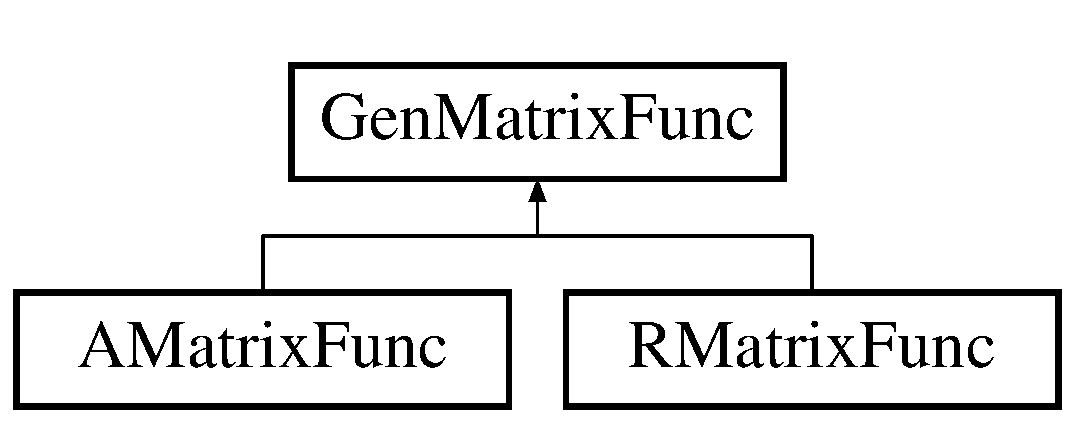
\includegraphics[height=2cm]{classGenMatrixFunc}
\end{center}
\end{figure}
\subsection*{Public Member Functions}
\begin{CompactItemize}
\item 
virtual void \bf{Clear\-Matrices} ()=0
\item 
virtual void \bf{Fill\-Matrices} (\bf{EPoint} $\ast$)=0
\item 
virtual void \bf{Invert\-Matrices} ()=0
\item 
virtual void \bf{Calculate\-TMatrix} (\bf{EPoint} $\ast$)=0
\item 
void \bf{Calculate\-Cross\-Section} (\bf{EPoint} $\ast$)
\item 
void \bf{New\-Temp\-TMatrix} (\bf{Temp\-TMatrix})
\item 
void \bf{Add\-To\-Temp\-TMatrix} (int, std::complex$<$ double $>$)
\item 
void \bf{Clear\-Temp\-TMatrices} ()
\item 
void \bf{Add\-TMatrix\-Element} (int, int, std::complex$<$ double $>$)
\item 
void \bf{Add\-ECTMatrix\-Element} (int, int, std::complex$<$ double $>$)
\item 
int \bf{Is\-Temp\-TMatrix} (double, int, int)
\item 
int \bf{Num\-Temp\-TMatrices} () const 
\item 
\bf{Temp\-TMatrix} $\ast$ \bf{Get\-Temp\-TMatrix} (int)
\item 
std::complex$<$ double $>$ \bf{Get\-TMatrix\-Element} (int, int) const 
\item 
std::complex$<$ double $>$ \bf{Get\-ECTMatrix\-Element} (int, int) const 
\item 
virtual \bf{CNuc} $\ast$ \bf{compound} () const =0
\end{CompactItemize}
\subsection*{Protected Attributes}
\begin{CompactItemize}
\item 
std::vector$<$ std::vector$<$ std::complex$<$ double $>$ $>$ $>$ \bf{tmatrix\_\-}\label{classGenMatrixFunc_4323d54cb869029b46d7e8dcc362f741}

\begin{CompactList}\small\item\em Vector of internal T-matrix elements accessable to child class. \item\end{CompactList}\item 
std::vector$<$ std::vector$<$ std::complex$<$ double $>$ $>$ $>$ \bf{ec\_\-tmatrix\_\-}\label{classGenMatrixFunc_92c63e76791a989432ee00865ff5e564}

\begin{CompactList}\small\item\em Vector of external T-matrix elements accessable to child class. \item\end{CompactList}\end{CompactItemize}


\subsection{Detailed Description}
A generalized function class to calculate cross sections. 

The \doxyref{Gen\-Matrix\-Func}{p.}{classGenMatrixFunc} function class is the general form of the function used to calculate cross section from R-Matrix parameters. It is the parent class of \doxyref{AMatrix\-Func}{p.}{classAMatrixFunc} and \doxyref{RMatrix\-Func}{p.}{classRMatrixFunc}. 



\subsection{Member Function Documentation}
\index{GenMatrixFunc@{Gen\-Matrix\-Func}!AddECTMatrixElement@{AddECTMatrixElement}}
\index{AddECTMatrixElement@{AddECTMatrixElement}!GenMatrixFunc@{Gen\-Matrix\-Func}}
\subsubsection{\setlength{\rightskip}{0pt plus 5cm}void Gen\-Matrix\-Func::Add\-ECTMatrix\-Element (int {\em k\-Group\-Num}, int {\em m\-Group\-Num}, std::complex$<$ double $>$ {\em t\-Matrix\-Element})}\label{classGenMatrixFunc_b6230f89dcc3dc68fb0c1f58a00ee530}


Adds an external T-Matrix element to the vector of external T-matrix elements corresponding to a specified external reaction pathway. \index{GenMatrixFunc@{Gen\-Matrix\-Func}!AddTMatrixElement@{AddTMatrixElement}}
\index{AddTMatrixElement@{AddTMatrixElement}!GenMatrixFunc@{Gen\-Matrix\-Func}}
\subsubsection{\setlength{\rightskip}{0pt plus 5cm}void Gen\-Matrix\-Func::Add\-TMatrix\-Element (int {\em k\-Group\-Num}, int {\em m\-Group\-Num}, std::complex$<$ double $>$ {\em t\-Matrix\-Element})}\label{classGenMatrixFunc_018c90b4443ef132ee0f1c83b83032b3}


Adds an internal T-Matrix element to the vector of internal T-matrix elements corresponding to a specified internal reaction pathway. \index{GenMatrixFunc@{Gen\-Matrix\-Func}!AddToTempTMatrix@{AddToTempTMatrix}}
\index{AddToTempTMatrix@{AddToTempTMatrix}!GenMatrixFunc@{Gen\-Matrix\-Func}}
\subsubsection{\setlength{\rightskip}{0pt plus 5cm}void Gen\-Matrix\-Func::Add\-To\-Temp\-TMatrix (int {\em temp\-TMatrix\-Num}, std::complex$<$ double $>$ {\em temp\-Value})}\label{classGenMatrixFunc_4a0a1f8bf9270df1d719b16b7bdb0871}


Adds a value to the temporary T-Matrix element specified by its position in the \doxyref{Temp\-TMatrix}{p.}{structTempTMatrix} vector. \index{GenMatrixFunc@{Gen\-Matrix\-Func}!CalculateCrossSection@{CalculateCrossSection}}
\index{CalculateCrossSection@{CalculateCrossSection}!GenMatrixFunc@{Gen\-Matrix\-Func}}
\subsubsection{\setlength{\rightskip}{0pt plus 5cm}void Gen\-Matrix\-Func::Calculate\-Cross\-Section (\bf{EPoint} $\ast$ {\em point})}\label{classGenMatrixFunc_f5057fff589739f1a8167725b15be1e1}


The child classes \doxyref{AMatrix\-Func}{p.}{classAMatrixFunc} or \doxyref{RMatrix\-Func}{p.}{classRMatrixFunc} contain functions to calculate the T-Matrix from the fitted R-Matrix parameters. This function then calculates the cross section from the T-Matrix elements. \index{GenMatrixFunc@{Gen\-Matrix\-Func}!CalculateTMatrix@{CalculateTMatrix}}
\index{CalculateTMatrix@{CalculateTMatrix}!GenMatrixFunc@{Gen\-Matrix\-Func}}
\subsubsection{\setlength{\rightskip}{0pt plus 5cm}virtual void Gen\-Matrix\-Func::Calculate\-TMatrix (\bf{EPoint} $\ast$)\hspace{0.3cm}{\tt  [pure virtual]}}\label{classGenMatrixFunc_f89bf73a0a2f230c2187947520c1f360}


This virtual function in instantiated in the child class. 

Implemented in \bf{AMatrix\-Func} \doxyref{p.}{classAMatrixFunc_6a4b63537f9c4716afc2cf03874ae2f3}, and \bf{RMatrix\-Func} \doxyref{p.}{classRMatrixFunc_62be4a71a76ecdbb75277b62cf30f0e8}.\index{GenMatrixFunc@{Gen\-Matrix\-Func}!ClearMatrices@{ClearMatrices}}
\index{ClearMatrices@{ClearMatrices}!GenMatrixFunc@{Gen\-Matrix\-Func}}
\subsubsection{\setlength{\rightskip}{0pt plus 5cm}virtual void Gen\-Matrix\-Func::Clear\-Matrices ()\hspace{0.3cm}{\tt  [pure virtual]}}\label{classGenMatrixFunc_41a9098087eac97b9c7de7aee82fa3d8}


This virtual function in instantiated in the child class. 

Implemented in \bf{AMatrix\-Func} \doxyref{p.}{classAMatrixFunc_9fa5a3ed65bf42990f74fe4cb482eb02}, and \bf{RMatrix\-Func} \doxyref{p.}{classRMatrixFunc_ef604251f6135d99ccf051e623d76ad7}.\index{GenMatrixFunc@{Gen\-Matrix\-Func}!ClearTempTMatrices@{ClearTempTMatrices}}
\index{ClearTempTMatrices@{ClearTempTMatrices}!GenMatrixFunc@{Gen\-Matrix\-Func}}
\subsubsection{\setlength{\rightskip}{0pt plus 5cm}void Gen\-Matrix\-Func::Clear\-Temp\-TMatrices ()}\label{classGenMatrixFunc_5bd96db58053c872624d03547c1a3d35}


Clears the temporary T-Matrices. \index{GenMatrixFunc@{Gen\-Matrix\-Func}!compound@{compound}}
\index{compound@{compound}!GenMatrixFunc@{Gen\-Matrix\-Func}}
\subsubsection{\setlength{\rightskip}{0pt plus 5cm}virtual \bf{CNuc}$\ast$ Gen\-Matrix\-Func::compound () const\hspace{0.3cm}{\tt  [pure virtual]}}\label{classGenMatrixFunc_12603673326e93fb80d8db05fad085de}


This virtual function in instantiated in the child class. 

Implemented in \bf{AMatrix\-Func} \doxyref{p.}{classAMatrixFunc_edf46d126dcf0748e0325bf39cbedde9}, and \bf{RMatrix\-Func} \doxyref{p.}{classRMatrixFunc_9cfee7ffe97466ba19e1e5014567713a}.\index{GenMatrixFunc@{Gen\-Matrix\-Func}!FillMatrices@{FillMatrices}}
\index{FillMatrices@{FillMatrices}!GenMatrixFunc@{Gen\-Matrix\-Func}}
\subsubsection{\setlength{\rightskip}{0pt plus 5cm}virtual void Gen\-Matrix\-Func::Fill\-Matrices (\bf{EPoint} $\ast$)\hspace{0.3cm}{\tt  [pure virtual]}}\label{classGenMatrixFunc_0ce6fcce1afbd13bfdb753fcdfbe196c}


This virtual function in instantiated in the child class. 

Implemented in \bf{AMatrix\-Func} \doxyref{p.}{classAMatrixFunc_953efa806622175437e1207c8fcda61c}, and \bf{RMatrix\-Func} \doxyref{p.}{classRMatrixFunc_7ad8de01bb08e66e2576bbb0271ff65b}.\index{GenMatrixFunc@{Gen\-Matrix\-Func}!GetECTMatrixElement@{GetECTMatrixElement}}
\index{GetECTMatrixElement@{GetECTMatrixElement}!GenMatrixFunc@{Gen\-Matrix\-Func}}
\subsubsection{\setlength{\rightskip}{0pt plus 5cm}std::complex$<$ double $>$ Gen\-Matrix\-Func::Get\-ECTMatrix\-Element (int {\em k\-Group\-Num}, int {\em ec\-MGroup\-Num}) const}\label{classGenMatrixFunc_3f0ce191518c353f7630195ab14e53ab}


Returns the value of the external T-Matrix element specified by an external reaction pathway. \index{GenMatrixFunc@{Gen\-Matrix\-Func}!GetTempTMatrix@{GetTempTMatrix}}
\index{GetTempTMatrix@{GetTempTMatrix}!GenMatrixFunc@{Gen\-Matrix\-Func}}
\subsubsection{\setlength{\rightskip}{0pt plus 5cm}\bf{Temp\-TMatrix} $\ast$ Gen\-Matrix\-Func::Get\-Temp\-TMatrix (int {\em temp\-TMatrix\-Num})}\label{classGenMatrixFunc_f944a69b7436a9c5a02954be6e98724b}


Returns a pointer to the temporary T-Matrix element specified by a position in the \doxyref{Temp\-TMatrix}{p.}{structTempTMatrix} vector. \index{GenMatrixFunc@{Gen\-Matrix\-Func}!GetTMatrixElement@{GetTMatrixElement}}
\index{GetTMatrixElement@{GetTMatrixElement}!GenMatrixFunc@{Gen\-Matrix\-Func}}
\subsubsection{\setlength{\rightskip}{0pt plus 5cm}std::complex$<$ double $>$ Gen\-Matrix\-Func::Get\-TMatrix\-Element (int {\em k\-Group\-Num}, int {\em m\-Group\-Num}) const}\label{classGenMatrixFunc_60c540bfff705cb7af6f4a3f38b22dec}


Returns the value of the internal T-Matrix element specified by an internal reaction pathway. \index{GenMatrixFunc@{Gen\-Matrix\-Func}!InvertMatrices@{InvertMatrices}}
\index{InvertMatrices@{InvertMatrices}!GenMatrixFunc@{Gen\-Matrix\-Func}}
\subsubsection{\setlength{\rightskip}{0pt plus 5cm}virtual void Gen\-Matrix\-Func::Invert\-Matrices ()\hspace{0.3cm}{\tt  [pure virtual]}}\label{classGenMatrixFunc_2dbfafa4c608ad5c1b27db7684f8f839}


This virtual function in instantiated in the child class. 

Implemented in \bf{AMatrix\-Func} \doxyref{p.}{classAMatrixFunc_cf45883ba4979a32596214d356b48766}, and \bf{RMatrix\-Func} \doxyref{p.}{classRMatrixFunc_b67c0ad184bf6e38343b5c24e64a9b43}.\index{GenMatrixFunc@{Gen\-Matrix\-Func}!IsTempTMatrix@{IsTempTMatrix}}
\index{IsTempTMatrix@{IsTempTMatrix}!GenMatrixFunc@{Gen\-Matrix\-Func}}
\subsubsection{\setlength{\rightskip}{0pt plus 5cm}int Gen\-Matrix\-Func::Is\-Temp\-TMatrix (double {\em j\-Value}, int {\em l\-Value}, int {\em l\-Prime\-Value})}\label{classGenMatrixFunc_91ad5da3beeaaa87f8359a5ce2af12c3}


Tests if a temporary T-Matrix element already exists for a given $ J,l,l' $ combination. If the element exists, returns the position in the \doxyref{Temp\-TMatrix}{p.}{structTempTMatrix} vector, otherwise returns 0. \index{GenMatrixFunc@{Gen\-Matrix\-Func}!NewTempTMatrix@{NewTempTMatrix}}
\index{NewTempTMatrix@{NewTempTMatrix}!GenMatrixFunc@{Gen\-Matrix\-Func}}
\subsubsection{\setlength{\rightskip}{0pt plus 5cm}void Gen\-Matrix\-Func::New\-Temp\-TMatrix (\bf{Temp\-TMatrix} {\em temp\-TMatrix})}\label{classGenMatrixFunc_623817601830fa134f89d0ee22fead84}


Creates a new temporary T-Matrix element. \index{GenMatrixFunc@{Gen\-Matrix\-Func}!NumTempTMatrices@{NumTempTMatrices}}
\index{NumTempTMatrices@{NumTempTMatrices}!GenMatrixFunc@{Gen\-Matrix\-Func}}
\subsubsection{\setlength{\rightskip}{0pt plus 5cm}int Gen\-Matrix\-Func::Num\-Temp\-TMatrices () const}\label{classGenMatrixFunc_d28bbc9e9c8fb7571ec8305fe0b9ffe4}


Returns the number of temporary T-Matrix elements in the \doxyref{Temp\-TMatrix}{p.}{structTempTMatrix} vector. 

The documentation for this class was generated from the following files:\begin{CompactItemize}
\item 
azure\_\-v2/include/Gen\-Matrix\-Func.h\item 
azure\_\-v2/src/Gen\-Matrix\-Func.cpp\end{CompactItemize}

\section{Interference Class Reference}
\label{classInterference}\index{Interference@{Interference}}
An AZURE $ l_1,l_2,l_1',l_2',J_1,J_2 $ combination.  


{\tt \#include $<$Interference.h$>$}

\subsection*{Public Member Functions}
\begin{CompactItemize}
\item 
\bf{Interference} (int, int, double, std::string)
\item 
std::string \bf{Get\-Interference\-Type} () const 
\item 
int \bf{Get\-M1} () const 
\item 
int \bf{Get\-M2} () const 
\item 
double \bf{Get\-Z1Z2} () const 
\end{CompactItemize}


\subsection{Detailed Description}
An AZURE $ l_1,l_2,l_1',l_2',J_1,J_2 $ combination. 

In the differential cross section formula of R-Matrix, nested inside the $ s,s',L $ sum is a sum over $ l_1,l_2,l_1',l_2',J_1,J_2 $. In the language of AZURE, these are equivalent to combinations of two reaction pathways. If the pathways are the same, the term represents the actual contribution from the pathway to the cross section. If they are different, the term represents the interference between the two. 



\subsection{Constructor \& Destructor Documentation}
\index{Interference@{Interference}!Interference@{Interference}}
\index{Interference@{Interference}!Interference@{Interference}}
\subsubsection{\setlength{\rightskip}{0pt plus 5cm}Interference::Interference (int {\em m\-Group\-Num1}, int {\em m\-Group\-Num2}, double {\em z1z2Coeff}, std::string {\em interference\-Type})}\label{classInterference_58ea9ce8846dfc0b6061ac4c4871ad36}


The pathways combination is created specifically using references to two positions in the Croup and \doxyref{ECMGroup}{p.}{classECMGroup} vectors under the corresponding \doxyref{KGroup}{p.}{classKGroup} object. Additionally, the $ Z_1 Z_2 $ coefficients are passed along with the interference type. The interference type is either RR, ER, RE,or EE, indicating which vector, the \doxyref{MGroup}{p.}{classMGroup} or \doxyref{ECMGroup}{p.}{classECMGroup}, the stored indices refer to. 

\subsection{Member Function Documentation}
\index{Interference@{Interference}!GetInterferenceType@{GetInterferenceType}}
\index{GetInterferenceType@{GetInterferenceType}!Interference@{Interference}}
\subsubsection{\setlength{\rightskip}{0pt plus 5cm}std::string Interference::Get\-Interference\-Type () const}\label{classInterference_d749cdab1478c11dfea99b9c244f7dd0}


Returns the interference type. \index{Interference@{Interference}!GetM1@{GetM1}}
\index{GetM1@{GetM1}!Interference@{Interference}}
\subsubsection{\setlength{\rightskip}{0pt plus 5cm}int Interference::Get\-M1 () const}\label{classInterference_5f8a468df77bebe5bfd40740ac73c088}


Returns the position in the \doxyref{MGroup}{p.}{classMGroup} or \doxyref{ECMGroup}{p.}{classECMGroup} vector of the first pathway. \index{Interference@{Interference}!GetM2@{GetM2}}
\index{GetM2@{GetM2}!Interference@{Interference}}
\subsubsection{\setlength{\rightskip}{0pt plus 5cm}int Interference::Get\-M2 () const}\label{classInterference_7ccbee61fe1b04da55b4a27aabfda8f7}


Returns the position in the \doxyref{MGroup}{p.}{classMGroup} or \doxyref{ECMGroup}{p.}{classECMGroup} vector of the second pathway. \index{Interference@{Interference}!GetZ1Z2@{GetZ1Z2}}
\index{GetZ1Z2@{GetZ1Z2}!Interference@{Interference}}
\subsubsection{\setlength{\rightskip}{0pt plus 5cm}double Interference::Get\-Z1Z2 () const}\label{classInterference_d6d173c6b5f7129ee747d69daf863c1f}


Returns the corresponding $ Z_1 Z_2 $ coefficient. 

The documentation for this class was generated from the following files:\begin{CompactItemize}
\item 
azure\_\-v2/include/Interference.h\item 
azure\_\-v2/src/Interference.cpp\end{CompactItemize}

\section{JGroup Class Reference}
\label{classJGroup}\index{JGroup@{JGroup}}
An AZURE $ J^\pi $ group.  


{\tt \#include $<$JGroup.h$>$}

\subsection*{Public Member Functions}
\begin{CompactItemize}
\item 
\bf{JGroup} (Nuc\-Line)
\item 
\bf{JGroup} (double, int)
\item 
bool \bf{Is\-In\-RMatrix} () const 
\item 
int \bf{Is\-Level} (\bf{ALevel})
\item 
int \bf{Get\-Pi} () const 
\item 
int \bf{Num\-Levels} () const 
\item 
int \bf{Num\-Channels} ()
\item 
int \bf{Is\-Channel} (\bf{AChannel})
\item 
double \bf{Get\-J} () const 
\item 
void \bf{Add\-Level} (\bf{ALevel})
\item 
void \bf{Add\-Channel} (\bf{AChannel})
\item 
\bf{AChannel} $\ast$ \bf{Get\-Channel} (int)
\item 
\bf{ALevel} $\ast$ \bf{Get\-Level} (int)
\end{CompactItemize}


\subsection{Detailed Description}
An AZURE $ J^\pi $ group. 

In R-Matrix theory, levels are grouped according to their $ J^\pi $ values. There is one R-/A-Matrix, and thus one T-Matrix, for each $ J^\pi $ group. A \doxyref{JGroup}{p.}{classJGroup} object holds vectors of \doxyref{ALevel}{p.}{classALevel} and \doxyref{AChannel}{p.}{classAChannel} objects. 



\subsection{Constructor \& Destructor Documentation}
\index{JGroup@{JGroup}!JGroup@{JGroup}}
\index{JGroup@{JGroup}!JGroup@{JGroup}}
\subsubsection{\setlength{\rightskip}{0pt plus 5cm}JGroup::JGroup (Nuc\-Line {\em nuc\-Line})}\label{classJGroup_173b8e04a5204518395c4e7d86831cd0}


This constructor is used when a $ J^\pi $ group is created from an entry in the nuclear input file. \index{JGroup@{JGroup}!JGroup@{JGroup}}
\index{JGroup@{JGroup}!JGroup@{JGroup}}
\subsubsection{\setlength{\rightskip}{0pt plus 5cm}JGroup::JGroup (double {\em j}, int {\em pi})}\label{classJGroup_1d23d2e2222a29f4331d7aa8f848a22e}


This constructor is used when a $ J^\pi $ group is created from specified values of spin and parity. 

\subsection{Member Function Documentation}
\index{JGroup@{JGroup}!AddChannel@{AddChannel}}
\index{AddChannel@{AddChannel}!JGroup@{JGroup}}
\subsubsection{\setlength{\rightskip}{0pt plus 5cm}void JGroup::Add\-Channel (\bf{AChannel} {\em channel})}\label{classJGroup_8ca9ab8c954a41a099cb2c3386860323}


Adds a new channel to the vector of \doxyref{AChannel}{p.}{classAChannel} objects. \index{JGroup@{JGroup}!AddLevel@{AddLevel}}
\index{AddLevel@{AddLevel}!JGroup@{JGroup}}
\subsubsection{\setlength{\rightskip}{0pt plus 5cm}void JGroup::Add\-Level (\bf{ALevel} {\em level})}\label{classJGroup_5ffe8fb456f5e459f976cd6c7ca554d0}


Adds a new level to the vector of \doxyref{ALevel}{p.}{classALevel} objects. \index{JGroup@{JGroup}!GetChannel@{GetChannel}}
\index{GetChannel@{GetChannel}!JGroup@{JGroup}}
\subsubsection{\setlength{\rightskip}{0pt plus 5cm}\bf{AChannel} $\ast$ JGroup::Get\-Channel (int {\em channel\-Num})}\label{classJGroup_53f91b0a2820cf092c911fe5bd0e0a9c}


Returns a pointer to a specified channel in the \doxyref{AChannel}{p.}{classAChannel} vector. \index{JGroup@{JGroup}!GetJ@{GetJ}}
\index{GetJ@{GetJ}!JGroup@{JGroup}}
\subsubsection{\setlength{\rightskip}{0pt plus 5cm}double JGroup::Get\-J () const}\label{classJGroup_579020bf091d4c6809a4c1813507d05b}


Returns the spin value of the $ J^\pi $ group. \index{JGroup@{JGroup}!GetLevel@{GetLevel}}
\index{GetLevel@{GetLevel}!JGroup@{JGroup}}
\subsubsection{\setlength{\rightskip}{0pt plus 5cm}\bf{ALevel} $\ast$ JGroup::Get\-Level (int {\em level\-Num})}\label{classJGroup_5374a525ba80cc12ed6c319e69c0f782}


Returns a pointer to a specified level in the \doxyref{ALevel}{p.}{classALevel} vector. \index{JGroup@{JGroup}!GetPi@{GetPi}}
\index{GetPi@{GetPi}!JGroup@{JGroup}}
\subsubsection{\setlength{\rightskip}{0pt plus 5cm}int JGroup::Get\-Pi () const}\label{classJGroup_1e0789327811d2d337a536561393a42d}


Returns the parity of the the $ J^\pi $ group as $ \pm1 $. \index{JGroup@{JGroup}!IsChannel@{IsChannel}}
\index{IsChannel@{IsChannel}!JGroup@{JGroup}}
\subsubsection{\setlength{\rightskip}{0pt plus 5cm}int JGroup::Is\-Channel (\bf{AChannel} {\em channel})}\label{classJGroup_5c421ccd20d1db4c83c3bf67910be004}


This function tests if a given channel already exists in the vector of \doxyref{AChannel}{p.}{classAChannel} objects. If the channel exists the position of the channel in the vector is returned, otherwise the function returns 0. \index{JGroup@{JGroup}!IsInRMatrix@{IsInRMatrix}}
\index{IsInRMatrix@{IsInRMatrix}!JGroup@{JGroup}}
\subsubsection{\setlength{\rightskip}{0pt plus 5cm}bool JGroup::Is\-In\-RMatrix () const}\label{classJGroup_70d5c23420a1a5ba74e3de62c5e9f749}


Returns true if the $ J^\pi $ group is to be included in the A-/R-Matrix calculation, otherwise returns false. A $ J^\pi $ group may specify only a bound state for external capture, but may not correspond to an R-Matrix state (i.e. subthreshold state). \index{JGroup@{JGroup}!IsLevel@{IsLevel}}
\index{IsLevel@{IsLevel}!JGroup@{JGroup}}
\subsubsection{\setlength{\rightskip}{0pt plus 5cm}int JGroup::Is\-Level (\bf{ALevel} {\em level})}\label{classJGroup_02ec8f85160d0c9af4557c2575e6b68e}


This function tests if a given level already exists in the vector of \doxyref{ALevel}{p.}{classALevel} objects. If the level exists the position of the level in the vector is returned, otherwise the function returns 0. \index{JGroup@{JGroup}!NumChannels@{NumChannels}}
\index{NumChannels@{NumChannels}!JGroup@{JGroup}}
\subsubsection{\setlength{\rightskip}{0pt plus 5cm}int JGroup::Num\-Channels ()}\label{classJGroup_b0ac472d15f38258b05e4a4e559e8900}


Returns the number of channels in the \doxyref{AChannel}{p.}{classAChannel} vector. \index{JGroup@{JGroup}!NumLevels@{NumLevels}}
\index{NumLevels@{NumLevels}!JGroup@{JGroup}}
\subsubsection{\setlength{\rightskip}{0pt plus 5cm}int JGroup::Num\-Levels () const}\label{classJGroup_0ba1e7b32633b9170a6c7e9be7e18a06}


Returns the number of levels in the \doxyref{ALevel}{p.}{classALevel} vector. 

The documentation for this class was generated from the following files:\begin{CompactItemize}
\item 
azure\_\-v2/include/JGroup.h\item 
azure\_\-v2/src/JGroup.cpp\end{CompactItemize}

\section{KGroup Class Reference}
\label{classKGroup}\index{KGroup@{KGroup}}
An AZURE $ s,s' $ group.  


{\tt \#include $<$KGroup.h$>$}

\subsection*{Public Member Functions}
\begin{CompactItemize}
\item 
\bf{KGroup} (double, double)
\item 
int \bf{Num\-MGroups} () const 
\item 
int \bf{Num\-ECMGroups} () const 
\item 
int \bf{Is\-MGroup} (\bf{MGroup})
\item 
double \bf{Get\-S} () const 
\item 
double \bf{Get\-Sp} () const 
\item 
void \bf{Add\-MGroup} (\bf{MGroup})
\item 
void \bf{Add\-ECMGroup} (\bf{ECMGroup})
\item 
\bf{MGroup} $\ast$ \bf{Get\-MGroup} (int)
\item 
\bf{ECMGroup} $\ast$ \bf{Get\-ECMGroup} (int)
\end{CompactItemize}


\subsection{Detailed Description}
An AZURE $ s,s' $ group. 

In R-Matrix formalism, the equations required to calculate the cross section usually nested inside sums over entrance and exit channel spins. For this reason AZURE groups reaction pathways according to their entrance and exit channel spins. Each \doxyref{KGroup}{p.}{classKGroup} object is a container for vectors of \doxyref{MGroup}{p.}{classMGroup} and \doxyref{ECMGroup}{p.}{classECMGroup} objects. 



\subsection{Constructor \& Destructor Documentation}
\index{KGroup@{KGroup}!KGroup@{KGroup}}
\index{KGroup@{KGroup}!KGroup@{KGroup}}
\subsubsection{\setlength{\rightskip}{0pt plus 5cm}KGroup::KGroup (double {\em s}, double {\em s\-Prime})}\label{classKGroup_cc31d5f411bb708013511435ada3a56d}


The \doxyref{KGroup}{p.}{classKGroup} is created from a specific combination of entrance and exit channel spin values. 

\subsection{Member Function Documentation}
\index{KGroup@{KGroup}!AddECMGroup@{AddECMGroup}}
\index{AddECMGroup@{AddECMGroup}!KGroup@{KGroup}}
\subsubsection{\setlength{\rightskip}{0pt plus 5cm}void KGroup::Add\-ECMGroup (\bf{ECMGroup} {\em ec\-MGroup})}\label{classKGroup_e8aa02df7e42b68fed05118f887f1997}


Adds a new external reaction pathway to the \doxyref{ECMGroup}{p.}{classECMGroup} vector. \index{KGroup@{KGroup}!AddMGroup@{AddMGroup}}
\index{AddMGroup@{AddMGroup}!KGroup@{KGroup}}
\subsubsection{\setlength{\rightskip}{0pt plus 5cm}void KGroup::Add\-MGroup (\bf{MGroup} {\em m\-Group})}\label{classKGroup_c6291fd7bba6f207f840efdc0788ce1a}


Adds a new internal reaction pathway to the \doxyref{MGroup}{p.}{classMGroup} vector. \index{KGroup@{KGroup}!GetECMGroup@{GetECMGroup}}
\index{GetECMGroup@{GetECMGroup}!KGroup@{KGroup}}
\subsubsection{\setlength{\rightskip}{0pt plus 5cm}\bf{ECMGroup} $\ast$ KGroup::Get\-ECMGroup (int {\em ec\-MGroup\-Num})}\label{classKGroup_0e7742826efc97a3e130bb468f5529be}


Returns a pointer to the external reaction pathway specified by a position in the \doxyref{ECMGroup}{p.}{classECMGroup} vector. \index{KGroup@{KGroup}!GetMGroup@{GetMGroup}}
\index{GetMGroup@{GetMGroup}!KGroup@{KGroup}}
\subsubsection{\setlength{\rightskip}{0pt plus 5cm}\bf{MGroup} $\ast$ KGroup::Get\-MGroup (int {\em m\-Group\-Num})}\label{classKGroup_43ae8136504381fba272570e40da4446}


Returns a pointer to the internal reaction pathway specified by a position in the \doxyref{MGroup}{p.}{classMGroup} vector. \index{KGroup@{KGroup}!GetS@{GetS}}
\index{GetS@{GetS}!KGroup@{KGroup}}
\subsubsection{\setlength{\rightskip}{0pt plus 5cm}double KGroup::Get\-S () const}\label{classKGroup_3d3145a1926d059370f4b89c89034bba}


Returns the value of the entrance channel spin. \index{KGroup@{KGroup}!GetSp@{GetSp}}
\index{GetSp@{GetSp}!KGroup@{KGroup}}
\subsubsection{\setlength{\rightskip}{0pt plus 5cm}double KGroup::Get\-Sp () const}\label{classKGroup_fb93cc01d04262199c5bbb429ad00e77}


Returns the value of the exit channel spin. \index{KGroup@{KGroup}!IsMGroup@{IsMGroup}}
\index{IsMGroup@{IsMGroup}!KGroup@{KGroup}}
\subsubsection{\setlength{\rightskip}{0pt plus 5cm}int KGroup::Is\-MGroup (\bf{MGroup} {\em m\-Group})}\label{classKGroup_a11309fd33b3afbf7b965298d81a0dbd}


Tests a specific internal reaction pathway to see if it already exists in the \doxyref{MGroup}{p.}{classMGroup} vector. If the pathway exists, its position in the vector is returned. Otherwise, the function returns 0. \index{KGroup@{KGroup}!NumECMGroups@{NumECMGroups}}
\index{NumECMGroups@{NumECMGroups}!KGroup@{KGroup}}
\subsubsection{\setlength{\rightskip}{0pt plus 5cm}int KGroup::Num\-ECMGroups () const}\label{classKGroup_ec7e8375f393a4acd4a7abc645fba46f}


Returns the number of external reaction pathways in the \doxyref{ECMGroup}{p.}{classECMGroup} vector; \index{KGroup@{KGroup}!NumMGroups@{NumMGroups}}
\index{NumMGroups@{NumMGroups}!KGroup@{KGroup}}
\subsubsection{\setlength{\rightskip}{0pt plus 5cm}int KGroup::Num\-MGroups () const}\label{classKGroup_4c4ea1e1611bbd222e7c757baf42c2a6}


Returns the number of internal reaction pathways in the \doxyref{MGroup}{p.}{classMGroup} vector. 

The documentation for this class was generated from the following files:\begin{CompactItemize}
\item 
azure\_\-v2/include/KGroup.h\item 
azure\_\-v2/src/KGroup.cpp\end{CompactItemize}

\section{KLGroup Class Reference}
\label{classKLGroup}\index{KLGroup@{KLGroup}}
An AZURE $ s,s',L $ group.  


{\tt \#include $<$KLGroup.h$>$}

\subsection*{Public Member Functions}
\begin{CompactItemize}
\item 
\bf{KLGroup} (int, int)
\item 
int \bf{Get\-K} () const 
\item 
int \bf{Get\-LOrder} () const 
\item 
int \bf{Num\-Interferences} () const 
\item 
int \bf{Is\-Interference} (\bf{Interference})
\item 
void \bf{Add\-Interference} (\bf{Interference})
\item 
\bf{Interference} $\ast$ \bf{Get\-Interference} (int)
\end{CompactItemize}


\subsection{Detailed Description}
An AZURE $ s,s',L $ group. 

Differential cross sections in R-Matrix theory contains terms nested inside a sum over entrance and exit spins as well as Legendre polynomial orders, $ L $. In AZURE, an $ s,s' $ combination is given by a \doxyref{KGroup}{p.}{classKGroup} object. It is therefore convenient to group \doxyref{KGroup}{p.}{classKGroup} objects with a specified polynomial orders for the calculation of differenial cross sections. The \doxyref{KLGroup}{p.}{classKLGroup} object serves as a container class for a vector of \doxyref{Interference}{p.}{classInterference} objects. 



\subsection{Constructor \& Destructor Documentation}
\index{KLGroup@{KLGroup}!KLGroup@{KLGroup}}
\index{KLGroup@{KLGroup}!KLGroup@{KLGroup}}
\subsubsection{\setlength{\rightskip}{0pt plus 5cm}KLGroup::KLGroup (int {\em k\-Group\-Num}, int {\em l\-Order})}\label{classKLGroup_f88c94714230e6c974f77b06c76fff10}


The object is created with reference to a specfic \doxyref{KGroup}{p.}{classKGroup} number as well as Legendre polynomial order. 

\subsection{Member Function Documentation}
\index{KLGroup@{KLGroup}!AddInterference@{AddInterference}}
\index{AddInterference@{AddInterference}!KLGroup@{KLGroup}}
\subsubsection{\setlength{\rightskip}{0pt plus 5cm}void KLGroup::Add\-Interference (\bf{Interference} {\em interference})}\label{classKLGroup_13c2a937a069f80d981a544927c1b9b2}


Adds an interference combination to the \doxyref{Interference}{p.}{classInterference} vector. \index{KLGroup@{KLGroup}!GetInterference@{GetInterference}}
\index{GetInterference@{GetInterference}!KLGroup@{KLGroup}}
\subsubsection{\setlength{\rightskip}{0pt plus 5cm}\bf{Interference} $\ast$ KLGroup::Get\-Interference (int {\em interference\-Num})}\label{classKLGroup_80eb6ad5f1496c1a5a4491cbf0b985c7}


Returns a pointer to an interference combination specified by a position in the \doxyref{Interference}{p.}{classInterference} vector. \index{KLGroup@{KLGroup}!GetK@{GetK}}
\index{GetK@{GetK}!KLGroup@{KLGroup}}
\subsubsection{\setlength{\rightskip}{0pt plus 5cm}int KLGroup::Get\-K () const}\label{classKLGroup_6fd7904e825b6ca8e1c5638c35d59746}


Returns the position of the $ s,s' $ combination in the \doxyref{KGroup}{p.}{classKGroup} vector. \index{KLGroup@{KLGroup}!GetLOrder@{GetLOrder}}
\index{GetLOrder@{GetLOrder}!KLGroup@{KLGroup}}
\subsubsection{\setlength{\rightskip}{0pt plus 5cm}int KLGroup::Get\-LOrder () const}\label{classKLGroup_74f4425bedaf101a0dd8b68dbfe88008}


Returns the Legendre polynomial order. \index{KLGroup@{KLGroup}!IsInterference@{IsInterference}}
\index{IsInterference@{IsInterference}!KLGroup@{KLGroup}}
\subsubsection{\setlength{\rightskip}{0pt plus 5cm}int KLGroup::Is\-Interference (\bf{Interference} {\em interference})}\label{classKLGroup_34ae18648d5db467d6a1c9d691360b26}


Tests an interference combination to determine if it exists in the \doxyref{Interference}{p.}{classInterference} vector. If the combination exists, its position in the vector is returned. Otherwise, the function returns 0. \index{KLGroup@{KLGroup}!NumInterferences@{NumInterferences}}
\index{NumInterferences@{NumInterferences}!KLGroup@{KLGroup}}
\subsubsection{\setlength{\rightskip}{0pt plus 5cm}int KLGroup::Num\-Interferences () const}\label{classKLGroup_d4286b8f472fc83057e074287db7cb48}


Returns the number of interference combinations in the \doxyref{Interference}{p.}{classInterference} vector. 

The documentation for this class was generated from the following files:\begin{CompactItemize}
\item 
azure\_\-v2/include/KLGroup.h\item 
azure\_\-v2/src/KLGroup.cpp\end{CompactItemize}

\section{MGroup Class Reference}
\label{classMGroup}\index{MGroup@{MGroup}}
An AZURE internal reaction pathway.  


{\tt \#include $<$MGroup.h$>$}

\subsection*{Public Member Functions}
\begin{CompactItemize}
\item 
\bf{MGroup} (int, int, int)
\item 
int \bf{Get\-Ch\-Num} () const 
\item 
int \bf{Get\-Chp\-Num} () const 
\item 
int \bf{Get\-JNum} () const 
\item 
double \bf{Get\-Stat\-Spin\-Factor} () const 
\item 
void \bf{Set\-Stat\-Spin\-Factor} (double)
\end{CompactItemize}


\subsection{Detailed Description}
An AZURE internal reaction pathway. 

An \doxyref{MGroup}{p.}{classMGroup} in AZURE represents a given entrance and exit channel through a $ J^\pi $ group. These can be visualized as paths entering one row of the T-Matrix, and exiting through a column. 



\subsection{Constructor \& Destructor Documentation}
\index{MGroup@{MGroup}!MGroup@{MGroup}}
\index{MGroup@{MGroup}!MGroup@{MGroup}}
\subsubsection{\setlength{\rightskip}{0pt plus 5cm}MGroup::MGroup (int {\em j\-Group\-Num}, int {\em channel\-Num}, int {\em channel\-Prime\-Num})}\label{classMGroup_9fc3f4bb02717b01e3cc7f79f3640615}


This constructor is used to create an \doxyref{MGroup}{p.}{classMGroup} object with reference to positions in the \doxyref{JGroup}{p.}{classJGroup} and subsequent \doxyref{AChannel}{p.}{classAChannel} vectors. 

\subsection{Member Function Documentation}
\index{MGroup@{MGroup}!GetChNum@{GetChNum}}
\index{GetChNum@{GetChNum}!MGroup@{MGroup}}
\subsubsection{\setlength{\rightskip}{0pt plus 5cm}int MGroup::Get\-Ch\-Num () const}\label{classMGroup_d27fda3819de8fc41770a637604b67a4}


Returns the position of the entrance channel in the \doxyref{AChannel}{p.}{classAChannel} vector below the corresponding \doxyref{JGroup}{p.}{classJGroup} object. \index{MGroup@{MGroup}!GetChpNum@{GetChpNum}}
\index{GetChpNum@{GetChpNum}!MGroup@{MGroup}}
\subsubsection{\setlength{\rightskip}{0pt plus 5cm}int MGroup::Get\-Chp\-Num () const}\label{classMGroup_abc069de4e510ad77df8432d94ff397b}


Returns the position of the exit channel in the \doxyref{AChannel}{p.}{classAChannel} vector below the corresponding \doxyref{JGroup}{p.}{classJGroup} object. \index{MGroup@{MGroup}!GetJNum@{GetJNum}}
\index{GetJNum@{GetJNum}!MGroup@{MGroup}}
\subsubsection{\setlength{\rightskip}{0pt plus 5cm}int MGroup::Get\-JNum () const}\label{classMGroup_dcf3028b81b73ae5f41199f4ad1e350f}


Returns the position of the $ J^\pi $ group in the \doxyref{JGroup}{p.}{classJGroup} vector. \index{MGroup@{MGroup}!GetStatSpinFactor@{GetStatSpinFactor}}
\index{GetStatSpinFactor@{GetStatSpinFactor}!MGroup@{MGroup}}
\subsubsection{\setlength{\rightskip}{0pt plus 5cm}double MGroup::Get\-Stat\-Spin\-Factor () const}\label{classMGroup_e3dd037c11130b1b96ee80c603e26bbb}


Returns the statistical spin factor, $ g_J $, for the reaction pathway. \index{MGroup@{MGroup}!SetStatSpinFactor@{SetStatSpinFactor}}
\index{SetStatSpinFactor@{SetStatSpinFactor}!MGroup@{MGroup}}
\subsubsection{\setlength{\rightskip}{0pt plus 5cm}void MGroup::Set\-Stat\-Spin\-Factor (double {\em spin\-Factor})}\label{classMGroup_58b789a7b0b4975a71007827fa39e0bb}


Sets the statistical spin factor, $ g_J $, for the reaction pathway. 

The documentation for this class was generated from the following files:\begin{CompactItemize}
\item 
azure\_\-v2/include/MGroup.h\item 
azure\_\-v2/src/MGroup.cpp\end{CompactItemize}

\section{NFIntegral Class Reference}
\label{classNFIntegral}\index{NFIntegral@{NFIntegral}}
A function class to calculate the channel integrals in the denominator of the $ N_f^{1/2} $ term.  


{\tt \#include $<$NFIntegral.h$>$}

\subsection*{Public Member Functions}
\begin{CompactItemize}
\item 
\bf{NFIntegral} (\bf{PPair} $\ast$p\-Pair)
\item 
\bf{$\sim$NFIntegral} ()
\item 
double \bf{operator()} (int l\-Final, double level\-Energy) const 
\item 
\bf{Whit\-Func} $\ast$ \bf{whitfunction} () const 
\item 
double \bf{Chan\-Rad} () const 
\item 
double \bf{Total\-Sep\-E} () const 
\end{CompactItemize}


\subsection{Detailed Description}
A function class to calculate the channel integrals in the denominator of the $ N_f^{1/2} $ term. 

The \doxyref{NFIntegral}{p.}{classNFIntegral} class returns the channel integral given by $ \int_a^\infty \left[ \frac{W_c(kr)}{W_c{ka_c}} \right]^2 $. 



\subsection{Constructor \& Destructor Documentation}
\index{NFIntegral@{NFIntegral}!NFIntegral@{NFIntegral}}
\index{NFIntegral@{NFIntegral}!NFIntegral@{NFIntegral}}
\subsubsection{\setlength{\rightskip}{0pt plus 5cm}NFIntegral::NFIntegral (\bf{PPair} $\ast$ {\em p\-Pair})\hspace{0.3cm}{\tt  [inline]}}\label{classNFIntegral_0903eaf1f0b88701a265d7b4df04c649}


The \doxyref{NFIntegral}{p.}{classNFIntegral} object is created with reference to a \doxyref{PPair}{p.}{classPPair} object. A \doxyref{Whit\-Func}{p.}{classWhitFunc} object is also created. \index{NFIntegral@{NFIntegral}!~NFIntegral@{$\sim$NFIntegral}}
\index{~NFIntegral@{$\sim$NFIntegral}!NFIntegral@{NFIntegral}}
\subsubsection{\setlength{\rightskip}{0pt plus 5cm}NFIntegral::$\sim$NFIntegral ()\hspace{0.3cm}{\tt  [inline]}}\label{classNFIntegral_a27234f9f791514657077ba1275ecc67}


The \doxyref{Whit\-Func}{p.}{classWhitFunc} object is destroyed with the \doxyref{NFIntegral}{p.}{classNFIntegral} object. 

\subsection{Member Function Documentation}
\index{NFIntegral@{NFIntegral}!ChanRad@{ChanRad}}
\index{ChanRad@{ChanRad}!NFIntegral@{NFIntegral}}
\subsubsection{\setlength{\rightskip}{0pt plus 5cm}double NFIntegral::Chan\-Rad () const\hspace{0.3cm}{\tt  [inline]}}\label{classNFIntegral_380469e0861417012683d4968d3aabdb}


Returns the channel radius of the particle pair. \index{NFIntegral@{NFIntegral}!operator()@{operator()}}
\index{operator()@{operator()}!NFIntegral@{NFIntegral}}
\subsubsection{\setlength{\rightskip}{0pt plus 5cm}double NFIntegral::operator() (int {\em l\-Final}, double {\em level\-Energy}) const\hspace{0.3cm}{\tt  [inline]}}\label{classNFIntegral_b23bb498c13f4d1fd187722910253c48}


The parenthesis operator is defined so the instance can be callable as a function. The final channel orbital angular momentum and final state energy in the compound system are passed as dependent variables. \index{NFIntegral@{NFIntegral}!TotalSepE@{TotalSepE}}
\index{TotalSepE@{TotalSepE}!NFIntegral@{NFIntegral}}
\subsubsection{\setlength{\rightskip}{0pt plus 5cm}double NFIntegral::Total\-Sep\-E () const\hspace{0.3cm}{\tt  [inline]}}\label{classNFIntegral_c06458413d91d3e73f263b4b59a8c2aa}


Returns the total seperation energy of the particle pair. \index{NFIntegral@{NFIntegral}!whitfunction@{whitfunction}}
\index{whitfunction@{whitfunction}!NFIntegral@{NFIntegral}}
\subsubsection{\setlength{\rightskip}{0pt plus 5cm}\bf{Whit\-Func}$\ast$ NFIntegral::whitfunction () const\hspace{0.3cm}{\tt  [inline]}}\label{classNFIntegral_43f4f68138310de70338d3f5738768c3}


Returns a pointer to the \doxyref{Whit\-Func}{p.}{classWhitFunc} object. 

The documentation for this class was generated from the following file:\begin{CompactItemize}
\item 
azure\_\-v2/include/NFIntegral.h\end{CompactItemize}

\section{PPair Class Reference}
\label{classPPair}\index{PPair@{PPair}}
An AZURE Particle Pair.  


{\tt \#include $<$PPair.h$>$}

\subsection*{Public Member Functions}
\begin{CompactItemize}
\item 
\bf{PPair} (Nuc\-Line)
\item 
bool \bf{Is\-Entrance} () const 
\item 
bool \bf{Is\-ECEntrance} () const 
\item 
int \bf{Get\-Z} (int) const 
\item 
int \bf{Get\-Pi} (int) const 
\item 
int \bf{Get\-PType} () const 
\item 
int \bf{Num\-Decays} () const 
\item 
int \bf{Is\-Decay} (\bf{Decay})
\item 
int \bf{Is\-Decay} (int)
\item 
int \bf{Get\-Pair\-Key} () const 
\item 
int \bf{Num\-ECLevels} () const 
\item 
double \bf{Get\-M} (int) const 
\item 
double \bf{Get\-G} (int) const 
\item 
double \bf{Get\-J} (int) const 
\item 
double \bf{Get\-Ex\-E} () const 
\item 
double \bf{Get\-Sep\-E} () const 
\item 
double \bf{Get\-Ch\-Rad} () const 
\item 
double \bf{Get\-Red\-Mass} () const 
\item 
double \bf{Get\-I1I2Factor} () const 
\item 
void \bf{Add\-Decay} (\bf{Decay})
\item 
void \bf{Set\-Entrance} ()
\item 
void \bf{Set\-ECEntrance} ()
\item 
void \bf{Add\-ECLevel} (\bf{ECLevel})
\item 
\bf{Decay} $\ast$ \bf{Get\-Decay} (int)
\item 
\bf{ECLevel} $\ast$ \bf{Get\-ECLevel} (int)
\end{CompactItemize}


\subsection{Detailed Description}
An AZURE Particle Pair. 

In R-Matrix theory, the configuration space in the external region is decomposed into combinations of particle pairs, traditionally given by the symbol $ \alpha $. In AZURE, these particle pair are represented by a \doxyref{PPair}{p.}{classPPair} object. \doxyref{PPair}{p.}{classPPair} objects are containers for vectors of \doxyref{ECLevel}{p.}{classECLevel} and \doxyref{Decay}{p.}{classDecay} objects. 



\subsection{Constructor \& Destructor Documentation}
\index{PPair@{PPair}!PPair@{PPair}}
\index{PPair@{PPair}!PPair@{PPair}}
\subsubsection{\setlength{\rightskip}{0pt plus 5cm}PPair::PPair (Nuc\-Line {\em nuc\-Line})}\label{classPPair_c205bd01785825fe507d2e58acaac7e6}


A particle pair object is created from and entry in the nuclear input file. 

\subsection{Member Function Documentation}
\index{PPair@{PPair}!AddDecay@{AddDecay}}
\index{AddDecay@{AddDecay}!PPair@{PPair}}
\subsubsection{\setlength{\rightskip}{0pt plus 5cm}void PPair::Add\-Decay (\bf{Decay} {\em decay})}\label{classPPair_b0bcbb5b0b2180b3312eee54ebc690ef}


Adds a decay particle pair to the \doxyref{Decay}{p.}{classDecay} vector. \index{PPair@{PPair}!AddECLevel@{AddECLevel}}
\index{AddECLevel@{AddECLevel}!PPair@{PPair}}
\subsubsection{\setlength{\rightskip}{0pt plus 5cm}void PPair::Add\-ECLevel (\bf{ECLevel} {\em ec\-Level})}\label{classPPair_1e1e4e89e1a3114ba0f3a7930d95d2f5}


Adds an external capture component to the \doxyref{ECLevel}{p.}{classECLevel} vector. \index{PPair@{PPair}!GetChRad@{GetChRad}}
\index{GetChRad@{GetChRad}!PPair@{PPair}}
\subsubsection{\setlength{\rightskip}{0pt plus 5cm}double PPair::Get\-Ch\-Rad () const}\label{classPPair_f7a8127584db219341deeeb644684aa6}


Returns the channel radius of the particle pair. \index{PPair@{PPair}!GetDecay@{GetDecay}}
\index{GetDecay@{GetDecay}!PPair@{PPair}}
\subsubsection{\setlength{\rightskip}{0pt plus 5cm}\bf{Decay} $\ast$ PPair::Get\-Decay (int {\em decay\-Num})}\label{classPPair_abcfc074fe8efd6bb3861aeb5f8555bb}


Returns a pointer to the decay particle pair specified by a position in the \doxyref{Decay}{p.}{classDecay} vector. \index{PPair@{PPair}!GetECLevel@{GetECLevel}}
\index{GetECLevel@{GetECLevel}!PPair@{PPair}}
\subsubsection{\setlength{\rightskip}{0pt plus 5cm}\bf{ECLevel} $\ast$ PPair::Get\-ECLevel (int {\em ec\-Level})}\label{classPPair_5a3371cba6bb77b7cfd99c9fddfda902}


Returns a pointer to the external capture component specified by a position in the \doxyref{ECLevel}{p.}{classECLevel} vector. \index{PPair@{PPair}!GetExE@{GetExE}}
\index{GetExE@{GetExE}!PPair@{PPair}}
\subsubsection{\setlength{\rightskip}{0pt plus 5cm}double PPair::Get\-Ex\-E () const}\label{classPPair_66f699608a753325a1345ded0bf1d108}


Returns the excitation energy of the particle pair. \index{PPair@{PPair}!GetG@{GetG}}
\index{GetG@{GetG}!PPair@{PPair}}
\subsubsection{\setlength{\rightskip}{0pt plus 5cm}double PPair::Get\-G (int {\em particle}) const}\label{classPPair_49f8235efbfb1853d08ed0a032922d29}


Returns the g-factor of the specified particle (1 or 2). \index{PPair@{PPair}!GetI1I2Factor@{GetI1I2Factor}}
\index{GetI1I2Factor@{GetI1I2Factor}!PPair@{PPair}}
\subsubsection{\setlength{\rightskip}{0pt plus 5cm}double PPair::Get\-I1I2Factor () const}\label{classPPair_ff14329d21123e75239d40d26f039573}


Returns the factor $ \frac{1}{(2I_1+1)(2I_2+1)} $ of the particle pair. \index{PPair@{PPair}!GetJ@{GetJ}}
\index{GetJ@{GetJ}!PPair@{PPair}}
\subsubsection{\setlength{\rightskip}{0pt plus 5cm}double PPair::Get\-J (int {\em particle}) const}\label{classPPair_624c933659cdd54bba8de110725a9c3b}


Returns the total spin of the specified particle (1 or 2). \index{PPair@{PPair}!GetM@{GetM}}
\index{GetM@{GetM}!PPair@{PPair}}
\subsubsection{\setlength{\rightskip}{0pt plus 5cm}double PPair::Get\-M (int {\em particle}) const}\label{classPPair_2598c4e62e54a6c35acad65eb55701d0}


Returns the mass number of the specified particle (1 or 2). \index{PPair@{PPair}!GetPairKey@{GetPairKey}}
\index{GetPairKey@{GetPairKey}!PPair@{PPair}}
\subsubsection{\setlength{\rightskip}{0pt plus 5cm}int PPair::Get\-Pair\-Key () const}\label{classPPair_063a9bedffd19e665aa79c0b4eb27e4c}


Returns the pair key for the particle pair. \index{PPair@{PPair}!GetPi@{GetPi}}
\index{GetPi@{GetPi}!PPair@{PPair}}
\subsubsection{\setlength{\rightskip}{0pt plus 5cm}int PPair::Get\-Pi (int {\em particle}) const}\label{classPPair_d3b4421af2dc5e05d9a73a2c90a4bc0c}


Returns the parity of the specified particle (1 or 2). \index{PPair@{PPair}!GetPType@{GetPType}}
\index{GetPType@{GetPType}!PPair@{PPair}}
\subsubsection{\setlength{\rightskip}{0pt plus 5cm}int PPair::Get\-PType () const}\label{classPPair_763a12fd9124c16df0c2212e74ca659a}


Returns the integer particle pair type. Pair types currently used in AZURE are 0: particle,particle and 10: particle,gamma. \index{PPair@{PPair}!GetRedMass@{GetRedMass}}
\index{GetRedMass@{GetRedMass}!PPair@{PPair}}
\subsubsection{\setlength{\rightskip}{0pt plus 5cm}double PPair::Get\-Red\-Mass () const}\label{classPPair_aed70330459c097d5b793e812e0c20f1}


Returns the reduced mass of the particle pair. \index{PPair@{PPair}!GetSepE@{GetSepE}}
\index{GetSepE@{GetSepE}!PPair@{PPair}}
\subsubsection{\setlength{\rightskip}{0pt plus 5cm}double PPair::Get\-Sep\-E () const}\label{classPPair_61e25b798f9a5567e45546e35d575e40}


Returns the seperation energy of the particle pair. \index{PPair@{PPair}!GetZ@{GetZ}}
\index{GetZ@{GetZ}!PPair@{PPair}}
\subsubsection{\setlength{\rightskip}{0pt plus 5cm}int PPair::Get\-Z (int {\em particle}) const}\label{classPPair_4ebeb1920183bb60331eed0739543c2e}


Returns the atomic number of the specified particle (1 or 2). \index{PPair@{PPair}!IsDecay@{IsDecay}}
\index{IsDecay@{IsDecay}!PPair@{PPair}}
\subsubsection{\setlength{\rightskip}{0pt plus 5cm}int PPair::Is\-Decay (int {\em pair\-Num})}\label{classPPair_9900691f1b3f8f948a2337a566828c3c}


Tests a given particle pair number to determine if there exists a corresponding particle pair decay in the \doxyref{Decay}{p.}{classDecay} vector. If the object exists, the position in the vector is returned. Otherwise, the function returns 0. \index{PPair@{PPair}!IsDecay@{IsDecay}}
\index{IsDecay@{IsDecay}!PPair@{PPair}}
\subsubsection{\setlength{\rightskip}{0pt plus 5cm}int PPair::Is\-Decay (\bf{Decay} {\em decay})}\label{classPPair_baa9c4651e61cfa5aa473a26fe08787c}


Tests a given decay particle pair to determine if it is in the \doxyref{Decay}{p.}{classDecay} vector. If the decay particle pair exists in the vector, the position in the vector is returned. Otherwise, the function returns 0. \index{PPair@{PPair}!IsECEntrance@{IsECEntrance}}
\index{IsECEntrance@{IsECEntrance}!PPair@{PPair}}
\subsubsection{\setlength{\rightskip}{0pt plus 5cm}bool PPair::Is\-ECEntrance () const}\label{classPPair_6470b926a07d3f060f6ebbb5e3920763}


Returns true if the particle pair is an external entrance pair, otherwise returns false. \index{PPair@{PPair}!IsEntrance@{IsEntrance}}
\index{IsEntrance@{IsEntrance}!PPair@{PPair}}
\subsubsection{\setlength{\rightskip}{0pt plus 5cm}bool PPair::Is\-Entrance () const}\label{classPPair_62d27778c635821c20c1603432aa00d1}


Returns true if the particle pair is an internal entrance pair, otherwise returns false. \index{PPair@{PPair}!NumDecays@{NumDecays}}
\index{NumDecays@{NumDecays}!PPair@{PPair}}
\subsubsection{\setlength{\rightskip}{0pt plus 5cm}int PPair::Num\-Decays () const}\label{classPPair_5b620281c694651f53ec475ea3e2abbe}


Returns the number of decay particle pairs for a given pair. Size of \doxyref{Decay}{p.}{classDecay} vector will only be nonzero if \doxyref{PPair}{p.}{classPPair} object is an entrance pair. \index{PPair@{PPair}!NumECLevels@{NumECLevels}}
\index{NumECLevels@{NumECLevels}!PPair@{PPair}}
\subsubsection{\setlength{\rightskip}{0pt plus 5cm}int PPair::Num\-ECLevels () const}\label{classPPair_3442454fb6b1b26468dae12b30aea81a}


Returns the number of external capture components for the given entrance pair. \index{PPair@{PPair}!SetECEntrance@{SetECEntrance}}
\index{SetECEntrance@{SetECEntrance}!PPair@{PPair}}
\subsubsection{\setlength{\rightskip}{0pt plus 5cm}void PPair::Set\-ECEntrance ()}\label{classPPair_a2880d1f014b86756d406e870a2bfd0f}


Sets the particle pair to be an external entrance pair. \index{PPair@{PPair}!SetEntrance@{SetEntrance}}
\index{SetEntrance@{SetEntrance}!PPair@{PPair}}
\subsubsection{\setlength{\rightskip}{0pt plus 5cm}void PPair::Set\-Entrance ()}\label{classPPair_74b02178ea1427de1e5660a1b750fc75}


Sets the particle pair to be an internal entrance pair. 

The documentation for this class was generated from the following files:\begin{CompactItemize}
\item 
azure\_\-v2/include/PPair.h\item 
azure\_\-v2/src/PPair.cpp\end{CompactItemize}

\section{Reaction\-Rate Class Reference}
\label{classReactionRate}\index{ReactionRate@{ReactionRate}}
A function class to calculate the reaction rate.  


{\tt \#include $<$Reaction\-Rate.h$>$}

\subsection*{Public Member Functions}
\begin{CompactItemize}
\item 
\bf{Reaction\-Rate} (\bf{CNuc} $\ast$compound, const std::vector$<$ double $>$ \&params, const \bf{Config} \&configure, int entrance\-Key, int exit\-Key)
\item 
\bf{CNuc} $\ast$ \bf{compound} () const 
\item 
const \bf{Config} \& \bf{configure} () const 
\item 
int \bf{entrance\-Key} () const 
\item 
int \bf{exit\-Key} () const 
\item 
void \bf{Calculate\-Rates} (double, double, double)
\item 
void \bf{Write\-Rates} ()
\end{CompactItemize}


\subsection{Detailed Description}
A function class to calculate the reaction rate. 

The \doxyref{Reaction\-Rate}{p.}{classReactionRate} function class is used to calculate the reaction rate based on a set of R-Matrix parameters over a range of stellar temperatures. 



\subsection{Constructor \& Destructor Documentation}
\index{ReactionRate@{Reaction\-Rate}!ReactionRate@{ReactionRate}}
\index{ReactionRate@{ReactionRate}!ReactionRate@{Reaction\-Rate}}
\subsubsection{\setlength{\rightskip}{0pt plus 5cm}Reaction\-Rate::Reaction\-Rate (\bf{CNuc} $\ast$ {\em compound}, const std::vector$<$ double $>$ \& {\em params}, const \bf{Config} \& {\em configure}, int {\em entrance\-Key}, int {\em exit\-Key})\hspace{0.3cm}{\tt  [inline]}}\label{classReactionRate_12e870458b02333cdb063b000690fd9a}


The \doxyref{Reaction\-Rate}{p.}{classReactionRate} object is created with reference to a \doxyref{CNuc}{p.}{classCNuc} object, a vector of Minuit parameters, a \doxyref{Config}{p.}{structConfig} structure, and a set of entrance and exit pair keys. 

\subsection{Member Function Documentation}
\index{ReactionRate@{Reaction\-Rate}!CalculateRates@{CalculateRates}}
\index{CalculateRates@{CalculateRates}!ReactionRate@{Reaction\-Rate}}
\subsubsection{\setlength{\rightskip}{0pt plus 5cm}void Reaction\-Rate::Calculate\-Rates (double {\em min\-Temp}, double {\em max\-Temp}, double {\em temp\-Step})}\label{classReactionRate_68107568b4744366ca4650cbe0a4e59a}


Calculates the astrophysical reaction rates over a range of stellar temperatures. \index{ReactionRate@{Reaction\-Rate}!compound@{compound}}
\index{compound@{compound}!ReactionRate@{Reaction\-Rate}}
\subsubsection{\setlength{\rightskip}{0pt plus 5cm}\bf{CNuc}$\ast$ Reaction\-Rate::compound () const\hspace{0.3cm}{\tt  [inline]}}\label{classReactionRate_4162f604f759e077c382189d18d4d406}


Returns a pointer to the \doxyref{CNuc}{p.}{classCNuc} object. \index{ReactionRate@{Reaction\-Rate}!configure@{configure}}
\index{configure@{configure}!ReactionRate@{Reaction\-Rate}}
\subsubsection{\setlength{\rightskip}{0pt plus 5cm}const \bf{Config}\& Reaction\-Rate::configure () const\hspace{0.3cm}{\tt  [inline]}}\label{classReactionRate_bfc6a26b89418d58fdaad66d304d5293}


Returns a reference to the \doxyref{Config}{p.}{structConfig} structure. \index{ReactionRate@{Reaction\-Rate}!entranceKey@{entranceKey}}
\index{entranceKey@{entranceKey}!ReactionRate@{Reaction\-Rate}}
\subsubsection{\setlength{\rightskip}{0pt plus 5cm}int Reaction\-Rate::entrance\-Key () const\hspace{0.3cm}{\tt  [inline]}}\label{classReactionRate_8e7ec81bd01f6e15a827653896abdbbd}


Returns the entrance pair key. \index{ReactionRate@{Reaction\-Rate}!exitKey@{exitKey}}
\index{exitKey@{exitKey}!ReactionRate@{Reaction\-Rate}}
\subsubsection{\setlength{\rightskip}{0pt plus 5cm}int Reaction\-Rate::exit\-Key () const\hspace{0.3cm}{\tt  [inline]}}\label{classReactionRate_c5bebc3618e4a00c976c93f36144a82e}


Returns the exit pair key. \index{ReactionRate@{Reaction\-Rate}!WriteRates@{WriteRates}}
\index{WriteRates@{WriteRates}!ReactionRate@{Reaction\-Rate}}
\subsubsection{\setlength{\rightskip}{0pt plus 5cm}void Reaction\-Rate::Write\-Rates ()}\label{classReactionRate_d7ab12ce1daf6ca172a13d19caa85525}


Writes the rates to an output file. 

The documentation for this class was generated from the following files:\begin{CompactItemize}
\item 
azure\_\-v2/include/Reaction\-Rate.h\item 
azure\_\-v2/src/Reaction\-Rate.cpp\item 
azure\_\-v2/src/Reaction\-Rate\_\-SPO.cpp\end{CompactItemize}

\section{RMatrix\-Func Class Reference}
\label{classRMatrixFunc}\index{RMatrixFunc@{RMatrixFunc}}
A function class to calculate the T-Matrix using the R-Matrix.  


{\tt \#include $<$RMatrix\-Func.h$>$}

Inheritance diagram for RMatrix\-Func::\begin{figure}[H]
\begin{center}
\leavevmode
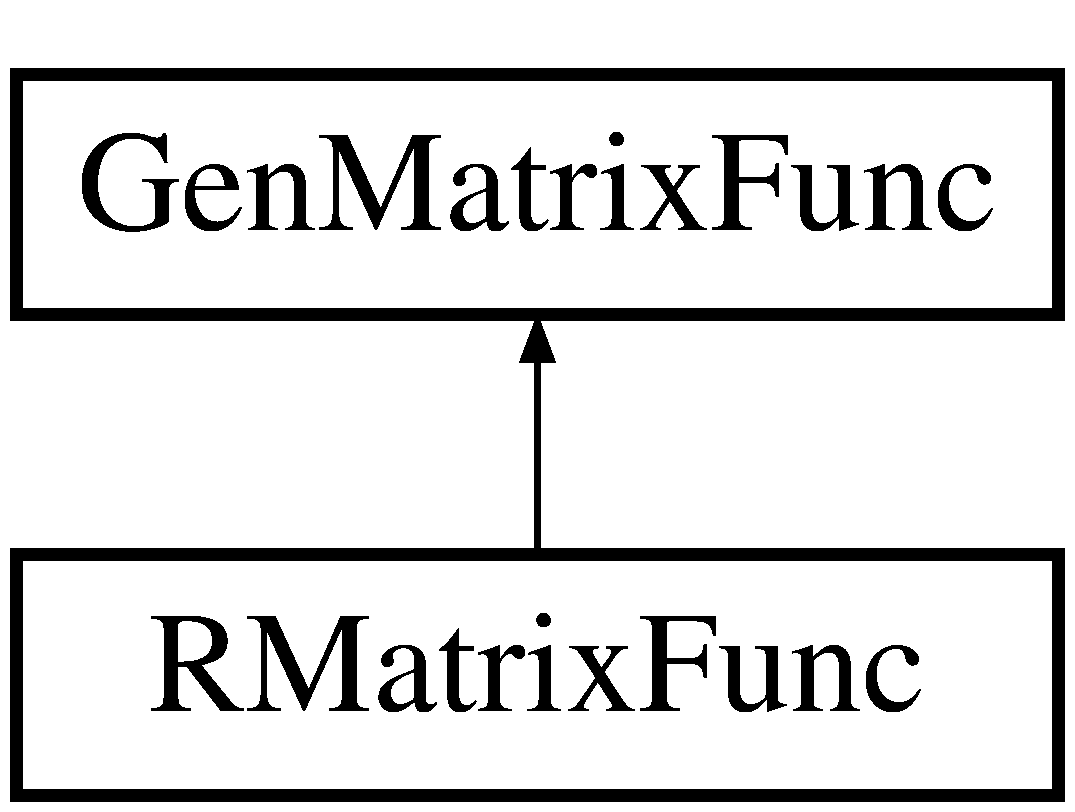
\includegraphics[height=2cm]{classRMatrixFunc}
\end{center}
\end{figure}
\subsection*{Public Member Functions}
\begin{CompactItemize}
\item 
\bf{RMatrix\-Func} (\bf{CNuc} $\ast$)
\item 
\bf{CNuc} $\ast$ \bf{compound} () const 
\item 
void \bf{Clear\-Matrices} ()
\item 
void \bf{Fill\-Matrices} (\bf{EPoint} $\ast$)
\item 
void \bf{Invert\-Matrices} ()
\item 
void \bf{Calculate\-TMatrix} (\bf{EPoint} $\ast$)
\item 
void \bf{Calculate\-Cross\-Section} ()
\item 
double \bf{Get\-RMatrix\-Element} (int, int, int) const 
\item 
std::complex$<$ double $>$ \bf{Get\-RLMatrix\-Element} (int, int, int) const 
\item 
std::complex$<$ double $>$ \bf{Get\-RLInv\-Matrix\-Element} (int, int, int) const 
\item 
std::complex$<$ double $>$ \bf{Get\-RLInv\-RMatrix\-Element} (int, int, int) const 
\item 
std::vector$<$ std::vector$<$ std::complex$<$ double $>$ $>$ $>$ $\ast$ \bf{Get\-JSpec\-RLMatrix} (int)
\item 
void \bf{Add\-RMatrix\-Element} (int, int, int, double)
\item 
void \bf{Add\-RLMatrix\-Element} (int, int, int, std::complex$<$ double $>$)
\item 
void \bf{Add\-RLInv\-Matrix} (std::vector$<$ std::vector$<$ std::complex$<$ double $>$ $>$ $>$)
\item 
void \bf{Add\-RLInv\-RMatrix\-Element} (int, int, int, std::complex$<$ double $>$)
\end{CompactItemize}


\subsection{Detailed Description}
A function class to calculate the T-Matrix using the R-Matrix. 

The \doxyref{RMatrix\-Func}{p.}{classRMatrixFunc} function class calculates the T-Matrix for a given energy point using the compound nucleus object. The \doxyref{RMatrix\-Func}{p.}{classRMatrixFunc} class is a child class of \doxyref{Gen\-Matrix\-Func}{p.}{classGenMatrixFunc}, where the cross section is calculated from the T-Matrix. 



\subsection{Constructor \& Destructor Documentation}
\index{RMatrixFunc@{RMatrix\-Func}!RMatrixFunc@{RMatrixFunc}}
\index{RMatrixFunc@{RMatrixFunc}!RMatrixFunc@{RMatrix\-Func}}
\subsubsection{\setlength{\rightskip}{0pt plus 5cm}RMatrix\-Func::RMatrix\-Func (\bf{CNuc} $\ast$ {\em compound})}\label{classRMatrixFunc_a225ad7579d7cfa0c40e54da71e986db}


The \doxyref{RMatrix\-Func}{p.}{classRMatrixFunc} object is created with reference to a \doxyref{CNuc}{p.}{classCNuc} object. 

\subsection{Member Function Documentation}
\index{RMatrixFunc@{RMatrix\-Func}!AddRLInvMatrix@{AddRLInvMatrix}}
\index{AddRLInvMatrix@{AddRLInvMatrix}!RMatrixFunc@{RMatrix\-Func}}
\subsubsection{\setlength{\rightskip}{0pt plus 5cm}void RMatrix\-Func::Add\-RLInv\-Matrix (std::vector$<$ std::vector$<$ std::complex$<$ double $>$ $>$ $>$ {\em matrix})}\label{classRMatrixFunc_2cdb7f84e8356bf35f014e96cd8af828}


This function adds an entire $ [1-RL]^{-1} $ matrix to a vector. \index{RMatrixFunc@{RMatrix\-Func}!AddRLInvRMatrixElement@{AddRLInvRMatrixElement}}
\index{AddRLInvRMatrixElement@{AddRLInvRMatrixElement}!RMatrixFunc@{RMatrix\-Func}}
\subsubsection{\setlength{\rightskip}{0pt plus 5cm}void RMatrix\-Func::Add\-RLInv\-RMatrix\-Element (int {\em j\-Group\-Num}, int {\em channel\-Num}, int {\em channel\-Prime\-Num}, std::complex$<$ double $>$ {\em matrix\-Element})}\label{classRMatrixFunc_c16e6b9095f30a66e5d16cdc94debb0d}


This function adds a $ [1-RL]^{-1}R $ matrix element specified by positions in the \doxyref{JGroup}{p.}{classJGroup} and \doxyref{AChannel}{p.}{classAChannel} vectors. \index{RMatrixFunc@{RMatrix\-Func}!AddRLMatrixElement@{AddRLMatrixElement}}
\index{AddRLMatrixElement@{AddRLMatrixElement}!RMatrixFunc@{RMatrix\-Func}}
\subsubsection{\setlength{\rightskip}{0pt plus 5cm}void RMatrix\-Func::Add\-RLMatrix\-Element (int {\em j\-Group\-Num}, int {\em channel\-Num}, int {\em channel\-Prime\-Num}, std::complex$<$ double $>$ {\em matrix\-Element})}\label{classRMatrixFunc_c9d2e6c32e32cd0b91b04767350ef7e0}


This function adds a $ [1-RL] $ matrix element specified by positions in the \doxyref{JGroup}{p.}{classJGroup} and \doxyref{AChannel}{p.}{classAChannel} vectors. \index{RMatrixFunc@{RMatrix\-Func}!AddRMatrixElement@{AddRMatrixElement}}
\index{AddRMatrixElement@{AddRMatrixElement}!RMatrixFunc@{RMatrix\-Func}}
\subsubsection{\setlength{\rightskip}{0pt plus 5cm}void RMatrix\-Func::Add\-RMatrix\-Element (int {\em j\-Group\-Num}, int {\em channel\-Num}, int {\em channel\-Prime\-Num}, double {\em matrix\-Element})}\label{classRMatrixFunc_28a73ef30a53ea24ebef4c00179d3ac5}


This function adds an R-Matrix element specified by positions in the \doxyref{JGroup}{p.}{classJGroup} and \doxyref{AChannel}{p.}{classAChannel} vectors. \index{RMatrixFunc@{RMatrix\-Func}!CalculateCrossSection@{CalculateCrossSection}}
\index{CalculateCrossSection@{CalculateCrossSection}!RMatrixFunc@{RMatrix\-Func}}
\subsubsection{\setlength{\rightskip}{0pt plus 5cm}void RMatrix\-Func::Calculate\-Cross\-Section ()}\label{classRMatrixFunc_790ee4a3d57ac489848666e676ac8f83}


Instantiated in the parent class. \index{RMatrixFunc@{RMatrix\-Func}!CalculateTMatrix@{CalculateTMatrix}}
\index{CalculateTMatrix@{CalculateTMatrix}!RMatrixFunc@{RMatrix\-Func}}
\subsubsection{\setlength{\rightskip}{0pt plus 5cm}void RMatrix\-Func::Calculate\-TMatrix (\bf{EPoint} $\ast$ {\em point})\hspace{0.3cm}{\tt  [virtual]}}\label{classRMatrixFunc_62be4a71a76ecdbb75277b62cf30f0e8}


This function calculates the T-Matrix for each reaction pathways based on the $ [1-RL]^{-1}R $ matrix. 

Implements \bf{Gen\-Matrix\-Func} \doxyref{p.}{classGenMatrixFunc_f89bf73a0a2f230c2187947520c1f360}.\index{RMatrixFunc@{RMatrix\-Func}!ClearMatrices@{ClearMatrices}}
\index{ClearMatrices@{ClearMatrices}!RMatrixFunc@{RMatrix\-Func}}
\subsubsection{\setlength{\rightskip}{0pt plus 5cm}void RMatrix\-Func::Clear\-Matrices ()\hspace{0.3cm}{\tt  [virtual]}}\label{classRMatrixFunc_ef604251f6135d99ccf051e623d76ad7}


Clears all matrices associated with the \doxyref{RMatrix\-Func}{p.}{classRMatrixFunc} object. 

Implements \bf{Gen\-Matrix\-Func} \doxyref{p.}{classGenMatrixFunc_41a9098087eac97b9c7de7aee82fa3d8}.\index{RMatrixFunc@{RMatrix\-Func}!compound@{compound}}
\index{compound@{compound}!RMatrixFunc@{RMatrix\-Func}}
\subsubsection{\setlength{\rightskip}{0pt plus 5cm}\bf{CNuc}$\ast$ RMatrix\-Func::compound () const\hspace{0.3cm}{\tt  [inline, virtual]}}\label{classRMatrixFunc_9cfee7ffe97466ba19e1e5014567713a}


Returns a pointer to the compound nucleus object. 

Implements \bf{Gen\-Matrix\-Func} \doxyref{p.}{classGenMatrixFunc_12603673326e93fb80d8db05fad085de}.\index{RMatrixFunc@{RMatrix\-Func}!FillMatrices@{FillMatrices}}
\index{FillMatrices@{FillMatrices}!RMatrixFunc@{RMatrix\-Func}}
\subsubsection{\setlength{\rightskip}{0pt plus 5cm}void RMatrix\-Func::Fill\-Matrices (\bf{EPoint} $\ast$ {\em point})\hspace{0.3cm}{\tt  [virtual]}}\label{classRMatrixFunc_7ad8de01bb08e66e2576bbb0271ff65b}


This function creates the $ [1-RL] $ and $ R $ Matrices from the \doxyref{CNuc}{p.}{classCNuc} object. 

Implements \bf{Gen\-Matrix\-Func} \doxyref{p.}{classGenMatrixFunc_0ce6fcce1afbd13bfdb753fcdfbe196c}.\index{RMatrixFunc@{RMatrix\-Func}!GetJSpecRLMatrix@{GetJSpecRLMatrix}}
\index{GetJSpecRLMatrix@{GetJSpecRLMatrix}!RMatrixFunc@{RMatrix\-Func}}
\subsubsection{\setlength{\rightskip}{0pt plus 5cm}std::vector$<$ std::vector$<$ std::complex$<$ double $>$ $>$ $>$ $\ast$ RMatrix\-Func::Get\-JSpec\-RLMatrix (int {\em j\-Group\-Num})}\label{classRMatrixFunc_26114cdd2ec140c0bbfeb7356ba0796f}


Returns an entire $ [1-RL] $ Matrix specified by a position in the \doxyref{JGroup}{p.}{classJGroup} vector. \index{RMatrixFunc@{RMatrix\-Func}!GetRLInvMatrixElement@{GetRLInvMatrixElement}}
\index{GetRLInvMatrixElement@{GetRLInvMatrixElement}!RMatrixFunc@{RMatrix\-Func}}
\subsubsection{\setlength{\rightskip}{0pt plus 5cm}std::complex$<$ double $>$ RMatrix\-Func::Get\-RLInv\-Matrix\-Element (int {\em j\-Group\-Num}, int {\em channel\-Num}, int {\em channel\-Prime\-Num}) const}\label{classRMatrixFunc_17190e37f593a1954ca8405ba67ba3e6}


Returns a $ [1-RL]^{-1} $ Matrix element specified by positions in the \doxyref{JGroup}{p.}{classJGroup} and \doxyref{AChannel}{p.}{classAChannel} vectors. \index{RMatrixFunc@{RMatrix\-Func}!GetRLInvRMatrixElement@{GetRLInvRMatrixElement}}
\index{GetRLInvRMatrixElement@{GetRLInvRMatrixElement}!RMatrixFunc@{RMatrix\-Func}}
\subsubsection{\setlength{\rightskip}{0pt plus 5cm}std::complex$<$ double $>$ RMatrix\-Func::Get\-RLInv\-RMatrix\-Element (int {\em j\-Group\-Num}, int {\em channel\-Num}, int {\em channel\-Prime\-Num}) const}\label{classRMatrixFunc_79ec1505027cddfa737cf3f04287da7a}


Returns a $ [1-RL]^{-1}R $ Matrix element specified by positions in the \doxyref{JGroup}{p.}{classJGroup} and \doxyref{AChannel}{p.}{classAChannel} vectors. \index{RMatrixFunc@{RMatrix\-Func}!GetRLMatrixElement@{GetRLMatrixElement}}
\index{GetRLMatrixElement@{GetRLMatrixElement}!RMatrixFunc@{RMatrix\-Func}}
\subsubsection{\setlength{\rightskip}{0pt plus 5cm}std::complex$<$ double $>$ RMatrix\-Func::Get\-RLMatrix\-Element (int {\em j\-Group\-Num}, int {\em channel\-Num}, int {\em channel\-Prime\-Num}) const}\label{classRMatrixFunc_8c5d6b896008bdfeb976370e7e139959}


Returns an $ [1-RL] $ Matrix element specified by positions in the \doxyref{JGroup}{p.}{classJGroup} and \doxyref{AChannel}{p.}{classAChannel} vectors. \index{RMatrixFunc@{RMatrix\-Func}!GetRMatrixElement@{GetRMatrixElement}}
\index{GetRMatrixElement@{GetRMatrixElement}!RMatrixFunc@{RMatrix\-Func}}
\subsubsection{\setlength{\rightskip}{0pt plus 5cm}double RMatrix\-Func::Get\-RMatrix\-Element (int {\em j\-Group\-Num}, int {\em channel\-Num}, int {\em channel\-Prime\-Num}) const}\label{classRMatrixFunc_9f0b4b468efed5e2c3a571ea789cb62f}


Returns an R-Matrix element specified by positions in the \doxyref{JGroup}{p.}{classJGroup} and \doxyref{AChannel}{p.}{classAChannel} vectors. \index{RMatrixFunc@{RMatrix\-Func}!InvertMatrices@{InvertMatrices}}
\index{InvertMatrices@{InvertMatrices}!RMatrixFunc@{RMatrix\-Func}}
\subsubsection{\setlength{\rightskip}{0pt plus 5cm}void RMatrix\-Func::Invert\-Matrices ()\hspace{0.3cm}{\tt  [virtual]}}\label{classRMatrixFunc_b67c0ad184bf6e38343b5c24e64a9b43}


This function inverts the $ [1-RL] $ matrices and creates the $ [1-RL]^{-1}R $ matrices. 

Implements \bf{Gen\-Matrix\-Func} \doxyref{p.}{classGenMatrixFunc_2dbfafa4c608ad5c1b27db7684f8f839}.

The documentation for this class was generated from the following files:\begin{CompactItemize}
\item 
azure\_\-v2/include/RMatrix\-Func.h\item 
azure\_\-v2/src/RMatrix\-Func.cpp\end{CompactItemize}

\section{Shft\-Func Class Reference}
\label{classShftFunc}\index{ShftFunc@{ShftFunc}}
A function class for negative energy shift functions.  


{\tt \#include $<$Shft\-Func.h$>$}

\subsection*{Public Member Functions}
\begin{CompactItemize}
\item 
\bf{Shft\-Func} (\bf{PPair} $\ast$p\-Pair)
\item 
int \bf{z1} () const 
\item 
int \bf{z2} () const 
\item 
double \bf{redmass} () const 
\item 
double \bf{total\-Sep\-E} () const 
\item 
double \bf{radius} () const 
\item 
double \bf{operator()} (int l, double energy) const 
\item 
double \bf{Energy\-Derivative} (int l, double energy) const 
\end{CompactItemize}


\subsection{Detailed Description}
A function class for negative energy shift functions. 

A shift function for negative energy channels is calculated as $ S=\rho \frac{W_c'(k\rho)}{W_c(k\rho)} $, where the prime indicates the derivative with respect to $ \rho $. The AZURE function class \doxyref{Shft\-Func}{p.}{classShftFunc} uses the GSL package to calculates the numerical derivative. 



\subsection{Constructor \& Destructor Documentation}
\index{ShftFunc@{Shft\-Func}!ShftFunc@{ShftFunc}}
\index{ShftFunc@{ShftFunc}!ShftFunc@{Shft\-Func}}
\subsubsection{\setlength{\rightskip}{0pt plus 5cm}Shft\-Func::Shft\-Func (\bf{PPair} $\ast$ {\em p\-Pair})\hspace{0.3cm}{\tt  [inline]}}\label{classShftFunc_be6d3191736d78712c237ccb6dbb602a}


The \doxyref{Shft\-Func}{p.}{classShftFunc} object is created with reference to a particle pair. 

\subsection{Member Function Documentation}
\index{ShftFunc@{Shft\-Func}!EnergyDerivative@{EnergyDerivative}}
\index{EnergyDerivative@{EnergyDerivative}!ShftFunc@{Shft\-Func}}
\subsubsection{\setlength{\rightskip}{0pt plus 5cm}double Shft\-Func::Energy\-Derivative (int {\em l}, double {\em energy}) const\hspace{0.3cm}{\tt  [inline]}}\label{classShftFunc_3c00feeb37d2279df0b98d0cb17181dd}


Returns the energy derivative of the shift function at the specified orbital angular momentum and energy in the compound system. \index{ShftFunc@{Shft\-Func}!operator()@{operator()}}
\index{operator()@{operator()}!ShftFunc@{Shft\-Func}}
\subsubsection{\setlength{\rightskip}{0pt plus 5cm}double Shft\-Func::operator() (int {\em l}, double {\em energy}) const\hspace{0.3cm}{\tt  [inline]}}\label{classShftFunc_b94abdf2446a774869cc90ab58582637}


The parenthesis operator is defined to make the class instance callable as a function. The orbital angular momentum and energy in the compound system are the dependent variables. The function returns the value of the shift function. \index{ShftFunc@{Shft\-Func}!radius@{radius}}
\index{radius@{radius}!ShftFunc@{Shft\-Func}}
\subsubsection{\setlength{\rightskip}{0pt plus 5cm}double Shft\-Func::radius () const\hspace{0.3cm}{\tt  [inline]}}\label{classShftFunc_c1506d395c2b1399866041bc5c64464f}


Returns the channel radius of the particle pair. \index{ShftFunc@{Shft\-Func}!redmass@{redmass}}
\index{redmass@{redmass}!ShftFunc@{Shft\-Func}}
\subsubsection{\setlength{\rightskip}{0pt plus 5cm}double Shft\-Func::redmass () const\hspace{0.3cm}{\tt  [inline]}}\label{classShftFunc_b44fcd8f6c029814fac975975b6c5a6f}


Returns the reduced mass of the particle pair. \index{ShftFunc@{Shft\-Func}!totalSepE@{totalSepE}}
\index{totalSepE@{totalSepE}!ShftFunc@{Shft\-Func}}
\subsubsection{\setlength{\rightskip}{0pt plus 5cm}double Shft\-Func::total\-Sep\-E () const\hspace{0.3cm}{\tt  [inline]}}\label{classShftFunc_45e84f1eddb2e2103bf5d97308e35b7b}


Returns the total seperation energy of the particle pair. \index{ShftFunc@{Shft\-Func}!z1@{z1}}
\index{z1@{z1}!ShftFunc@{Shft\-Func}}
\subsubsection{\setlength{\rightskip}{0pt plus 5cm}int Shft\-Func::z1 () const\hspace{0.3cm}{\tt  [inline]}}\label{classShftFunc_8979cf969e7d64e5eb6924a9389c4b80}


Returns the atomic number of the first particle in the pair. \index{ShftFunc@{Shft\-Func}!z2@{z2}}
\index{z2@{z2}!ShftFunc@{Shft\-Func}}
\subsubsection{\setlength{\rightskip}{0pt plus 5cm}int Shft\-Func::z2 () const\hspace{0.3cm}{\tt  [inline]}}\label{classShftFunc_fefc96a9e4be04d337c5787433fa6322}


Returns the atomic number of the second particle in the pair. 

The documentation for this class was generated from the following file:\begin{CompactItemize}
\item 
azure\_\-v2/include/Shft\-Func.h\end{CompactItemize}

\section{Temp\-TMatrix Struct Reference}
\label{structTempTMatrix}\index{TempTMatrix@{TempTMatrix}}
A temporaray T-Matrix structure.  


{\tt \#include $<$Gen\-Matrix\-Func.h$>$}

\subsection*{Public Attributes}
\begin{CompactItemize}
\item 
double \bf{j\-Value}\label{structTempTMatrix_2eacb89dce0a9f855d5e8739a3c1ec79}

\begin{CompactList}\small\item\em Total spin value of temporary matrix element. \item\end{CompactList}\item 
int \bf{l\-Value}\label{structTempTMatrix_08916dc25ae0301db669635ba6394c66}

\begin{CompactList}\small\item\em Entrance orbital angular momentum for temporary matrix element. \item\end{CompactList}\item 
int \bf{lp\-Value}\label{structTempTMatrix_10c29b33028855d3321f3c15f626b3d0}

\begin{CompactList}\small\item\em Exit orbital angular momentum for temporary matrix element. \item\end{CompactList}\item 
std::complex$<$ double $>$ \bf{TMatrix}\label{structTempTMatrix_396bc554d60212d7bd6f88c27a45a9a5}

\begin{CompactList}\small\item\em Value of temporary matrix element. \item\end{CompactList}\end{CompactItemize}


\subsection{Detailed Description}
A temporaray T-Matrix structure. 

The \doxyref{Temp\-TMatrix}{p.}{structTempTMatrix} structure is used to coherently add T-matrix elements from pathways with like $ J,l,l' $ values for the calculation of angle integrated cross section. This is primarly used to facilitate the interference between internal and external pathways. 



The documentation for this struct was generated from the following file:\begin{CompactItemize}
\item 
azure\_\-v2/include/Gen\-Matrix\-Func.h\end{CompactItemize}

\section{Whit\-Func Class Reference}
\label{classWhitFunc}\index{WhitFunc@{WhitFunc}}
A function class to calculate Whittaker functions for negative energy channels.  


{\tt \#include $<$Whit\-Func.h$>$}

\subsection*{Public Member Functions}
\begin{CompactItemize}
\item 
\bf{Whit\-Func} (\bf{PPair} $\ast$p\-Pair)
\item 
int \bf{z1} () const 
\item 
int \bf{z2} () const 
\item 
double \bf{redmass} () const 
\item 
double \bf{operator()} (int l, double radius, double energy) const 
\end{CompactItemize}


\subsection{Detailed Description}
A function class to calculate Whittaker functions for negative energy channels. 

The function class \doxyref{Whit\-Func}{p.}{classWhitFunc} uses the GSL package to calculate Whittaker functions for negative energy channels in integral form. 



\subsection{Constructor \& Destructor Documentation}
\index{WhitFunc@{Whit\-Func}!WhitFunc@{WhitFunc}}
\index{WhitFunc@{WhitFunc}!WhitFunc@{Whit\-Func}}
\subsubsection{\setlength{\rightskip}{0pt plus 5cm}Whit\-Func::Whit\-Func (\bf{PPair} $\ast$ {\em p\-Pair})\hspace{0.3cm}{\tt  [inline]}}\label{classWhitFunc_fcf3c874fd2a8704decb56b6915a2a03}


The \doxyref{Whit\-Func}{p.}{classWhitFunc} object is created with reference to a \doxyref{PPair}{p.}{classPPair} object. 

\subsection{Member Function Documentation}
\index{WhitFunc@{Whit\-Func}!operator()@{operator()}}
\index{operator()@{operator()}!WhitFunc@{Whit\-Func}}
\subsubsection{\setlength{\rightskip}{0pt plus 5cm}double Whit\-Func::operator() (int {\em l}, double {\em radius}, double {\em energy}) const\hspace{0.3cm}{\tt  [inline]}}\label{classWhitFunc_2c88474fc6d1949604e91d361be6ced8}


The parenthesis operator is defined to make the class instance callable as a function. The orbital angular momentum, binding energy, and radius are the dependent variables. The function returns the value of the Whittaker function. \index{WhitFunc@{Whit\-Func}!redmass@{redmass}}
\index{redmass@{redmass}!WhitFunc@{Whit\-Func}}
\subsubsection{\setlength{\rightskip}{0pt plus 5cm}double Whit\-Func::redmass () const\hspace{0.3cm}{\tt  [inline]}}\label{classWhitFunc_d0319a55d34110175b2282c3dfba7c6c}


Returns the reduced mass of the particle pair. \index{WhitFunc@{Whit\-Func}!z1@{z1}}
\index{z1@{z1}!WhitFunc@{Whit\-Func}}
\subsubsection{\setlength{\rightskip}{0pt plus 5cm}int Whit\-Func::z1 () const\hspace{0.3cm}{\tt  [inline]}}\label{classWhitFunc_f480d7794cee3d2e0a364a85e011a6e4}


Returns the atomic number of the first particle in the pair. \index{WhitFunc@{Whit\-Func}!z2@{z2}}
\index{z2@{z2}!WhitFunc@{Whit\-Func}}
\subsubsection{\setlength{\rightskip}{0pt plus 5cm}int Whit\-Func::z2 () const\hspace{0.3cm}{\tt  [inline]}}\label{classWhitFunc_ec97e8e760c1f07a52f7d90265d1cc7f}


Returns the atomic number of the second particle in the pair. 

The documentation for this class was generated from the following file:\begin{CompactItemize}
\item 
azure\_\-v2/include/Whit\-Func.h\end{CompactItemize}

\printindex
\end{document}
